\documentclass[12pt]{article}
\usepackage[english]{babel}
\usepackage{color,soul}
\usepackage{apacite} 
\bibliographystyle{apacite}
\usepackage{url}
\usepackage[titletoc]{appendix}
\usepackage[utf8x]{inputenc}
\usepackage{lmodern}
\usepackage{listings}
\usepackage{amsmath}
\usepackage{courier}
\usepackage{wrapfig}
\usepackage[export]{adjustbox}
\usepackage[bottom]{footmisc}
\usepackage{graphicx}
\usepackage{hyperref}
\usepackage{tcolorbox}
\usepackage{pdfpages}
\usepackage{graphicx}
\usepackage[section]{placeins}
\usepackage{enumitem}
\usepackage{comment}
\graphicspath{{images/}}
\usepackage{parskip}
\usepackage{flafter}
\usepackage{colortbl}
\usepackage{fancyhdr}
\usepackage{csvsimple}
\usepackage{booktabs}
\usepackage{longtable}
\usepackage{multirow}
\usepackage{vmargin}
\usepackage{listings}
\usepackage{pgfplotstable,filecontents}
\usepackage{natbib}
\usepackage{subfigure}
\usepackage{graphicx}
\usepackage{sidecap}
\usepackage{floatrow}
\usepackage{framed}
\usepackage[T1]{fontenc}
\usepackage{babel}
\usepackage{listings}
\usepackage[font=small,labelfont=bf]{caption}
\newfloatcommand{capbtabbox}{table}[][\FBwidth]
\usepackage{blindtext}
\usepackage[section]{placeins}
\usepackage{csvsimple}
\setlength{\bibsep}{5.0pt}
\pgfplotsset{compat=1.9}% supress warning
\setmarginsrb{2.0cm}{1.0cm}{2.0cm}{1.0cm}{1.0cm}{1.0cm}{1.0cm}{1.0cm}
\usepackage{color}
\usepackage{minted}
\usepackage{array}
\usepackage{longtable}

\newcolumntype{L}[1]{>{\raggedright\let\newline\\\arraybackslash\hspace{0pt}}m{#1}}
\newcolumntype{C}[1]{>{\centering\let\newline\\\arraybackslash\hspace{0pt}}m{#1}}
\newcolumntype{R}[1]{>{\raggedleft\let\newline\\\arraybackslash\hspace{0pt}}m{#1}}
\definecolor{dkgreen}{rgb}{0,0.6,0}
\definecolor{gray}{rgb}{0.5,0.5,0.5}
\definecolor{mauve}{rgb}{0.58,0,0.82}
\definecolor{black}{rgb}{0,0,0}
\definecolor{white}{rgb}{1,1,1}
\definecolor{blue}{rgb}{0,0,1}
\definecolor{red}{rgb}{1,0,0}
\lstset{ 
  language=C++,                         
  basicstyle=\scriptsize,       
  numbers=left,                   		% where to put the line-numbers
  numberstyle=\tiny\color{gray},  	% the style that is used for the line-numbers
  stepnumber=1,                   		% the step between two line-numbers. If it's 1, each line will be numbered
  numbersep=5pt,                  		% how far the line-numbers are from the code
  backgroundcolor=\color{white},  	% choose the background color. must add \usepackage{color}
  showspaces=false,               		% show spaces adding particular underscores
  showstringspaces=false,        		 % underline spaces within strings
  showtabs=false,                		 % show tabs within strings adding particular underscores
  frame=single,                  			 % adds a frame around the code
  rulecolor=\color{black},       		 % if not set, the frame-color may be changed on line-breaks within not-black text (e.g. commens (green here))
  tabsize=2,                      			% sets default tabsize to 2 spaces
  captionpos=b,                   		% sets the caption-position to bottom
  breaklines=true,               		 % sets automatic line breaking
  breakatwhitespace=false,       		 % sets if automatic breaks should only happen at whitespace
  title=\lstname,                 			% show the filename of files included with \lstinputlisting;
                                 				 % also try caption instead of title
  keywordstyle=\color{blue},      		% keyword style
  commentstyle=\color{dkgreen},  	 % comment style
  stringstyle=\color{mauve},      		% string literal style
  escapeinside={\%*}{*)},         		% if you want to add a comment within your code
  morekeywords={*,...}           		 % if you want to add more keywords to the set
} 

\newtheorem{esti}{Theorem}[section]
\title{CS3201/2 Iteration 3}					% Title
% * <akankshita.dash@u.nus.edu> 2017-09-06T05:26:27.242Z:
%
% ^.	

\makeatletter
\let\thetitle\@title
\let\theauthor\@author
\let\thedate\@date
\makeatother
\author{}
\pagestyle{fancy}
\fancyhf{}
\rhead{\theauthor}
\lhead{\thetitle}
\cfoot{\thepage}
\usepackage{setspace}
\begin{document}
\doublespacing
%%%%%%%%%%%%%%%%%%%%%%%%%%%%%%%%%%%%%%%%%%%%%%%%%%%%%%%%%%%%%%%%%%%%%%%%%%%%%%%%%%%%%%%%%

%%%%%%%%%%%%%%%%%%%%%%%%%%%%%%%%%%%%%%%%%%%%%%%%%%%%%%%%%%%%%%%%%%%%%%%%%%%%%%%%%%%%%%%%%

\begin{titlepage}
	\centering
    
\includegraphics[width = 0.4\textwidth]{logo1.jpg}\\[0.4cm]	% University Logo
    \textsc{ National University of Singapore}\\[0.2 cm]	% University Name
	\rule{\linewidth}{0.2 mm} \\[0.1 cm]
	{ \huge \bfseries \thetitle}\\
    \rule{\linewidth}{0.2 mm} \\[0.2 cm]
			\begin{center} 
            \textbf{13th November 2017}\\[0.7cm]
			\textbf { SEM 1, AY2017/2018}\\[0.7cm]
			\emph{Submitted By :} \\[0.1cm]
           
      \textbf{\underline{Team 11}}    
      \subsubsection*{Consultation Hour: Tuesday, 1:00-2:00 pm}
 \begin{table}[htbp]
\begin{tabular}{|c|c|c|}
\hline
\textbf{Team Member} & \textbf{E-mail} & \textbf{Phone number}\\\hline
Akankshita Dash & akankshita.dash@u.nus.edu & 84010419  \\
\hline
Chua Ping Chan & a0126623@u.nus.edu & 90876406 \\
\hline
Lau Wen Hao & a0121528@u.nus.edu & 84991295  \\
\hline
Marcus Ng & marcusngwenjian@u.nus.edu
 & 97502493  \\
\hline
Zhang Ying & e0006954@u.nus.edu
 & 82289895  \\
\hline
Zhuang Lei & e0003940@u.nus.edu
 & 98374236 \\
\hline
\end{tabular}
\end{table}
		    \end{center}
        


\end{titlepage}

%%%%%%%%%%%%%%%%%%%%%%%%%%%%%%%%%%%%%%%%%%%%%%%%%%%%%%%%%%%%%%%%%%%%%%%%%%%%%%%%%%%%%%%%%

%%%%%%%%%%%%%%%%%%%%%%%%%%%%%%%%%%%%%%%%%%%%%%%%%%%%%%%%%%%%%%%%%%%%%%%%%%%%%%%%%%%%%%%%%
\tableofcontents
\newpage
\singlespacing
\section{Scope of SPA Implementation}
Our SPA meets all the requirements for Iteration 3 and is fully operational.
\subsection{Parser}
Our \textbf{SPA}, internally referred to as \textbf{SPAXI}, is now able to parse a SIMPLE program completely and update PKB with the correct relations.
\subsection{PKB}
PKB supports \textbf{Affects, Affects*} in addition to previous implementations of \textbf{Follows, Follows*, Parent, Parent*, Uses, Modifies, Pattern, Calls, Calls*, Next and Next*}. It also supports Statement List.
\subsection{PQL}
The QueryProcessor is able to evaluate PQL Queries with multiple \textbf{such that, pattern} and \textbf{with} clauses. In addition to \textbf{Select} \textbf{BOOLEAN} and \textbf{Select synonym}, it can also support selection of \textbf{attributes} and \textbf{Select <tuple>.}
\subsection{Special Achievements}
Our testing team automated System Testing, making debugging a lot faster and easier. Further details are given in the testing section.
\section{Development Plan}
\subsection{Development Plan for SPA}
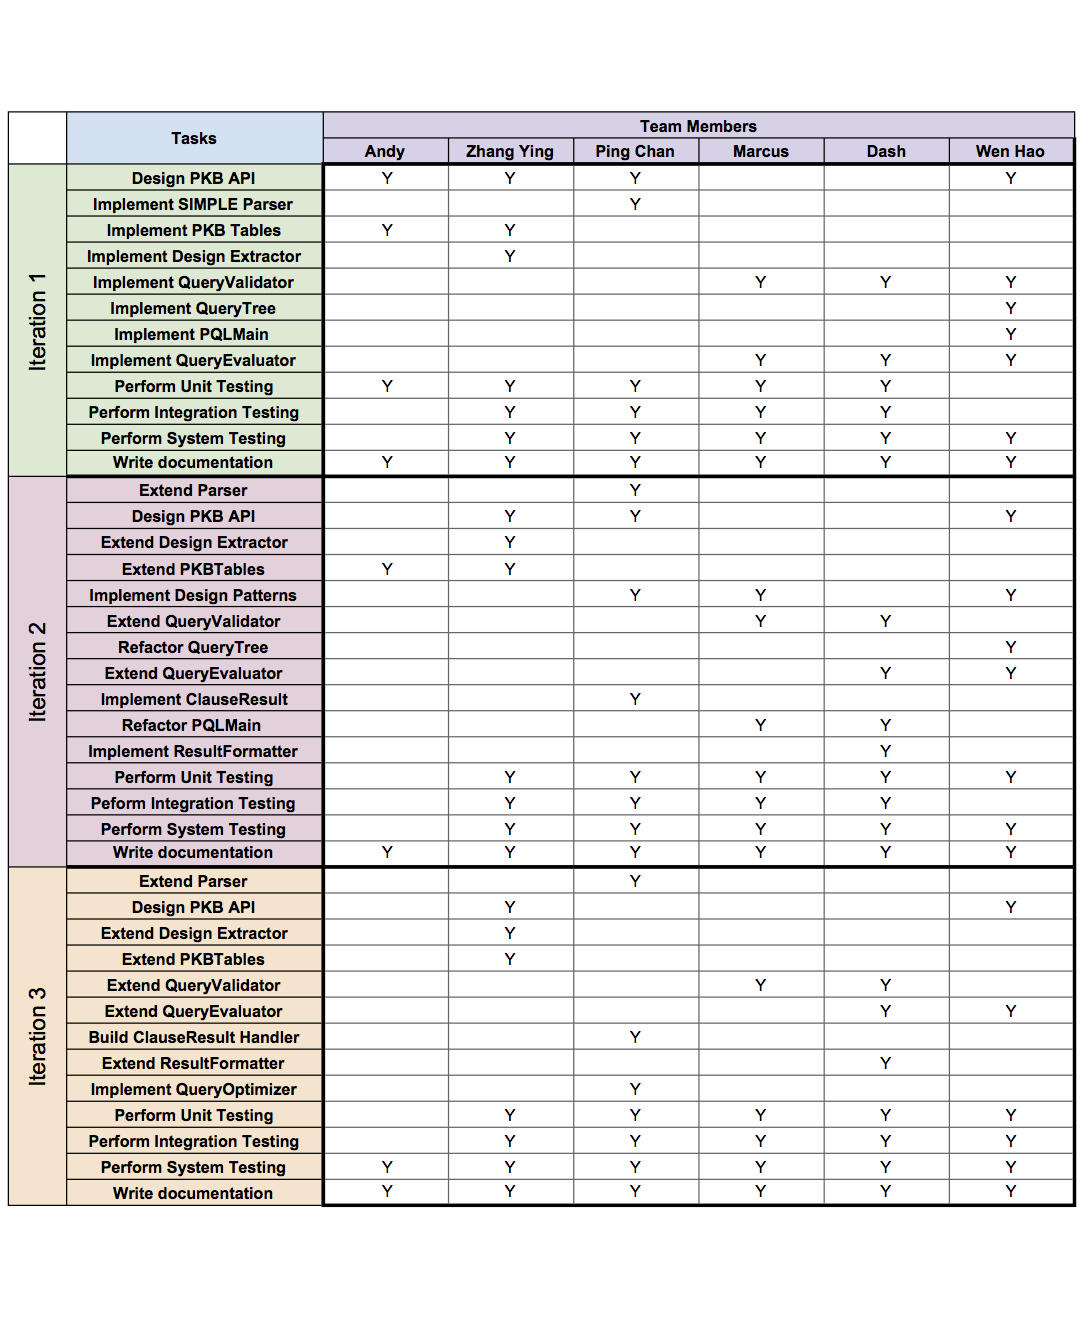
\includegraphics[width = 1.2\textwidth,center]{WholePlan.jpg}
\subsection{Development Plan for Iteration 3}
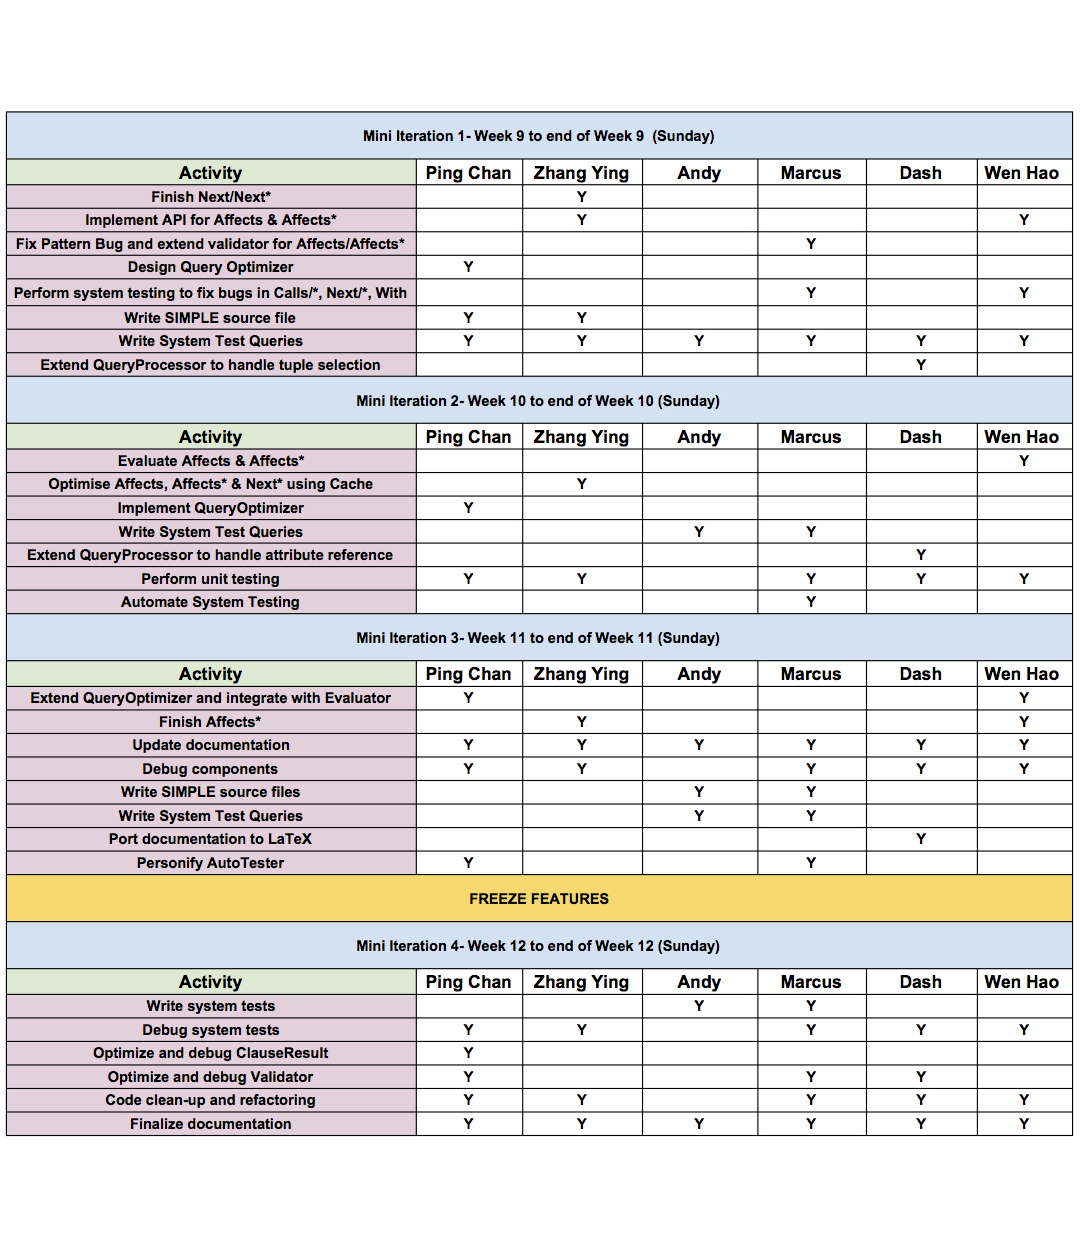
\includegraphics[width = 1.1\textwidth,center]{Iteration3.jpg}
\newpage
\section{SPA Design}
\subsection{Overview}
\begin{figure}[!htb].
\centering
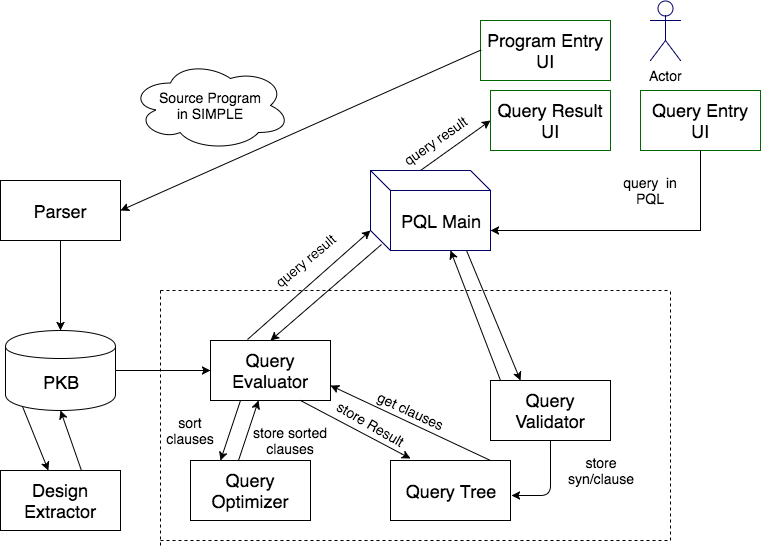
\includegraphics[width=1.0\textwidth]{Architecture_Diagram.png}
\caption{\label{fig:Architecture}Main components of SPA}
\end{figure}
In  SPA, there are two main components:
\begin{enumerate}
\item Program Knowledge Base (PKB)
\item Program Query Language (PQL)
\end{enumerate}

Our SPA design is very similar to the original proposed design. In addition to the proposed components, we implemented PQL Main and Query Optimiser. PQL Main controls the flow of all the other components in PQL and decides the sequence during query processing, while Query Optimiser decides the order of evaluation in a query with multiple clauses.

\subsection{Design of SPA Components}

\subsubsection{Parser }
In SPA, Parser is responsible for parsing a given SIMPLE source code, validating the syntax, extracting information and storing it in PKB.

Whenever the Parser detects a syntax error, it will stop parsing the SIMPLE source and display an error feedback message to the user. The Parser will finish parsing and allow queries to be evaluated only if the SIMPLE source code is syntactically correct.

At the beginning of the parsing process, the Parser reads a given SIMPLE source file into a concatenated string, which is stored in-memory in a class attribute.

After the SIMPLE source content is extracted into a concatenated string, the Parser will make one parse, just to ensure all the braces pairs up correctly. If there is a mismatch in the way the braces pair-up, the Parser will output a feedback message to indicate the syntax error and stop parsing at once.

If all the braces are paired up well, the Parser is ready to Parse the SIMPLE source contents line by line. The Parser implemented is a predictive recursive descent parser, whereby the concatenated SOURCE string will be tokenized; the Parser starts by reading a token, and then determines what is the next token to expect.
\begin{center}
\fbox{\begin{minipage}{35em}
\begin{center}\textbf{Parser’s Tokenizer}
\end{center}
The tokenizer of the parser is made such that if given a SIMPLE program: \newline \vspace{0.5mm}
\texttt{\noindent procedure First \{
   \newline 1 \hspace{3mm}	abc123 = 100 * x3;
   \vspace{0.5mm}
\newline\hspace{1mm}\} \vspace{0.5mm}}
\newline The tokenizer will break the string down to a list of tokens containing:
‘procedure’, ‘First’, ‘\{’, ‘abc123’, ‘=’, ‘$100$’, ‘*’, ‘$x3$’, ‘;’ and ‘\}’.
Any interleaving whitespace will be ignored.
\end{minipage}}
\end{center}
\vspace{6mm}For example, 
at the very beginning of the SIMPLE source,
the Parser invokes a member function that parses procedure,
and expects the upcoming token to be the keyword “procedure”. 
If the first token indeed matches the keyword, 
the Parser will move on to the next token and validate whether
it is a valid procedure name or not, according to the SIMPLE grammar rules. If it is valid,
the Parser will add the name 
of procedure into PKB. It will then expect an open brace character ‘\{‘ next, and so on.

Similar to parsing procedure, the Parser contains various methods to parse different entities such as statement lists, assignment statements, call statements, while statements and if-else statements. Each of these methods will ensure the SIMPLE source satisfies the grammar rules, e.g. correct operands, correct expressions in assignment statements, etc. If any syntax error is detected, Parser will throw an exception and stop parsing.

After the Parser finishes parsing a SIMPLE source, it signals to PKB that it is finished, so that the Design Extractor within PKB starts computing transitive relations, e.g. Follows*, Parent*, Calls*, Next* and inter-procedural relations such as Uses and Modifies.

Do note that our Parser does not allow the LHS of assignment statements to have variables with names that conflict with (if/while/call) keywords. 

For example, \begin{verbatim} while = a; \end{verbatim}
is not allowed by our Parser. 
However, our Parser allows \begin{verbatim} a = while; \end{verbatim}
\textbf{Uses/Modifies Relation:} The Parser adds the Modifies and Uses relationship into PKB as and when the Parser parsers the relevant statements. No additional data structures are required to store any information for adding Uses/Modifies relations.

\textbf{Follows Relation:} The Parser maintains a stack of statements in order to add Follows relations to PKB. Each inner stacks represents the statement list within a code block in the correct order, and the outer stack is used to store the information of nested statement lists due to container statements.

As each inner stack represents a statement list with statements in the correct order, at the end of a code block, Parser can pop the top-most statement list in the stack and process it by setting the Follows relation based on the sequence of statements in the code block. \newline

Consider the following source code:
\begin{center}
\fbox{\begin{minipage}{35em}
\texttt{procedure First \{
\newline1 \hspace{3mm}	i = 1;
\newline2 \hspace{3mm}	b = 200;
\newline3 \hspace{3mm} c = a;
\newline4 \hspace{3mm} while a \{
\newline5 \hspace{12mm}		c = b - 5;
\newline6	\hspace{12mm}	b = c - a;
\newline7	\hspace{12mm}	x = x + 1; 
\newline \phantom{he} \}
\newline    8 \hspace{3mm}  d = 300;
\}}
\end{minipage}}
\end{center}
\vspace{10mm}
The stack of statements stacks will be empty at first. While beginning to parse statement 1, since it is the first statement in a new statement list, an empty stack of statement will be created and pushed onto the stack of statements stacks. Statement 1, 2, 3 and 4 will then be pushed onto the inner stack in order. When parsing statement 5, as it is a new statement in a new nested statement list, another inner stack will be created. Statements 5, 6, 7 will then be added to this new inner stack and pushed into \_stackOfFollowsStack. At the end of parsing statement 7, upon exiting the code block of the while statement, the top stack (marked in green) will be popped, and the follows relation among statements 5, 6 and 7 will be added to PKB. Then, statement 8 will be pushed to the blue statements stack. At the end of parsing statement 8, the end of procedure is reached, therefore the blue stack will be popped and the Follows relations amongst statements 1, 2, 3, 4 and 8 will be added to the PKB.
\begin{figure}[H]
  \caption{Keeping Track of Follows Relationship}
  \centering
    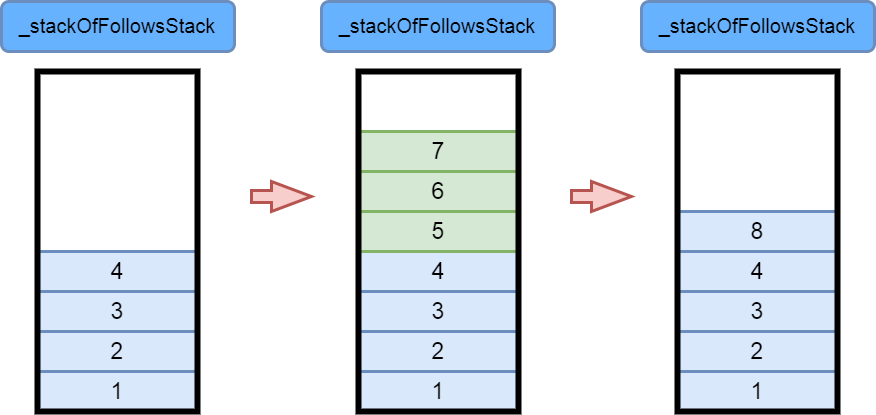
\includegraphics[width=0.7\textwidth]{Parser_AddingFollowsRelationToPKB.png}
\end{figure}

\textbf{Parent Relation:} The Parser maintains a stack called \_parentStack to keep track of the Parent relationship. Every time a parser encounters a container statement, that statement will be pushed into this stack. When exiting a container statement, the top most element of the stack will be popped. That way, while parsing the statements within a statement list of a nested container statement, the Parser will always be able to know all the Parents and transitive Parents (Parent*) while setting relations like Uses and Modifies in PKB. 
\newline
Consider the following source code:
\begin{center}
\fbox{\begin{minipage}{35em}
\texttt{procedure First \{
\newline1 \hspace{3mm}	i = 1;
\newline2 \hspace{3mm}	b = 200;
\newline3 \hspace{3mm} c = a;
\newline4 \hspace{3mm} while a \{
\newline5 \hspace{12mm}		c = b - 5;
\newline6	\hspace{12mm}	b = c - a;
\newline7	\hspace{12mm}	x = x + 1; 
\newline \phantom{he} \}
\newline    8 \hspace{3mm}  d = 300;
\}}
\end{minipage}}
\end{center}
\vspace{10mm}
When the Parser parses statement 7, the state of the \_parentStack would be as shown in the figure below:

\begin{figure}[H]
  \caption{Keeping Track of Transitive Parents}
  \centering
    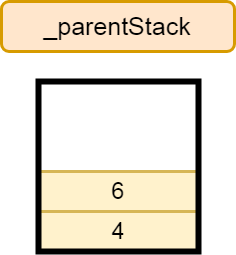
\includegraphics[width=0.2\textwidth]{Parser_AddingParentRelationToPKB.png}
\end{figure}
\textbf{Calls Relation
:} To add calls relation to PKB, the Parser will need to know the current procedure being parsed at all times. Hence, the Parser has a private attribute to store this information. When parsing a procedure call statement, the Parser validates the name of the procedure being called, and adds to PKB a call relation between the current procedure and the called procedure.\newline

\textbf{Next Relation
:} The Parser maintains a few data structures to add the Next relation to PKB: 
\begin{enumerate}
\item An unordered\_set<int> named \_prevReachableStmts that stores all the statements that can reach the current statement in one step in the control-flow graph.
\item When parsing the statements inside a while-statement, a variable called whileStmtNumber is used to store the statement number of the while-statement.
\item When parsing the statement lists inside an if-else statement, a variable called ifElseStmtNumber is used to store the statement number of the if-else statement.
\end{enumerate}
Consider the following source code. 
\begin{center}
\fbox{\begin{minipage}{35em}
\texttt{procedure ABC \{
\newline1 \hspace{3mm}	a = 1;
\newline2 \hspace{3mm}	b = 2;
\newline3 \hspace{3mm} while x \{
\newline4 \hspace{12mm}  c = 4;
\newline5 \hspace{12mm}		if x then \{
\newline6	\hspace{21mm}	i = 6;
\newline \phantom{h} \hspace{12mm}	\} else \{ 
\newline7 \hspace{21mm} j= 7;
\newline \phantom{h} \hspace{11mm} \}
\newline8 \hspace{12mm}  k = 8;
\newline \phantom{h} \hspace{3mm} \}
\newline9 \hspace{3mm} m = 9;
\newline \}}
\end{minipage}}
\end{center}
\vspace{10mm}
Whenever the Parser adds the Follows relation in PKB as described earlier, it also adds the Next relation. \newline

When parsing normal statements in the same statement list, such as going from statement 1 to statement 2, Parser will add statement 1 into \_prevReachableStmts, and use it to call setNext(\_prevReachableStmts, 2) when parsing statement 2. Before moving on to statement 3, \_prevReachableStmts is cleared and statement 2 is added into it. This process is repeated if there are more statements in the same statement list without container statements. For the case of container statements, the way Parser sets the Next relation in PKB when parsing while-statements and if-else statements will be described separately for greater clarity. \newline

\textbf{While-statement:}
In the above example, when parsing statement 3, Parser will store the statement number in the variable whileStmtNumber. Here, Parser will call PKB’s API setNext(3, 4), and then proceeds to parse all the statements in the while-block as per normal. When Parser reaches the last statement in the while-block, i.e. statement 8, it will call setNext(8, whileStmtNumber). Here, statements 8 and the whileStmtNumber will be added to the \_prevReachableStmts because these two statements have a 1-hop distance to the statement outside the while-block (if any). Upon exiting the while-block, i.e. parsing statement 9, Parser will call setNext(s, 9) for all s that are present in \_prevReachableStmts, and \_prevReachableStmts is cleared. \newline

\textbf{if-else statement:}
When parsing statement 5, Parser will store the statement number of the if-else statement in an integer variable called ifElseStmtNumber. Parser then calls setNext(ifElseStmtNumber, 6). Before exiting the if-block, the last statement number in the if-block is stored in a variable called ifBlockExitPoint. When parsing the first statement in the else-block, Parser will call setNext(ifElseStmtNumber, 7). Before exiting the else-block, \_prevReachableStmts is cleared and the last statement of the if- and else- blocks are added to \_prevReachableStmts. Upon exiting the if-else block, setNext(s, 8) is called for all s that are present in \_prevReachableStmts, and \_prevReachableStmts is cleared.

\subsubsection{PKB}
Program Knowledge Base (PKB) stores the different program design abstractions. Table-driven approach is used for the design of the PKB structure. Not only does it provides a simple yet powerful way to achieve flexibility, but it also allows quick access of the data. Different class table files were made according to the different design entities. This allows easier additions of new design entities and eases code extension as well as reducing modifications required.
\newline 

PKB contains the following components:

\begin{itemize}
\item PKB Main 
\item Procedure Index Table
\item Variable Index Table
\item Constant Table
\item Uses Table
\item Modifies Table
\item Pattern Table
\item Follows/Follows* Table
\item Parents/Parent* Table
\item Calls/Calls* Table
\item Next Table
\end{itemize}
\vspace{2mm}
\textbf{PKB-Main:} PKB-Main controls and stores all the tables in the entire PKB component. It is used by SPA front-end Parser and Query Processor components in order to reduce coupling. The APIs of the PKB-Main play a central role in the SPA architecture. \vspace{6mm}
 \newline
\textbf{\underline{Procedure Index Table:}}
\newline The Procedure Index Table stores all the procedures and their respective indexes. Before the parser starts parsing the SIMPLE source code, the procedure index is initialized to an arbitrary value of 0. Whenever a new procedure is added to its table by the Parser, an index will be generated by the Procedure Index Table and used as a key for the procedure name.

Its structure is as follows:

\underline{ProcIdxTable.h}
\begin{itemize}
\item unordered\_map<string procName, int procIndex> procIdxMap
\item unordered\_map<int procIndex, string procName> procNameMap
\item int procIdx (initialized to 0, to generate indexes for procedures)
\end{itemize}
\vspace{6mm}
\textbf{\underline{Variable Index Table
}}
\newline The Variable Index Table is stored in a similar fashion as the Procedure Index Table.

Its structure is as follows:

\underline{VarIdxTable.h}
\begin{itemize}
\item unordered\_map<string varName, int varIndex> varIdxMap
\item unordered\_map<int varIndex, string varName> varNameMap
\item int varIdx (initialized to 0, to generate indexes for indexes)
\end{itemize}
\vspace{6mm}
\textbf{\underline{Statement Type List
}}
\newline The Statement Type List stores all the statement numbers added by the Parser according to the respective entities. 

For example, if the statement number is an assignment statement, it is stored in the \textbf{assignList}. Similarly, statement number of the while statement is stored in \textbf{whileList}.  As such, when QueryEvaluator asks for assign or while statements, we are able to either retrieve the statement numbers that belong to a requested entity by filtering away unwanted data.

Its structure is as follows:

\underline{StmtTypeList.h}
\begin{itemize}
\item list<int> allStmtList, to store statement numbers with entity ‘STMT’
\item list<int> assignStmtList, to store statement numbers with entity ‘ASSIGN’
\item list<int> whileStmtList, to store statement numbers with entity ‘WHILE’
\item list<int> ifStmtList, to store statement numbers with entity ‘IF’
\item list<int> callsStmtList, to store statement numbers with entity ‘CALLS’
\end{itemize}
\vspace{6mm}
\textbf{\underline{Constant Table
}}\newline
The Constant Table stores all the constants added by the Parser. The statement number is stored in the key and the constants are stored as the value. The table will be accessed when QueryEvaluator calls ‘Select c’. 

Its structure is as follows:

\underline{ConstantTable.h}
\begin{itemize}
\item unordered\_map<int,   list<int> > constantTableMap
\end{itemize}
\vspace{6mm}
\textbf{\underline{Uses Table
}}
\newline The Uses Table stores all the Uses relationships extracted by the Parser in the form of hash maps (UsesTableStmtToVar) where the integer statement number or integer procedure index are keys, and a list of integer variable indexes are values. Firstly, when the design abstraction for Uses is added by the Parser, the raw variable (or procedure) input in the form of string is converted to a variable (or procedure) index. Both the statement number and resultant integer index are then added to the hash map. Additionally, PKB also adds the reverse relationship internally to another hash map called UsesTableVar, where integer variable (or procedure) indexes as stored as keys, and statement numbers as values. UsesTableVar contains multiple maps such that the design abstraction can be stored according to the entity of the statement, so as to facilitate retrieval when queries such as Uses(a,v) and Uses(w, v) are called by the QueryEvaluator.

\underline{UsesTableStmtToVar.h}
\begin{itemize}
\item unordered\_map<int stmtNum, list<int varIdx> > usesStmtToVarMap
\end{itemize}

\underline{UsesTableProcToVar.h}
\begin{itemize}
\item unordered\_map<int procIdx, list<int varIdx> > usesProcToVarMap
\end{itemize}

\underline{UsesTableVar.h}
\begin{itemize}
\item unordered\_map<int varIdx, list<int stmtNum> > usesVarToStmtMap
\item unordered\_map<int varIdx, list<int assignNum> > usesVarToAssignMap
\item unordered\_map<int varIdx, list<int procIdx> > usesVarToProcMap
\item unordered\_map<int varIdx, list<int whileStmtNum> > usesVarToWhileStmtMap
\item unordered\_map<int varIdx, list<int ifStmtNum> > usesVarToIfMap
\end{itemize}

\vspace{6mm}

\textbf{\underline{Modifies Table
}}
\newline The Modifies Table is populated similar to the Uses Table. \newline \newline
\underline{ModTableStmtToVar.h}
\begin{itemize}
\item unordered\_map<int stmtNum, list<int varIdx> > modStmtToVarMap
\end{itemize}
\underline{ModTableProcToVar.h}
\begin{itemize}
\item unordered\_map<int procIdx, list<int varIdx> > modProcToVarMap
\end{itemize}
\underline{ModTableVar.h}
\begin{itemize}
\item unordered\_map<int varIdx, list<int stmtNum> > modVarToStmtMap
\item unordered\_map<int varIdx, list<int assignNum> > modVarToAssignMap
\item unordered\_map<int varIdx, list<int procIdx> > modVarToProcMap
\item unordered\_map<int varIdx, list<int whileStmtNum> > modVarToWhileStmtMap
\item unordered\_map<int varIdx, list<int ifStmtNum> > modVarToIfMap
\end{itemize}
\vspace{6mm}

\textbf{\underline{Pattern Table
}}
\newline The Pattern Table stores the patterns of all assignment, while, and if statements extracted by the parser. 

The pattern is stored as follows:\newline
\textbf{Key }- statement number in the form of integer.\newline
\textbf{Value} - a pair containing LHS variable and a postfix expression of the RHS in that statement number. \newline
When the pattern is added by the parser, the LHS variable is stored as a variable index with a type integer, whereas for the RHS expression, the raw input in the form of infix expression is internally converted into postfix by the Pattern Table. The first argument of pattern-while and pattern-if clauses are defined as control variables. This table will be accessed when pattern clauses are called by the Query Evaluator. Postfix is used in this table instead of infix in order to facilitate partial matching of the subexpression. 
\newline The steps below show how the partial matching is processed in general.
\begin{enumerate}
\item Raw input in the form of infix sub-expressions are passed to the function called hasPartialMatch(stmt, expression)
\item Within the function, the infix sub-expression is converted to postfix.
\item The postfix sub-expression performs the partial match by checking with the stored expression (postfix) that is retrieved from the pattern table.
\item If both expressions match, the function returns true.
\end{enumerate}
For example, given an infix expression \textbf{“a+b*(c-d)”}, based on the rule of query evaluation, subexpression \textbf{“c-d”} partially matches using postfix, however, \textbf{“a+b”} does not, even though both expressions are the substrings of \textbf{“a+b*(c-d)”}. Hence partial matching is processed as shown:
\textbf{“a+b*(c-d)”} is converted to \textbf{list(“a”,”b”,”c”,”d”,”-”,”*”,”+”)}
The subexpressions \textbf{“c-d”} and \textbf{“a+b”} are also converted to \textbf{list(“c”,”d”,”-”)} and \textbf{list(“a”,”b”,”+”)} respectively.
\textbf{list(“c”,”d”,”-”)} is the sublist of \textbf{list(“a”,”b”,”c”,”d”,”-”,”*”,”+”)}, whereas \textbf{list(“a”,”b”,”+”)}
Hence it can be deduced that \textbf{“c-d”} is the sub-expression of \textbf{“a+b*(c-d)”}, whereas \textbf{“a+b”} is not) 

The structure of the table as follows:

{\underline{FollowsTable.h}
\begin{itemize}
\item unordered\_map<int stmtNum, pair<int LHS, list<string> RHSexpression> > assignPatternTableMap
\item unordered\_map<int stmtNum, pair<int LHS, int controlVar> > whilePatternTableMap
\item unordered\_map<int stmtNum, pair<int LHS, int controlVar> > ifPatternTableMap
\end{itemize}
\vspace{6mm}

\textbf{\underline{Follows/Follows* table}}
\newline The Follows and Follows* Tables store all the Follows and Follows* relationships respectively. When the design abstraction Follows is parsed by the Parser, it adds the statement number as a key, and the statements that the current statement follows as a value (in the form of a pair<followedBy, follows>). Follows* relationships are then computed by the Design Extractor. The table will be accessed when Follows(s1,s2) and Follows*(s1,s2) are called by the QueryEvaluator. 

The structure is as follows: 

{\underline{FollowsTable.h}
\begin{itemize}
\item unordered\_map<int stmtNum, pair<int followedBy, int follows> > followsMap
\end{itemize}
{\underline{FollowsStarBefore.h}
\begin{itemize}
\item unordered\_map<int stmtNum, list<int> followedBy> followsStarBefore;
\end{itemize}
{\underline{FollowsStarAfter.h}
\begin{itemize}
\item unordered\_map<int stmtNum, list<int> follows> followsStarAfter;
\end{itemize}
\vspace{6mm}

\textbf{\underline{Parent/Parent* table}}
\newline The Parent and Parent* Tables store all the Parent and Parent* relationships respectively. When the design abstraction Parent is added by the Parser, the statement number is added to the hash map as a key, and the list of its children of its respective statements is added as a value. A reverse version of the hash map is implemented, so as to allow computation of the parent statement of the input. Parent* relationship is then computed by the Design Extractor. The table will be accessed when Parent(s1,s2) and Parent*(s1,s2) are called by the QueryEvaluator. 

The structure is as follows: 

{\underline{ParentToChildTable.h}
\begin{itemize}
\item unordered\_map<int parent, list<int> children> parentToChildMap
\end{itemize}
{\underline{ChildToParentTable.h}
\begin{itemize}
\item unordered\_map<int child, int parent> childToParentMap
\end{itemize}
{\underline{ParentToChildStarTable.h}
\begin{itemize}
\item unordered\_map<int parent, list<int> children> parentToChildStarMap
\end{itemize}
{\underline{ChildToParentStarTable.h}
\begin{itemize}
\item unordered\_map<int child, list<int> parents> childToParentStarMap
\end{itemize}
\vspace{6mm}

\textbf{\underline{Calls/Calls* table}}
\newline The Calls and Calls* Tables store all the Calls and Calls* relationships respectively. They also store the mapping of procedures as that is needed to compute transitive closures of Uses and Modifies relationships. Calls* relationship is then computed by the Design Extractor. 

The structure is as follows: 

{\underline{CallsTable.h}
\begin{itemize}
\item unordered\_map<int, list<int> > callsProcMap
\item unordered\_map<int, list<int> > callsProcMapReverse
\end{itemize}
{\underline{CallsStarTable.h}
\begin{itemize}
\item unordered\_map<int, list<int> > callsStarProcMap
\item unordered\_map<int, list<int> > callsStarProcMapReverse
\end{itemize}
\textbf{\underline{NextTable}}
\newline The Next Table stores all the Next relations. It also acts as an adjacency list for the control flow graph which will be used for the computation of Next* relations.

The structure is as follows: 

{\underline{NextTable.h}
\begin{itemize}
\item unordered\_map<int, list<int> > nextMap
\item unordered\_map<int, list<int> > nextMapReverse
\end{itemize}
\vspace{6mm}

\textbf{\underline{Next*}}\newline
As Next* can only be computed on the fly whenever a query comes in, it will not be computed in the design extractor. It is computed in next table using the already stored information in NextTable. The computation of Next* is using a breadth-first iteration on all Next relations depending on the query type. Only the result of a Next* query with two synonym would be cached as it will contain all Next* relations for future clauses. \vspace{6mm} \newline
{\underline{\textbf{Cache}}\newline
The cache stores information regarding Next*, Affects and Affects* that was computed during the evaluation of the given query. The purpose of the cache is to avoid recomputing the aforementioned relations if there are multiple same such-that clauses. 

For example, in this query \begin{verbatim}
Select a such that Affects*(a, a1) and Affects*(1, 17)
\end{verbatim} 
PKB would compute all the Affects* relations(for Affects*(a, a1)) and store them in the cache such that the required information for the next clause(Affect*(1, 17)) is retrieved in constant time. The same could be said for Next* and Affects. The cache is cleared after the evaluation of each query.

The structure of the Cache is as follows:

\begin{itemize}
\item unordered\_map<int, list<int> > nextStarMapList/nextStarMapListReverse
\item unordered\_map<int, list<int> > affectsMapList/affectsMapListReverse
\item unordered\_map<int, list<int> > affectsStarMapList/affectsStarMapListReverse
\item unordered\_map<int, unordered\_set<int> > nextStarMap
\item unordered\_map<int, unordered\_set<int> > affectsMap
\item unordered\_map<int, unordered\_set<int> > affectsStarMap
\end{itemize}
\paragraph{\underline{Computation of Affects and Affects*}\newline} To compute Affects and Affects*, we implement a one pass method to extract all relations. This method contains an essential component: the {\textit{latestModifiedMap}}. This map contains the mapping from a variable to the statements that directly(for Affects) or indirectly(for Affects*) modify it. The method also makes use of a {\textit{whileMapStack}} which keeps track of the while statement and its respective {\textit{latestModifiedMap}}, as well as an {\textit{ifMapStack}} that keeps track of the if statement and its respective {\textit{latestModifiedMaps}} for the if-else branch. The {\textit{ifMapStack}} is a stack of {\textit{IfStmt}} objects which will be described in detail under {\textit{IfStmt}}.
\begin{itemize}
\item unordered\_map<int, unordered\_set<int> > latestModifiedMap
\item stack<pair<int, latestModifiedMap> > whileMapStack
\item stack<IfStmt> ifMapStack
\end{itemize}
{\underline{{IfStmt}}\newline
The IfStmt object contains the necessary information required for processing an if statement. It will store the statement number of the if statement(stmt), the first statement of the if block(startIf), the last statement of the if block(endIf), the first statement of the else block(startElse), the last statement of the else block(endElse), whether the else block has been visited or not(visitedElse), the statement following the if statement (which is 0 is the if statement is the last) in the procedure(afterIf), the latestModifiedMap after iterating the if block(ifModifiedMap) and the latestModifiedMap after iterating the else block(elseModifiedMap). Once the if and else block have been iterated, the ifModifiedMap and elseModifiedMap will be merged and replace the current latestModifiedMap.
\begin{itemize}
\item int stmt
\item int startIf
\item int endIf
\item int startElse
\item int endElse
\item bool visitedElse
\item int afterIf
\item latestModifiedMap ifModifiedMap
\item latestModifiedMap elseModifiedMap
\end{itemize}

The PKB computes Affects/* with the one-pass method. It will apply the extraction method starting from the first statement of each procedure. 
\newpage 
{\underline{\textbf{Algorithm for extracting all affects relation}}
\begin{center}
\fbox{\begin{minipage}{40em}
\textbf{For every statement in the procedure:
}\begin{itemize}
\item If it is an assignment 
\begin{itemize}
\item Check if any variables used in the statement is in the latestModifiedMap and add affects relation to cache if it is
\end{itemize}
\item If it is an assignment or call
\begin{itemize}
\item Remove the variables modified in current statement from latestModifiedMap
\item Insert the modified variable into latestModifiedMap in the form <variable, statement>
\end{itemize}
\item If it is a while statement
\begin{itemize}
\item Insert into the whileMapStack in the form <statement, latestModifiedMap>
\item Iterate the while loop until there are no new additions
\item Merge the new latestModifiedMap with the oldModifiedMap in the whileMapStack
\end{itemize}
\item If it is an if statement
\begin{itemize}
\item Insert into the ifMapStack in the form <statement, startIf, endIf, startElse, endElse, \textit{false}, afterIf, latestModifiedMap, latestModifiedMap>
\item We iterate through the if CFG then update its latestModifiedMap, then iterate through the else CFG and update its latestModifiedMap before merging both if and else’s latestModifiedMap together.
\end{itemize}
\item Proceed to next statement until procedure ends
\end{itemize}
\textbf{Restart the algorithm for a new procedure
}\end{minipage}}
\end{center}
\newpage 
{\underline{\textbf{Algorithm for extracting all affects* relations}
}}\newline
The algorithm for extracting all affects* in one-pass is very similar to extracting all affects relations. The only additional check is for an assignment statement. (marked with \textbf{*} )
\begin{center}
\fbox{\begin{minipage}{40em}
\textbf{For every statement in the procedure:
}\begin{itemize}
\item If it is an assignment 
\begin{itemize}
\item Check if any variables used in the statement is in the latestModifiedMap and add affects* relation to cache if it is
\end{itemize}
\item If it is a call
\begin{itemize}
\item Remove the variables modified in current statement from latestModifiedMap
\item Insert the modified variable into latestModifiedMap
\end{itemize}
\item If it is an assignment
\begin{itemize}
\item Remove the variables modified in current statement from latestModifiedMap only if it does not use the variable that it modifies (i.e. x = x;) \textbf{*}
\item Insert the modified variable into latestModifiedMap in the form <variable, statement>
\end{itemize}
\item If it is a while statement
\begin{itemize}
\item Insert into the whileMapStack in the form <statement, latestModifiedMap>
\item Iterate the while loop until there are no new additions
\item Merge the new latestModifiedMap with the oldModifiedMap in the whileMapStack
\end{itemize}
\item If it is an if statement
\begin{itemize}
\item Insert into the ifMapStack in the form <statement, startIf, endIf, startElse, endElse, \textit{false}, afterIf, latestModifiedMap, latestModifiedMap>
\item We iterate through the if CFG then update its latestModifiedMap, then iterate through the else CFG and update its latestModifiedMap before merging both if and else’s latestModifiedMap together.
\end{itemize}
\item Proceed to next statement until procedure ends
\end{itemize}
\textbf{Restart the algorithm for a new procedure
}\end{minipage}}
\end{center}

{\underline{\textbf{Illustrated Example}
}}\newline
As the extraction of affects and affects* relations are relatively similar, for the illustrated example, we will be going through the extraction of affect* relations. 

Given the source code and CFG below:\newline
\begin{center}
\hspace{10mm}\fbox{\begin{minipage}{14em}
\texttt{procedure Example \{
\newline1 \hspace{3mm} while x \{
\newline2 \hspace{12mm}  x = y;
\newline3 \hspace{12mm}		if x then \{
\newline4	\hspace{21mm}	y = z; \}
\newline \hphantom{he} \hspace{10mm} else \{
\newline5	\hspace{21mm}	z = x; \}
\newline \hphantom{he} \hspace{1mm} \}
\newline 6	\hspace{3mm}	a = x;
\newline \}}
\end{minipage}}
\hspace{35mm}
\begin{minipage}{14em}
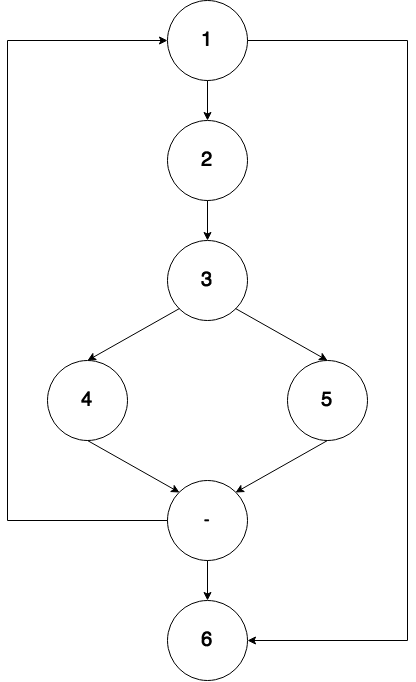
\includegraphics[width=0.7\textwidth]{CFG_Example.png}
\end{minipage}
\end{center}
\begin{center}
\noindent
\begin{minipage}{15em}
\begin{flushleft}
\noindent
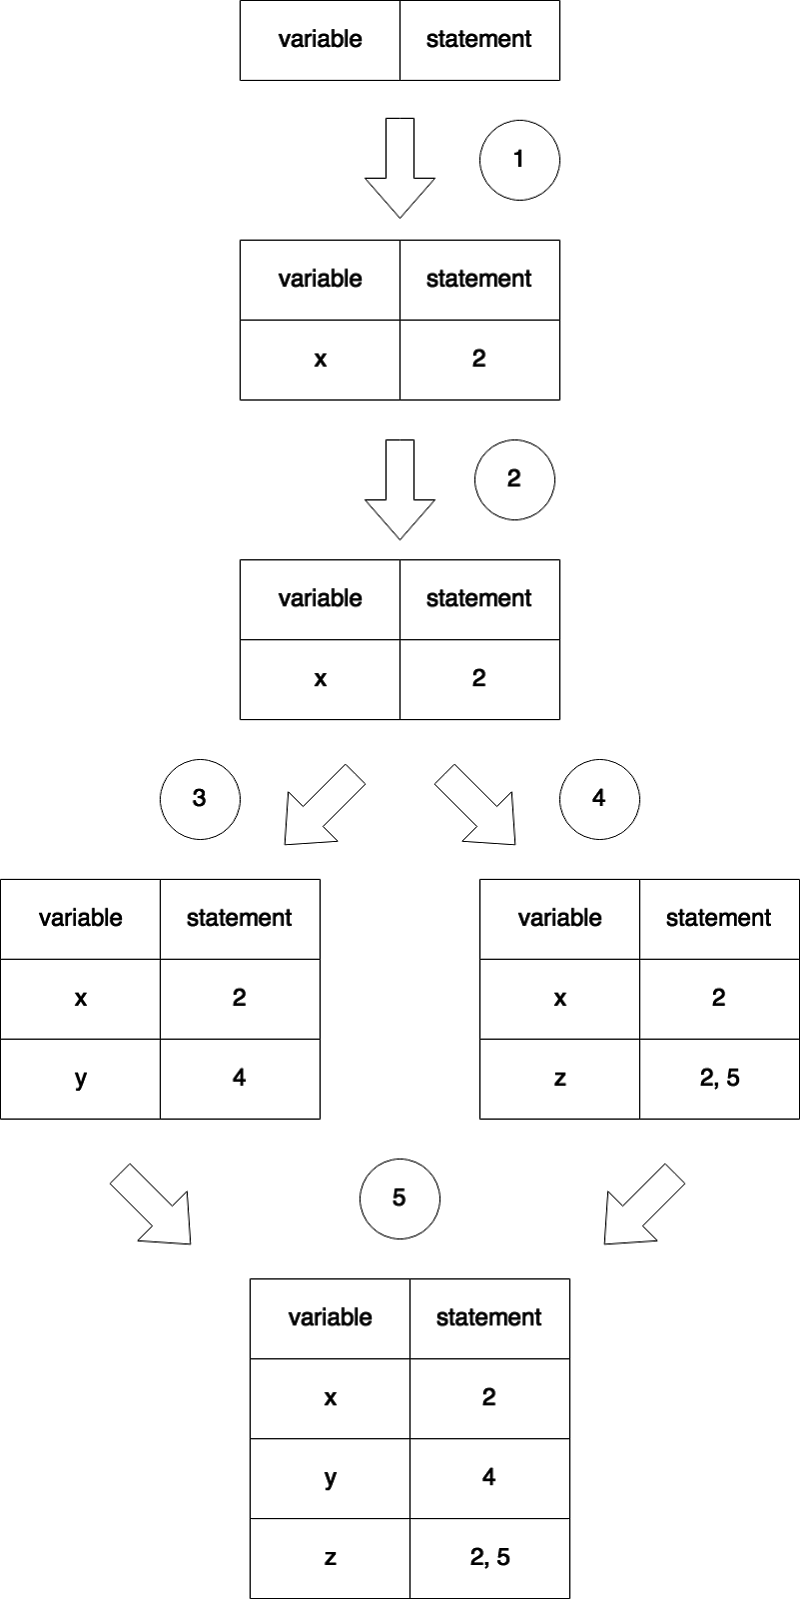
\includegraphics[width=1.15\textwidth]{affects1.png}
\end{flushleft}
\end{minipage}
\hspace{20mm}
\begin{minipage}{20em}
\normalsize
At the start, the \textbf{latestModifiedMap} is empty. As \textbf{stmt 1} is a while loop, we push the empty \textbf{latestModifiedMap} into the \textbf{whileMapStack}.
\begin{enumerate}
\item Stmt 2 uses \textbf{y}, but the \textbf{var y} is not in the latestModifiedMap, so we continue and put the \textbf{relation x} modified by stmt 2. (directly/indirectly) into the map.
\item As this is an if-statement, we branch out into arrows 3 and 4, making a copy of the current map as we iterate the if-else block.
\item We iterate the if block. Since \textbf{y uses z},which does not exist in the \textbf{latestModifiedMap}, we simply put the relation \textbf{y} modified by stmt 4 (directly/indirectly) into the map.
\item We now iterate the else block. Since stmt 5 uses \textbf{x} and \textbf{z} is affected by \textbf{x} which exists in the \textbf{latestModifiedMap}, we add the statements that modify z (directly/indirectly) into the map for var z. We also \textbf{add the affects* relation (2, 5)} into the cache. We then put the current statement, 5, as modifying z into the mapping from z.
\item At step 5, we have already finished iterating the if-else block and now merge the 2 separate \textbf{latestModifiedMaps} together. Since the merged map is different from the map we started with (the map on the \textbf{whileMapStack}), we have to continue to iterate the while loop until there are no new changes.
\end{enumerate}
\end{minipage}
\end{center}
\normalsize




\begin{center}
\noindent
\begin{minipage}{15em}
\begin{flushleft}
\noindent
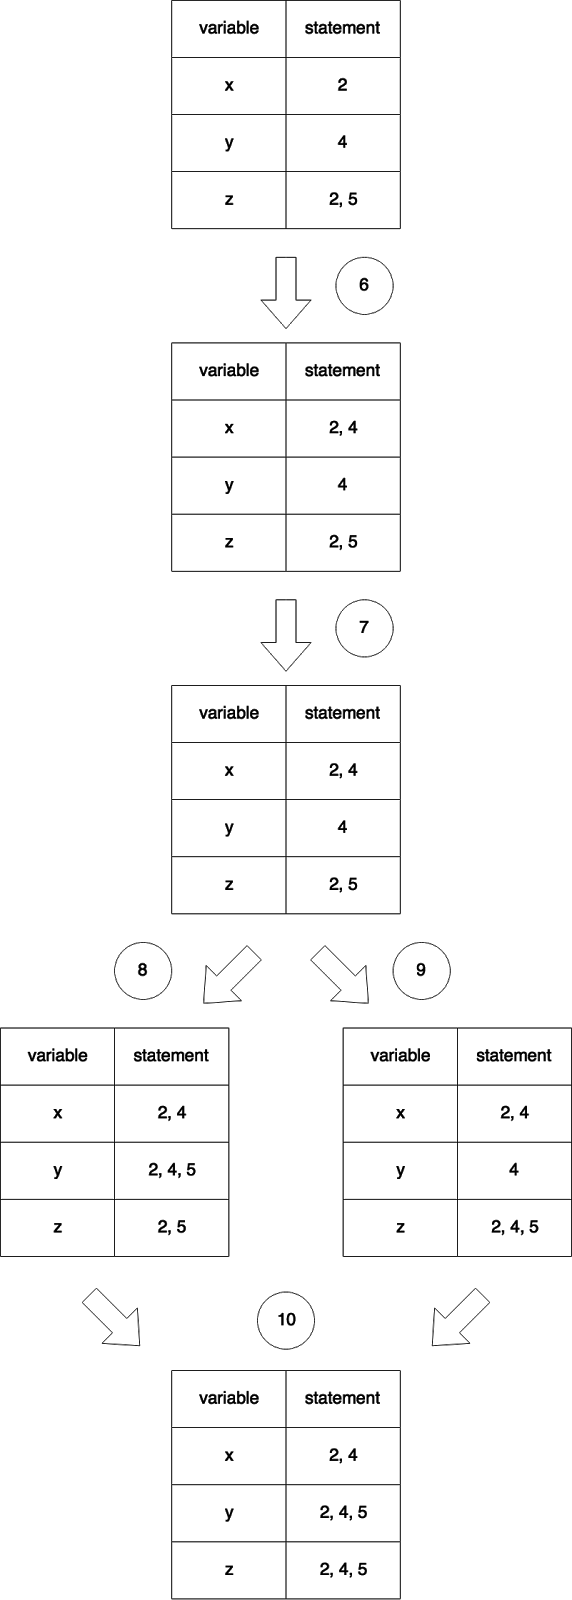
\includegraphics[width=1.15\textwidth]{affects2.png}
\end{flushleft}
\end{minipage}
\hspace{20mm}
\begin{minipage}{20em}
\normalsize
We iterate the while loop again with the latestModifiedMap generated from merging at step 5.
\begin{enumerate}
 \setcounter{enumi}{5}
\item We proceed into the while loop at statement 2. Since statement 2 uses y and y exists in the map, we \textbf{add the affects* relation (4, 2)} into the cache. At the same time, the statement 4 will be added to the set mapped from variable x.
\item We branch out at statement 3 is an if statement, making a copy of the latestModifiedMap for our use in the if and else branch.
\item Since statement 4 uses z and z exists in the map, we \textbf{add the affects* relation (2, 4) and (5, 4)} into the cache. We then also add statements 2 and 5 into the set being mapped from variable y.
\item Since statement 5 uses x and x exists in the map, we \textbf{add the affects* relations (2, 5) and (4, 5)} into the cache. We then also add statements 2 and 4 into the set being mapped from variable z.
\item As we have finished iterating through the if and else block, we merge the two maps from each path. We then compare the merged map with the map on the whileMapStack, in this was is the map before step 6. Since the maps are still different, this means that we have to iterate the while loop again.
\end{enumerate}
\end{minipage}
\end{center}
\normalsize


\begin{center}
\noindent
\begin{minipage}{15em}
\begin{flushleft}
\noindent
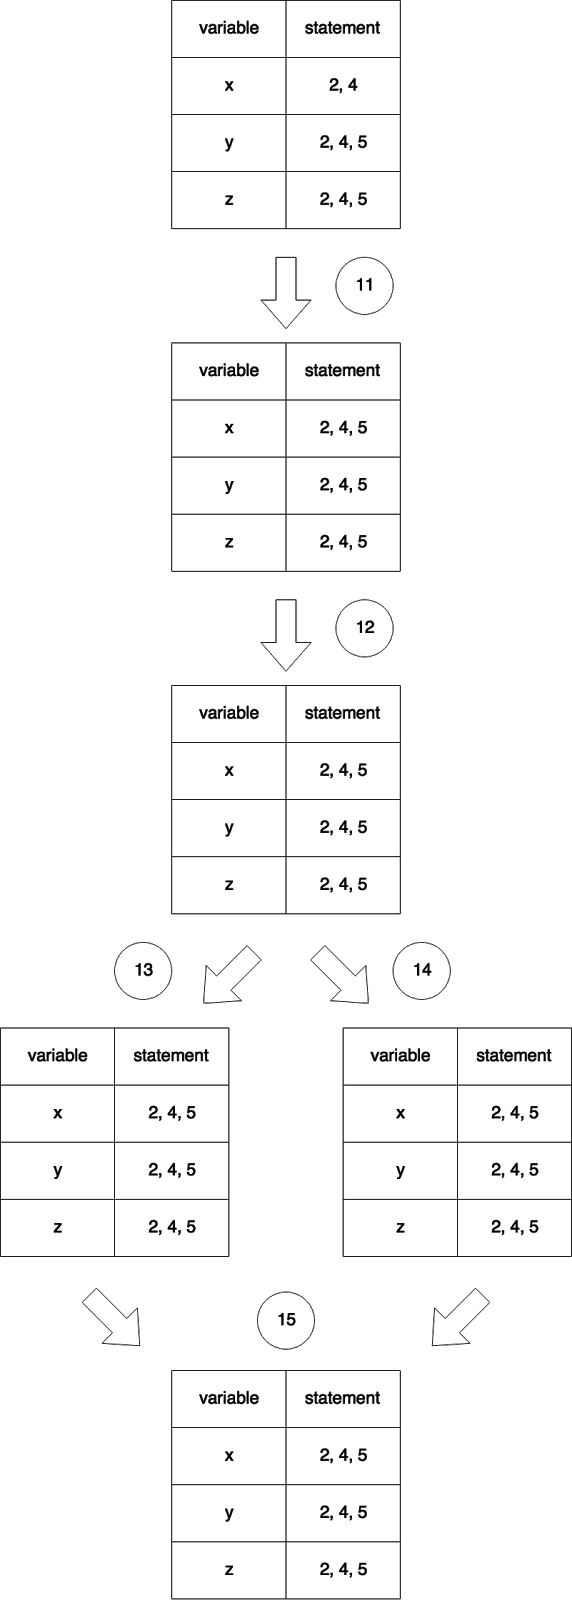
\includegraphics[width=1.15\textwidth]{affects3.png}
\end{flushleft}
\end{minipage}
\hspace{20mm}
\begin{minipage}{20em}
\normalsize
We iterate the while loop again with the new latestModifiedMap generated from the merging at step 10.
\begin{enumerate}
 \setcounter{enumi}{10}
\item We go on to statement 2 where y is being used. We then \textbf{add the affects* relations (2, 2), (4, 2), (5, 2)} into the cache. We then add the additional statements that directly/indirectly modified x into the map.
\item Once again, as statement 3 is an if statement, we make a copy of the latestModifiedMap and branch them out when we iterate the if and else block.
\item As statement 4 uses variable z, we \textbf{add the affects* relations (2, 4), (4, 4) and (5, 4)} into the cache. Then we update the set mapped from y accordingly.
\item As statement 5 uses variable x, we \textbf{add the affects* relations (2, 5), (4, 5) and (5, 5)} into the cache. Then we update the set mapped from z accordingly. 
\item We merge the 2 maps from if branch and else branch at this point. We then compare the map with the map we entered the loop with. As they were changes made, we have to iterate the while loop one more time.
\end{enumerate}
\end{minipage}
\end{center}
\normalsize


\begin{center}
\noindent
\begin{minipage}{15em}
\begin{flushleft}
\noindent
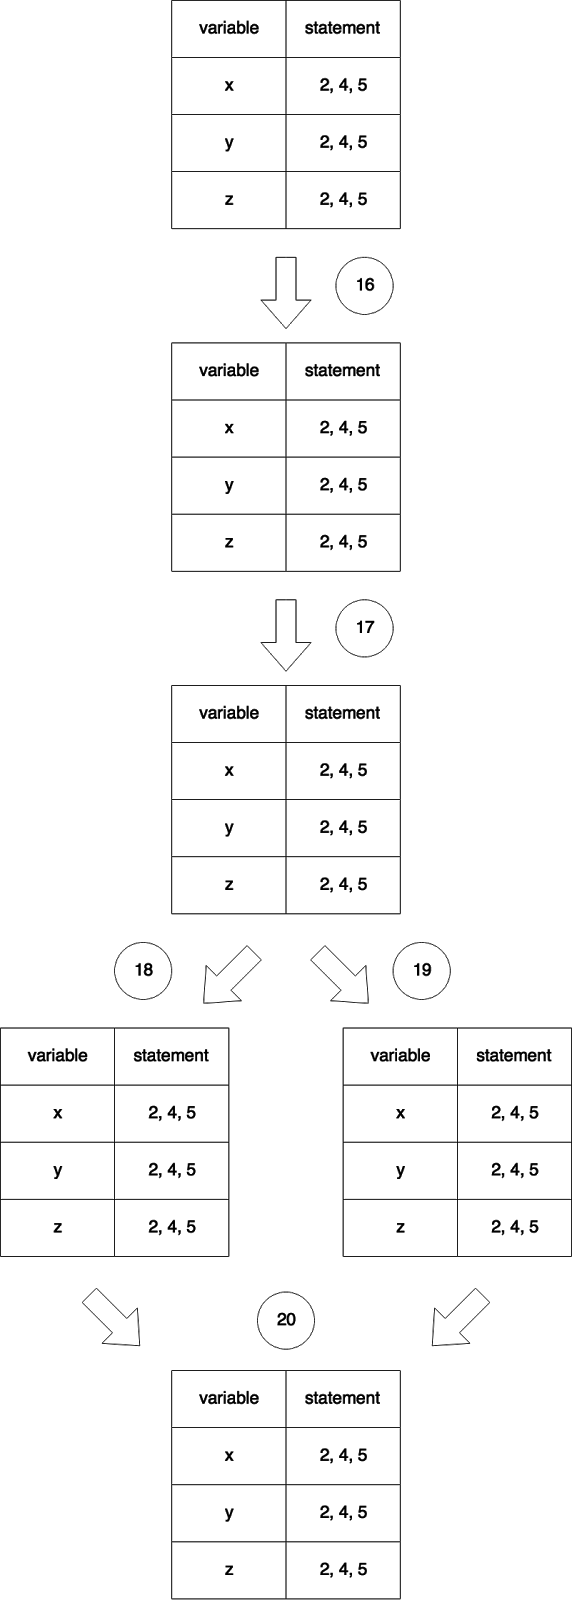
\includegraphics[width=1.15\textwidth]{affects4.png}
\end{flushleft}
\end{minipage}
\hspace{20mm}
\begin{minipage}{20em}
\normalsize
We iterate the while loop again with the new latestModifiedMap generated from the merging at step 15.
\begin{enumerate}
 \setcounter{enumi}{15}
\item We go on to statement 2 where y is being used. We then \textbf{add the affects* relations (2, 2), (4, 2), (5, 2)} into the cache. We then add the additional statements that directly/indirectly modified x into the map.
\item Once again, as statement 3 is an if statement, we make a copy of the latestModifiedMap and branch them out when we iterate the if and else block.
\item As statement 4 uses variable z, we \textbf{add the affects* relations (2, 4), (4, 4) and (5, 4)} into the cache. Then we update the set mapped from y accordingly.
\item As statement 5 uses variable x, we \textbf{add the affects* relations (2, 5), (4, 5) and (5, 5)} into the cache. Then we update the set mapped from z accordingly. 
\item We merge the 2 maps from if branch and else branch at this point. We then compare the map with the map we entered the loop with. Since the maps are now the same which means that we have captured all relations inside the while loop and updated the map accordingly, we can now exit the while loop and proceed to the statement after it, statement 6.
\end{enumerate}
\end{minipage}
\end{center}
\normalsize


\begin{center}
\noindent
\begin{minipage}{18em}
\begin{flushleft}
\noindent
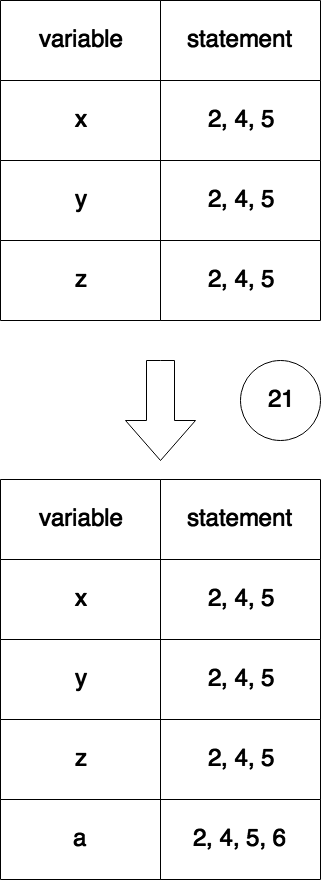
\includegraphics[width=0.5\textwidth]{affects5.png}
\end{flushleft}
\end{minipage}
\begin{minipage}{20em}
\normalsize
\begin{enumerate}
 \setcounter{enumi}{20}
\item At statement 6, since 6 uses x, we \textbf{add the affects* relations (2,6), (4, 6), (5, 6)} into the cache. At the same time, we update the variable modified, a, with the statements that directly/indirectly modifies the variables used.
\end{enumerate}
With this, we have finished extracting all the affects* relations in procedure Example. If there are more procedures, we will continue to do so with them. As noted above, there might be instances where we add duplicate affects* relations into our cache. The cache will be able to detect duplicates and remove them accordingly in order to be memory efficient.
\newline \newline
The final \textbf{Affects* relations} found in the cache are as follows: \newline
\textbf{(2, 2), (2, 4), (2, 5), (2, 6), (4, 2), (4, 4), (4, 5), (4, 6), (5, 2), (5, 4), (5, 5), (5, 6)}.

\end{minipage}
\end{center}
\normalsize



\subsubsection{Design Extractor}} 
The role of the Design Extractor is to compute the complex relations from the tables that Parser has populated. It computes Parent*, Follows* and Calls* relations as well as the interprocedural Uses/Modifies relations. The Parser will call upon the Design Extractor to process these relations once it is done with parsing the SIMPLE source code. \vspace{4mm}\newline
\textbf{\underline{Computation of Parent*/Follows*/Calls* relations}}\newline
The computation of these complex relations are relatively similar and use the same algorithm. The Design Extractor iterates through the respective base tables (e.g. ParentsTable, FollowsTable) and appends the information found in these tables to the current list.
\begin{figure}[htbp]
  \caption{Parent to Child/ChildStar Table}
  \centering  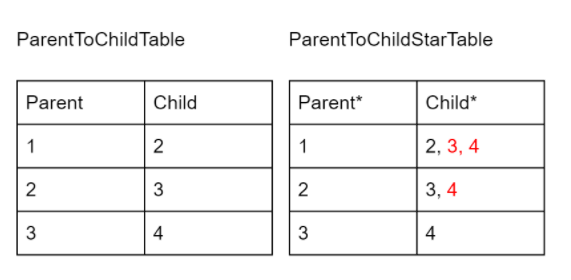
\includegraphics[width=0.5\textwidth]{ParentTable1.png}
\end{figure}
Using the computation of Parent* relations from the Parent relations table given in Fig.4 as an example, starting from statement 1, as the relation Parent(1, 2) is true, we then check if statement 2 is a parent statement. In this case, Parents(2, 3) exists, so 3 is appended onto the list of Child* in the ParentToChildStarTable[1]. We then continue to check the child of the current statement (in this case, statement 2) to see if it has a child statement. Since the relation Parent(3, 4) exists, we continue to append 4 onto ParentToChildStarTable[1]. Next, we check if statement 4 is a parent of any statement. Since there does not exist a child with statement 4 as its parent, all the Children* relationship for statement 1 has been computed. We then continue the same steps for all Parents in the ParentToChildTable. \newline
\begin{figure}[htbp]
  \caption{Child to Parent/ParentStar Table}
  \centering  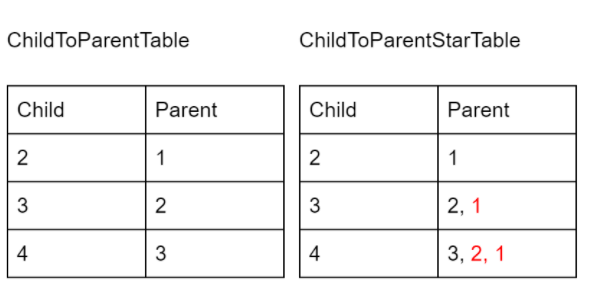
\includegraphics[width=0.5\textwidth]{ParentTable2.png}
\end{figure}
\vspace{4mm}
The reverse relations e.g. ChildToParentStarTable given in Fig.5 is also computed in the Design Extractor to facilitate faster result selection.

Similar to Parent and Parent* relations, Follows/Follows* and Calls/Calls* relations can be computed in the same manner.

\textbf{\underline{Computation of Inter-Procedural Uses/Modifies}}\newline
Computing Uses and Modifies relations that involve procedures requires a traversal of the Calls graph. Our Calls graph is essentially the table of Calls relationship, which acts as an adjacency list.The Design Extractor does a depth first search to reach the leaf nodes and propagate upwards in post-order fashion.
The Design Extractor iterates through every Caller procedure and starts a DFS from it. In a Calls graph, the arrow is directed from a Caller to a Callee (i.e. Calls(A, B)). 
\newline In this example, we will start the DFS from procedure A. 
\begin{figure}[h]
  \caption{Call Traversal from Proc A}
  \centering  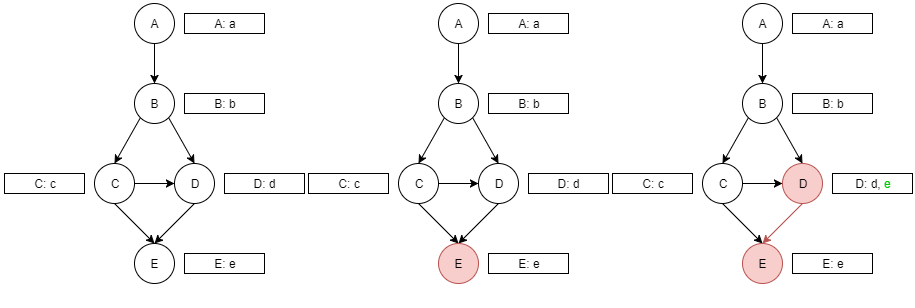
\includegraphics[width=1.0\textwidth]{Call_Traversal.png}
\end{figure}
\vspace{4mm} \newline
From A, it will traverse down until procedure E and mark it as visited (highlighted in red). As E is a leaf node, it means that it does not call any procedures hence there are no new additional variables appended to its list of variables used. Once visited, it will reverse back to it’s parent, in this case procedure D. The Design Extractor then checks if all the procedures called by D have been visited. In this case, it is only E that is visited, and hence it appends the variables that E uses onto its list of variables used (in green).
\begin{figure}[h]
  \caption{Call Traversal from Proc A}
  \centering   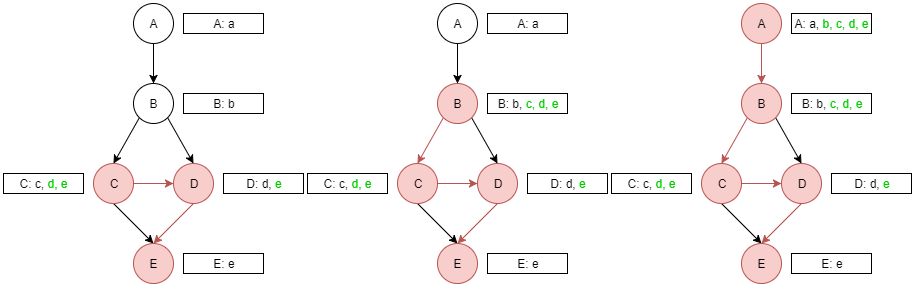
\includegraphics[width=1.0\textwidth]{Call_Traversal_2.png}
\end{figure}
\newline From D, it returns back to its caller C. C checks if all its callees have been visited and if so, appends their used variables onto its list. If its callee’s nodes are not visited yet, we run the DFS on the callee. We do so until we return to node A, the node that we started with for this example.

The reason why this algorithm is run on every caller procedure is to ensure complete coverage of all Uses in the case where there could be multiple disjoint calls graphs. The same algorithm is run to compute inter-procedural Modifies relations.
\vspace{4mm}\newline
\textbf{\underline{Computation of Container Statement Uses/Modifies}}\newline
After the population of inter-procedural modifies relations, we can then compute Uses and Modifies relations for container statements that contain a call statement in their statement list.

The Design Extractor will retrieve all the Call statements and find the list of Parent* of it. For each Parent*, it will sent that Parent*’s statement to use the variables that are used by the procedure of the Call statement. \newline Consider the following source code
\begin{center}
\fbox{\begin{minipage}{35em}
\texttt{procedure A \{
\newline1 \hspace{3mm}	while a \{
\newline2 \hspace{10mm}	while c \{
\newline3 \hspace{17mm} call B;
\newline \hphantom{he} \hspace{15mm} \}
\newline \hphantom{he} \hspace{7mm}		\}
\newline 	\}
\newline procedure B \{
\newline4 \hspace{3mm}  x = a + b + c;
\newline \}}
\end{minipage}}
\end{center}
\vspace{10mm}
The Design Extractor will get the list of call statements, in this case only statement number 3. Then, it will get all the Parent* of statement 3 which are \{2, 1\}. For all the Parent* statements, \{2, 1\}, their use relations would be updated with the variables used by statement 3, \{a, b, c\}.
\begin{figure}[htbp]
  \caption{Statement to Variable Tables}
  \centering  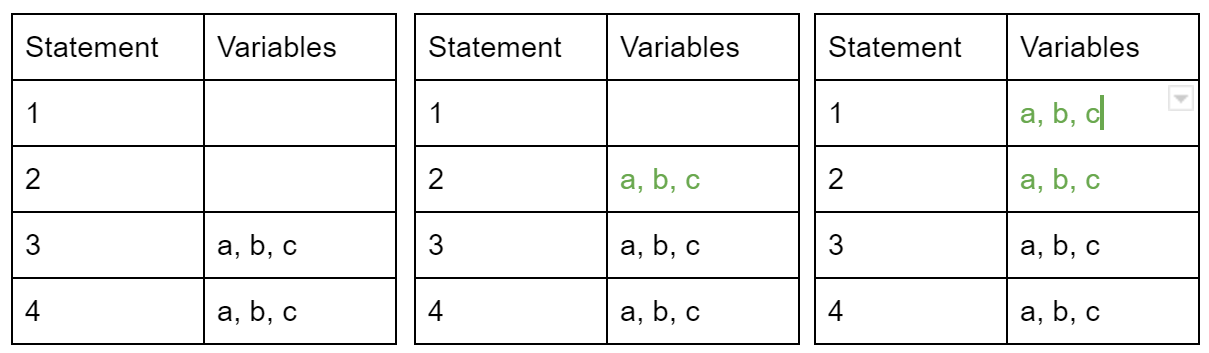
\includegraphics[width=0.9\textwidth]{uses_propagating.png}
\end{figure}
\vspace{4mm}

The same idea used in computing Uses relation and Modifies relation for container statements.

\subsubsection{PQLMain}
The PQLMain is the main class that other components interact with. PQLMain employs the \textbf{Facade} pattern, whereby other components that need to use PQLMain do not need to know the implementations and the sub-components inside PQLMain. When it is initialised, it takes in a query string and instantiates a blank QueryTree (the main storage component) which is used throughout the process of  query processing and evaluation. Fig.9 shows the component diagram of the PQLMain and its sub-components. \newline
\begin{figure}[H]
  \caption{PQLMain Facade Component diagram}
  \centering 
 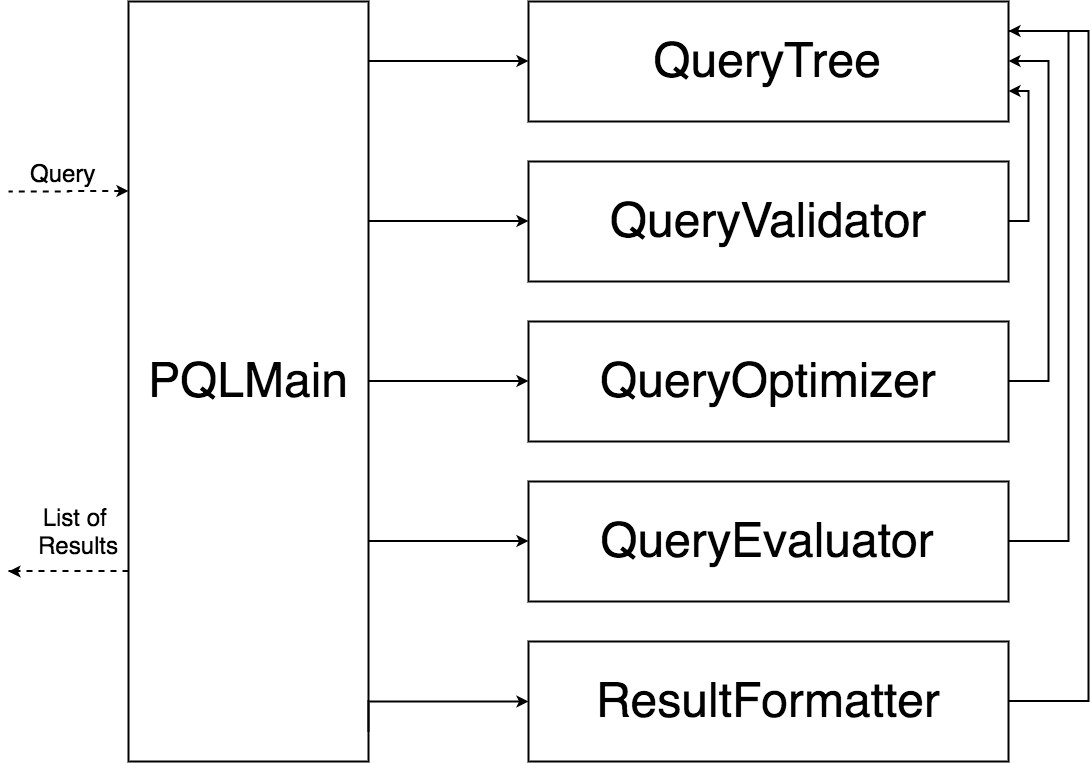
\includegraphics[width=0.5\textwidth]{PQLComponents.jpg}
\end{figure}
\subsubsection{Query Validator}
The QueryValidator ensures that the query received from PQLMain is syntactically and semantically correct. A series of validation steps are executed while parsing the query to check whether the structure of the query is well-formed and whether the arguments of each individual clause are declared and consist of permitted argument types as described in the program design model. It relies heavily on regular expressions (Regex) that are aligned to the PQL grammar. As the QueryValidator performs its validation routine, it also helps to build an internal storage structure, the QueryTree, by storing only essential parts of the query. This watered-down version of the query will ease the work of the QueryEvaluator. \newline
The steps parsing the query (given below) are as follows:
\begin{center}
\fbox{\begin{minipage}{40em}
\begin{flushleft}stmt s; assign a, a1  , a2;
\newline Select s such that Follows (s, a) pattern a(\_, \_) with a.stmt\# = s.stmt\#
\end{flushleft}
\end{minipage}}
\end{center}
\vspace{4mm}
\begin{enumerate}
\item Upon receiving a query from PQLMain, the QueryValidator will attempt to dissect the query into Declaration and Selection. This can be done by splitting the query with semi-colons as the delimiter. As each valid query will have its Selection as the last token, any token before the last will be considered as Declaration.
\begin{figure}[H]
  \caption{State of query after dissection}
  \centering 
 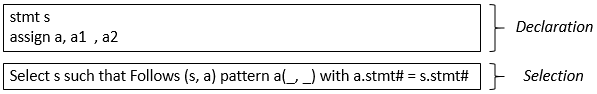
\includegraphics[width=0.8\textwidth]{DissectedQuery.png}
\end{figure}
\item The QueryValidator uses regex to extract and validate the declaration entities and synonyms. 
The QueryValidator will split the declaration into the entity token and synonym token.
The first sub-token will be compared against the acceptable entity as defined in the PQL grammar. If it is invalid, the QueryValidator will immediately return false. If it is valid, it proceeds, and for all subsequent sub-tokens, if any of them are invalid, the QueryValidator will return false. 
Validation proceeds similarly for synonym tokens.
If the entire declaration is valid, the entire declaration is stored in the QueryTree.
Do note that we do not allow duplicate declarations. 

For example, \begin{verbatim}
stmt s; stmt s;
Select s

stmt s, s;
Select s
\end{verbatim}
are considered invalid.
\item After processing Declaration, the QueryValidator will compare Selection against the overall regex definition derived from the PQL grammar. This regex picks up clause group as shown below
\begin{figure}[H]
  \centering 
 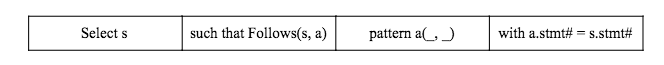
\includegraphics[width=0.7\textwidth]{Step3.png}
\end{figure}
\item With the query being partitioned into distinctive clauses, the QueryValidator validates each clause independently. For each clause, the QueryValidator passes it to SelectionValidator. As the query has already passed the overall regex check, there is no need to look for clause keywords to determine which clause they belong to, hence clause keywords (‘select’, ‘such that’, ‘pattern’, ‘with’ and ‘and’) can be dropped.
\begin{figure}[H]
  \centering 
  \caption{QueryValidator Selection: State of clause before SelectionValidator passes it to the respective handlers}
 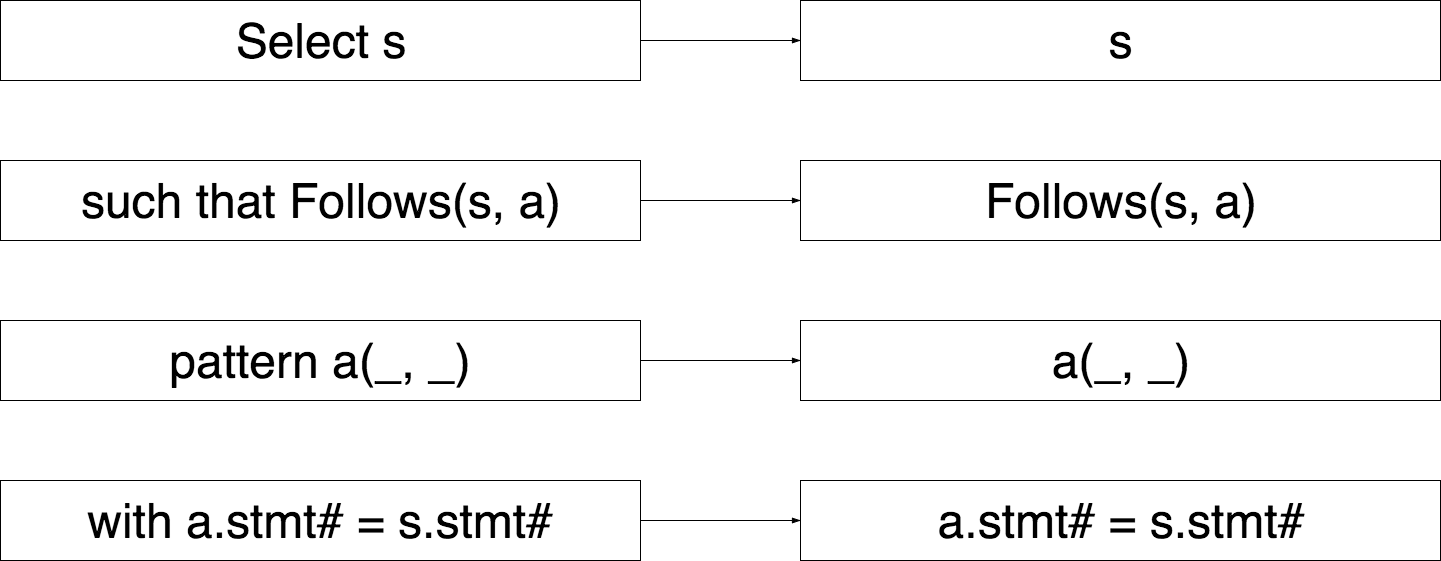
\includegraphics[width=0.7\textwidth]{QvSelection.png}
\end{figure}
\end{enumerate}
The SelectionValidator will then pass the processed clause to the respective clause handler that is supposed to handle that type of clause. The Handler will then delegate the respective sub-validators to validate and extract the arguments and types of argument. The Handlers adopts the \textbf{Strategy} pattern to determine which sub-validator to pass the clause to.
\begin{figure}[H]
  \centering 
  \caption{QueryValidator Handler: Possible path taken}
 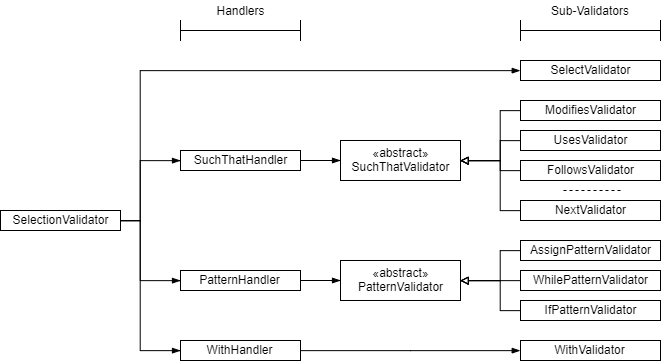
\includegraphics[width=1.0\textwidth]{QVHandler.png}
\end{figure}
Each sub-validator extracts the argument and enquires the QueryTree for the type of argument. Once the sub-validator receives the information from the QueryTree, it will tag each argument to its appropriate type.

Arguments are tagged according to their entity type, specific to their respective clauses. The tagging system makes use of enums. \newline
\begin{table}[H]
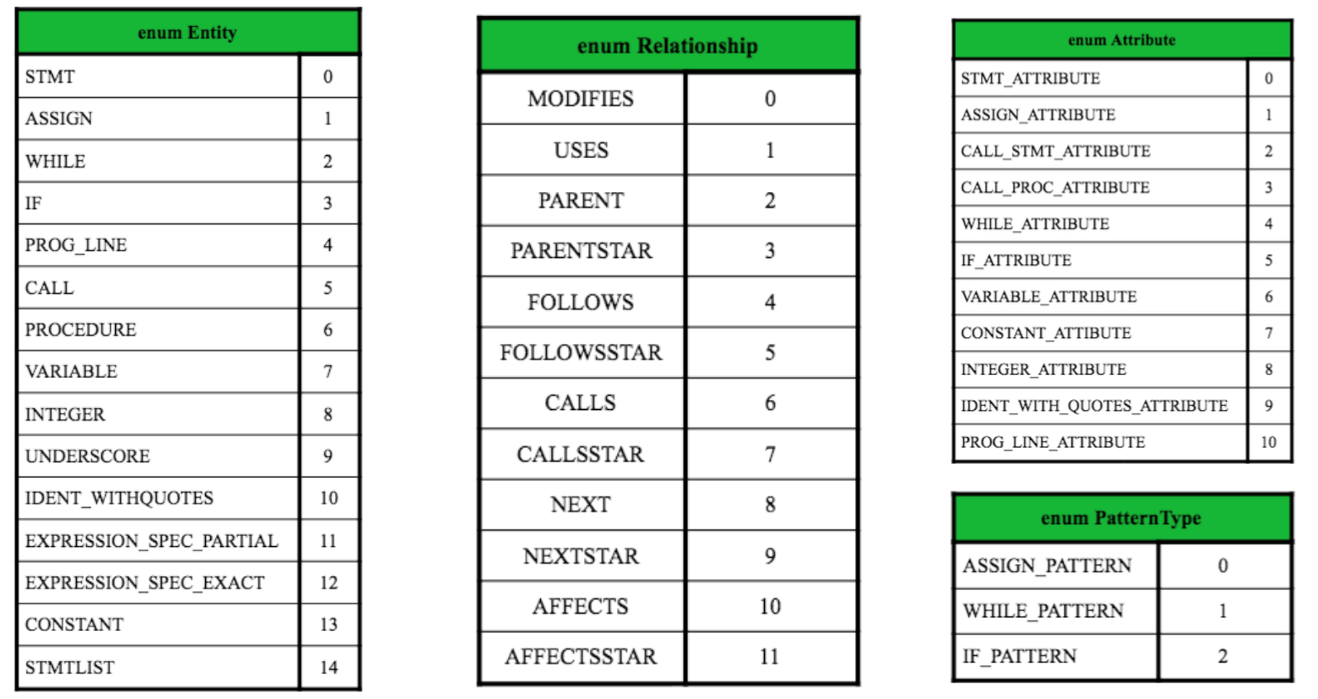
\includegraphics[width=1.0\textwidth]{Enums.png}
\caption{Enums}
\end{table}
Do note that due to ambiguity in the detection of \textbf{Select BOOLEAN} in an invalid query, we will return \textit{false} whenever we detect BOOLEAN in a query.

For example:
\begin{verbatim}
Select BOOLEAN hello
\end{verbatim}
returns false.

For Iteration 3, we have extended our SPA to validate \textbf{Select tuples} and Select synonyms with \textbf{attributes}. 

For attribute validation, we use regex to split the synonym into synonym and attribute. We first validate the synonym syntactically. Then we proceed with semantic validation for its corresponding attribute type. Here, since CALL entity can have two attributes - procName and stmt\# - we also store an additional flag in the QueryTree to let the ResultFormatter know whether to get the string mapping from PKB for CALL when projecting results to the UI.

For tuple validation, we extract each tuple argument and proceed to validate it as we would validate each synonym, and store it in the QueryTree.

\begin{comment}
\begin{table}
\centering
\begin{tabular}{|c|c|}
\hline
\cellcolor{green!35}Enum Relationship & \cellcolor{green!35}Value \\\hline
MODIFIES & 0 \\\hline
USES & 1 \\\hline
PARENTS & 2 \\\hline
PARENTSTAR & 2 \\\hline
FOLLOWS & 3 \\\hline
FOLLOWSSTAR & 4 \\\hline
CALLS & 5 \\\hline
CALLSSTAR & 6 \\\hline
NEXT & 7 \\\hline
NEXTSTAR & 8 \\\hline
AFFECTS & 10 \\\hline
AFFECTSSTAR & 11  \\\hline
\end{tabular}
\caption{\label{Relationship Enum}
\end{table}
\begin{table}[htbp]
  \caption{Entity Enum}
 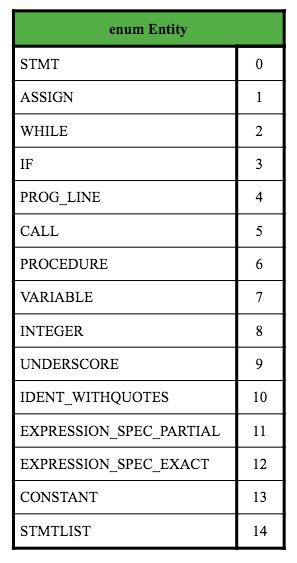
\includegraphics[width=0.3\textwidth]{EnumEntity.png}
\end{table}
\end{comment}
\begin{figure}[H]
  \caption{Query Validation Handler}
 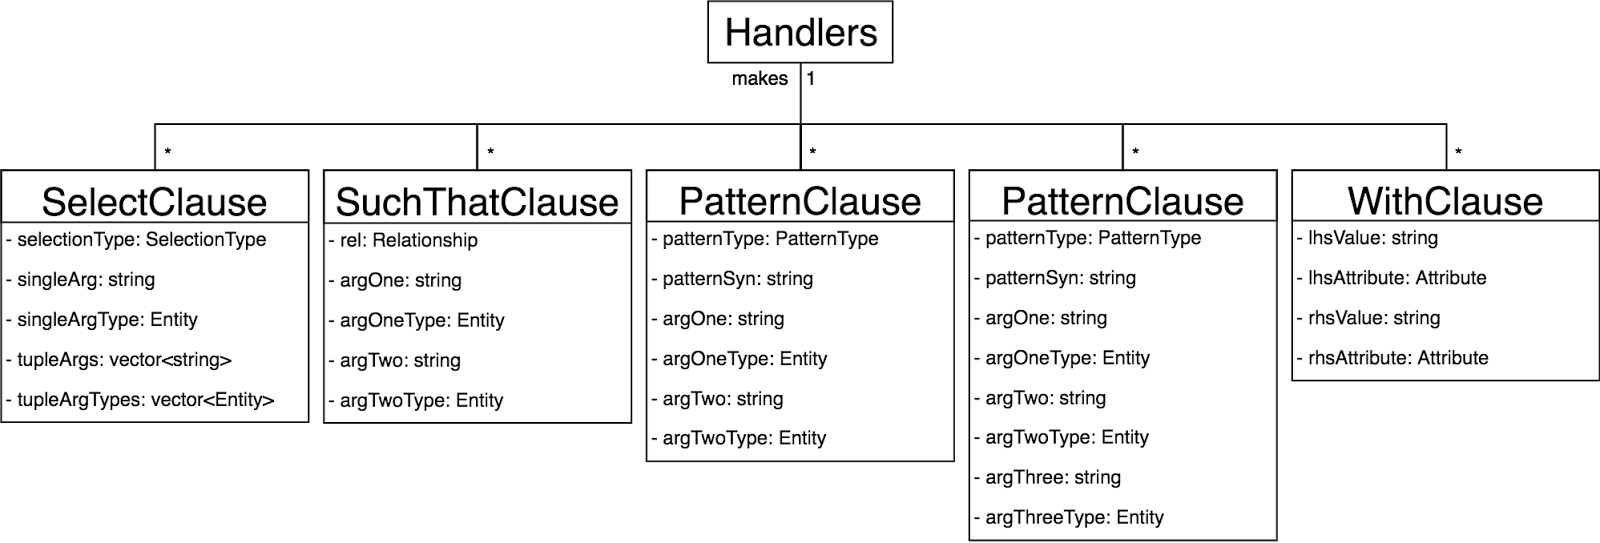
\includegraphics[width=1.1\textwidth]{ClauseInteraction.png}
\end{figure}
Upon validation and extraction, the sub-validators will return their results to the Handler. The generation of ClauseObject is done via the Factory pattern, using the information retrieved from each sub-validatos. Handler will encapsulate this information into a ClauseObject before storing it in the QueryTree.

The decision making at each stage is shown below.
\begin{figure}[H]
  \centering 
  \caption{Validator Flowchart}
 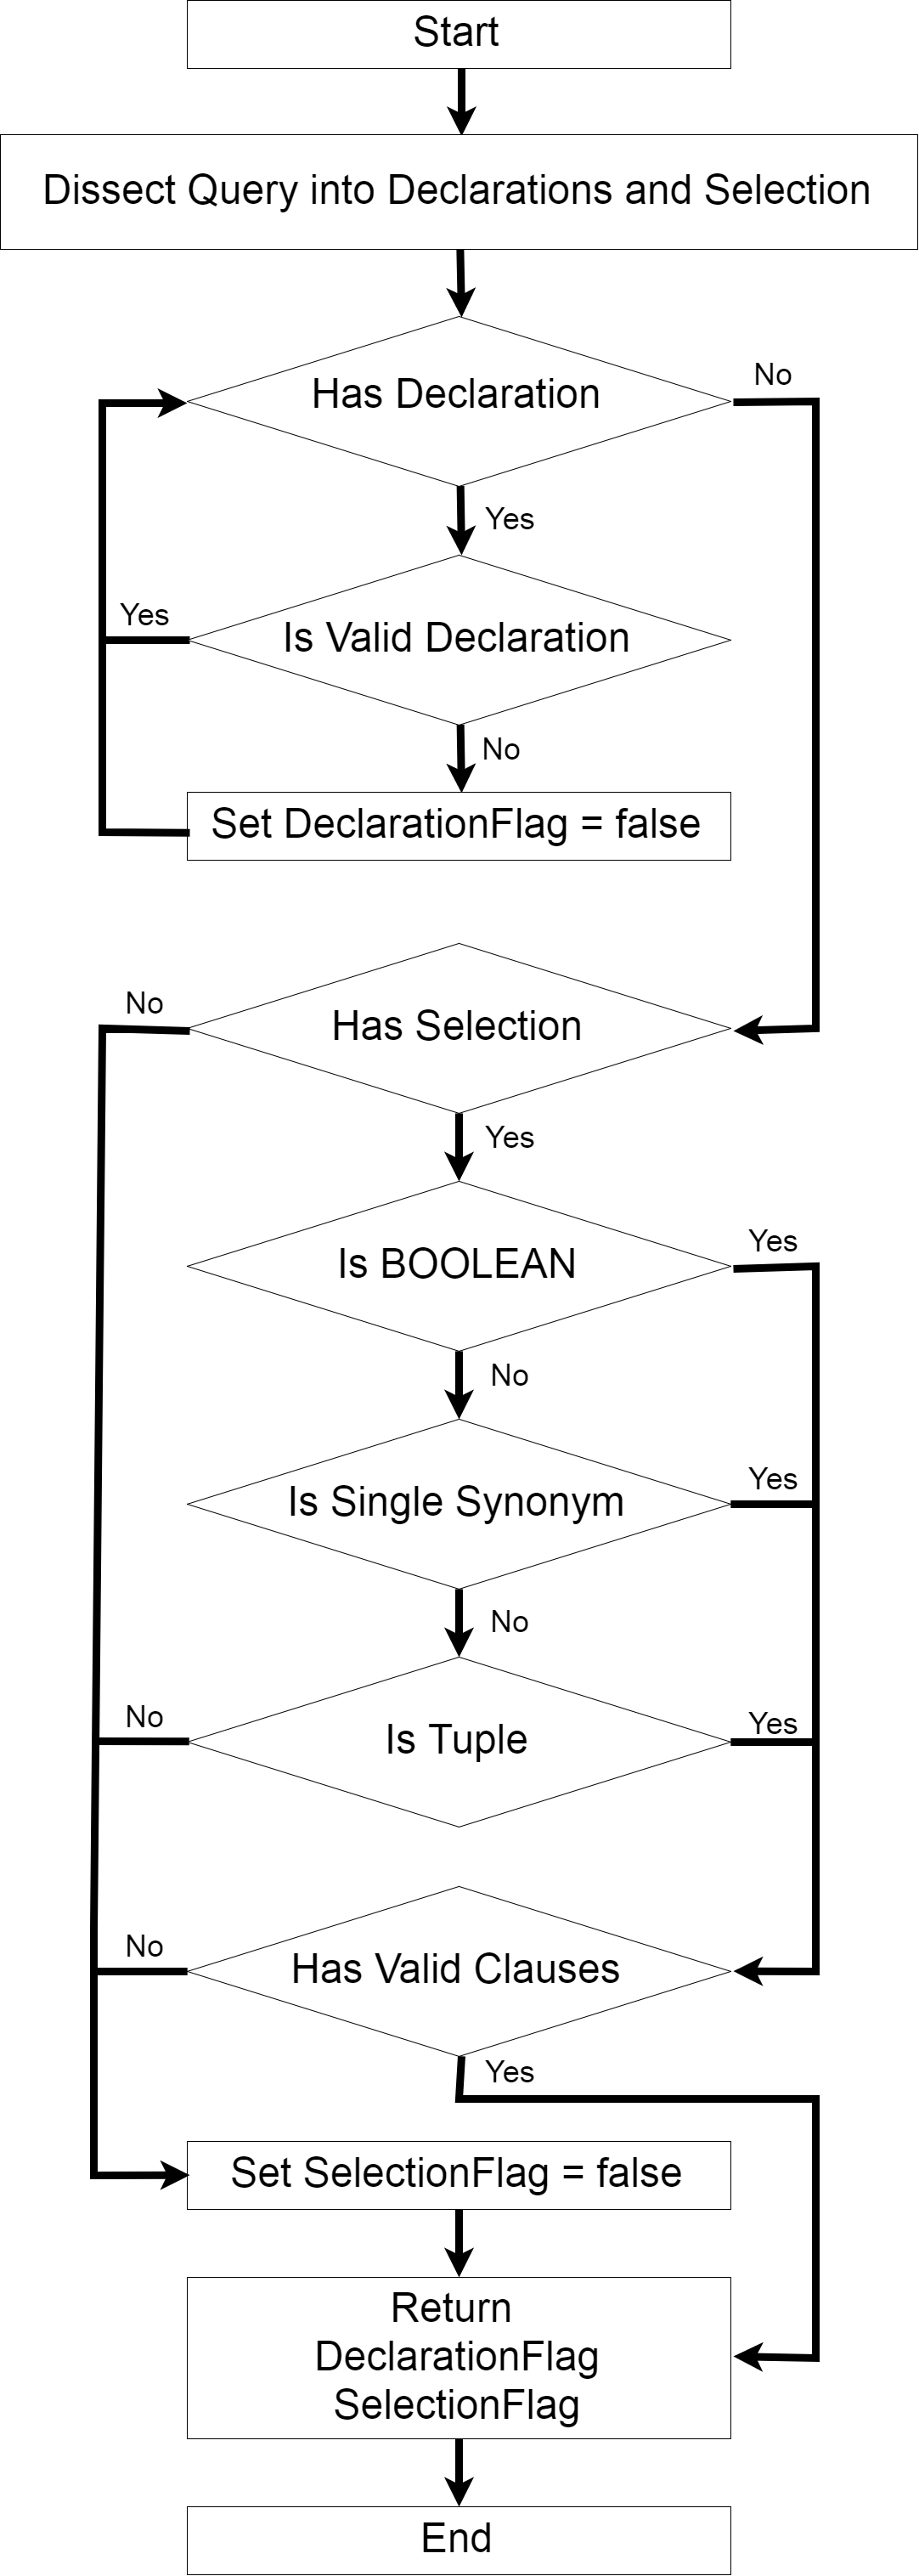
\includegraphics[width=0.5\textwidth]{QV_Flowchart.png}
\end{figure}
\subsubsection{Query Optimiser}
The QueryOptimiser is designed to pre-process the clauses in a query and perform optimisation such that inefficient evaluation of the query clauses is avoided and near optimal evaluation time can be achieved by the QueryEvaluator. After being created by the QueryValidator, the QueryTree is passed to the QueryOptimiser before it is passed to the QueryEvaluator for evaluation.
\newline
First and foremost, QueryOptimiser will perform some basic pre-processing. Duplicate clauses are removed, and when there are with-clauses with ident, overwriting of synonyms is also done.
\newline For example: \newline
\begin{center}
\fbox{\begin{minipage}{40em}
\texttt{procedure p; stmt s; \newline
Select s such that Uses(p,“x”) with p.procName = “funProcedure”}

Uses-clause will be modified to Users(funProcedure, “x”) and the with-clause will be removed from the queryTree.

\end{minipage}}
\end{center}

The QueryOptimiser then groups and reorders the QueryTree based on the following heuristics:
\begin{enumerate}
\item Avoid cross-products with synonyms not already present in intermediate table
\item The more synonyms present in the intermediate result table, the larger it is likely to become
\item The larger the results of a clause, the more time-consuming cross-product operation it’ll likely cause in the future
\item With-clauses and pattern-clauses yield very small sets of results, therefore they should be prioritised
\item Compute Next, Next*, Affects and Affects* at the end
\item Overwriting synonyms whenever possible (using With clauses with ident)
\item Select-clause can result in very big intermediate results if the query is selecting tuple with many synonyms that are not present in other clauses
\end{enumerate}

Most of the heuristics above aim to minimise number of cross-products, minimise the intermediate result size (to lower the cost of cross-product), and evaluate clauses that need to be computed during runtime only after the cheaper clauses are evaluated.

One strategy used to extract all the clauses in the QueryTree and split them into various clause groups is based on the common synonyms they have. The grouping is done such that all synonyms only belong to only one group, and each synonyms in a clause group is “linked” to every other synonyms in the same clause group by at least one clause. A synonym is said to be “linked” to another synonym if both of them exist as arguments in a clause, e.g. “a1” is linked to “v1” by the clause Modifies(a1, v1).

In addition, the Optimiser also stores a table that assigns an estimated cost to each type of clause. SpaXI’s Optimiser estimates the cost of clauses based on statistical estimation and heuristics, as well as the size of the result. \newline
\begin{center}
\textbf{\textit{Cost = Number of Computations (PKB) + Result Size}}
\end{center}

The result size of a clause is as important as computation time because the size of the result will influence the time taken of cross-product in the intermediate result.

This table lists the summary of the costs allocated to each clauses, sorted in ascending order, for a source code with 500 statements. \newline
\begin{center}
\begin{longtable}{ |c|c|c|c| }
\hline
\textbf{ Clause Type}	 & \textbf{Cost} & \textbf{Worst-case time comlpexity} & \textbf{Result size}\\ \hline
\footnotesize
WITH\_ANY\_ARGS&0&-&0\\\hline
FOLLOWS\_BOOLEAN&1&$O(1)$&0\\\hline
NEXT\_BOOLEAN&1&$O(1)$&0\\\hline
CALLS\_BOOLEAN&1&$O(1)$&0\\\hline
PARENT\_BOOLEAN&1&$O(1)$&0\\\hline
CALLS\_STAR\_BOOLEAN&1&$O(1)$&0\\\hline
PARENT\_STAR\_BOOLEAN&1&$O(1)$&0\\\hline
MODIFIES\_BOOLEAN&1&$O(1)$&0\\\hline
USES\_BOOLEAN&1&$O(1)$&0\\\hline
FOLLOWS\_STAR\_BOOLEAN&1&$O(1)$&0\\\hline
FOLLOWS\_1ARG&2&$O(1)$&1\\\hline
NEXT\_1ARG&2&$O(1)$&1\\\hline
CALLS\_1ARG&11&$O(1)$&10\\\hline
CALLS\_STAR\_1ARG&31&$O(1)$&30\\\hline
CALLS\_2ARGS&121&$O(1)$&120\\\hline
CALLS\_STAR\_2ARGS&151&$O(1)$&150\\\hline
SELECT\_1ARG&501&$O(1)$&500\\\hline
PARENT\_1ARG&501&$O(N)$&1\\\hline
MODIFIES\_1ARG&525&$O(N)$&25\\\hline
USES\_1ARG&550&$O(N)$&50\\\hline
PATTERN\_1ARG&750&$O(N)$&250\\\hline
PARENT\_STAR\_1ARG&800&$O(N)$&300\\\hline
PATTERN\_2ARGS&1000&$O(N)$&500\\\hline
FOLLOWS\_STAR\_1ARG&1000&$O(N)$&500\\\hline
PARENT\_2ARGS&1000&$O(N)$&500\\\hline
FOLLOWS\_2ARGS&1000&$O(N)$&500\\\hline
NEXT\_2ARGS&1000&$O(N)$&500\\\hline
NEXT\_STAR\_BOOLEAN&1500&$O(V+E)$&0\\\hline
NEXT\_STAR\_1ARG&2000&$O(V+E)$&500\\\hline
PARENT\_STAR\_2ARGS&2000&$O(N)$&1500\\\hline
MODIFIES\_2ARGS&5500&$O(N)$&5000\\\hline
USES\_2ARGS&15500&$O(N)$&15000\\\hline
FOLLOWS\_STAR\_2ARGS&50500&$O(N)$&50000\\\hline
AFFECTS\_BOOLEAN&90000&$O(2*(V+E))$&0\\\hline
AFFECTS\_1ARG&90040&$O(2*(V+E))$&40\\\hline
NEXT\_STAR\_2ARGS&875000&$O(V*(V+E))$&125000\\\hline
AFFECTS\_STAR\_BOOLEAN&20833250&$N(N+1)(N+2)/6$&0\\\hline
AFFECTS\_STAR\_1ARG&20833350&$N(N+1)(N+2)/6$&100\\\hline
AFFECTS\_2ARGS&20843250&$N(N+1)(N+2)/6$&10000\\\hline
AFFECTS\_STAR\_2ARGS&20953250&$N(N+1)(N+2)/6$&120000\\\hline
SELECT\_TUPLE&INF&$-$&INF\\\hline
\end{longtable}
\end{center}
The following table gives a more comprehensive explanation of how the PKB computation cost is calculated. 
\begin{center}
\begin{longtable}{ |L{8cm} | L{9cm}| }
\hline
\textbf{ Clause Type} & \textbf{PKB Computation Time} 
(for 500 LoC SIMPLE source)  \\\hline
 WITH\_ANY\_ARGS & Always put as first clause based on the heuristic reasoning that with-clauses generally result in very small result size. The only exception is when there are two synonyms which are stmt.stmt\# and prog\_line.progline\#. But this happens very rarely and SpaXI ignores it.  \\\hline  
\newline
FOLLOWS\_BOOLEAN\newline
NEXT\_BOOLEAN\newline
CALLS\_BOOLEAN\newline
PARENT\_BOOLEAN\newline
CALLS\_STAR\_BOOLEAN\newline
PARENT\_STAR\_BOOLEAN\newline
MODIFIES\_BOOLEAN\newline
USES\_BOOLEAN\newline
FOLLOWS\_STAR\_BOOLEAN\newline
FOLLOWS\_1ARG\newline
NEXT\_1ARG\newline
CALLS\_1ARG\newline
CALLS\_STAR\_1ARG\newline
CALLS\_2ARGS\newline
CALLS\_STAR\_2ARGS\newline
SELECT\_1ARG\newline
 & Constant time as these data are stored using unordered\_map in PKB, $O(1)$
 \\\hline
\newline
NEXT\_STAR\_BOOLEAN\newline
NEXT\_STAR\_1ARG\newline
 & 
Breath-first search is performed on the CFG.
$O(V+E)$, where V and E are the number of vertices and edges in the CFG respectively.
Est: $V$ = 500; $E = 2 * V$
 \\\hline
\newline
PARENT\_STAR\_2ARGS\newline
MODIFIES\_2ARGS\newline
USES\_2ARGS\newline
FOLLOWS\_STAR\_2ARGS\newline
 & 
$O(N)$, $N$ = max num of stmts (sieving)
Est: $N$ = 500
 \\\hline
\newline
AFFECTS\_BOOLEAN\newline
AFFECTS\_1ARG\newline
 & 
2 times of Next* computation time
BFS is performed on CFG. For each vertex, check Uses relation. Complexity is $O(2*(V+E))$ * (avg num of used variables), where $V$ is the number of vertices and $E$ is the number of edges in the CFG.
Est: $V = 500; E = 2 * V$; avg used number of variable = 30
 \\\hline  
\newline
NEXT\_STAR\_2ARGS
\newline
 & 
$O(N)$, $N$ = max num of stmts (sieving)
Est: $N$ = 500
 \\\hline   
\newline
AFFECTS\_BOOLEAN\newline
AFFECTS\_1ARG\newline
 & 
Num of nodes x Complexity of Next*
BFS: $O(V*(V+E))$
Est: $V = 500; E = 2 * V$

 \\\hline  
\newline
AFFECTS\_STAR\_BOOLEAN\newline
AFFECTS\_STAR\_1ARG\newline
AFFECTS\_2ARGS\newline
AFFECTS\_STAR\_2ARGS\newline
 & 
Num of nodes x Complexity of Next*
BFS: $O(V*(V+E))$
Est: $V = 500; E = 2 * V$

 \\\hline 
\newline
SELECT\_TUPLE
\newline
 & 
$O(1*tupleSize)$
 \\\hline  
\end{longtable}
\end{center}

\normalsize

Clauses within all clause groups are then sorted based on the costs of each clause and chained such that clauses with two synonyms have one of the synonyms already evaluated before their own evaluation (unless all the clauses in a clause group have two synonyms). The sorted clauses are then enqueued in a std::queue<Clause>. Clause groups are also sorted based on the total cost of the clauses in the clause groups, and enqueued in a std::queue<ClauseGroup> in a similar way.
\newline
For SpaXI, because the intermediate clause result object performs frequent pruning and is able to store non-selected synonyms for as long as they are needed, the Optimiser will not need to consider whether synonyms are “selected” when sorting clauses and clause groups.

By following the above strategies, if we have $n$ number of clauses, they will usually be grouped in the following way:
\begin{enumerate}
\item \textbf{Group 0:} Clauses that return boolean results (e.g Follows(1,2), Uses(1,“x”)) 
\item \textbf{Group 0 to Group n-2:} Clauses containing synonyms that are not required by the Select clause (e.g Select s such that Follows(s,s1) and Follows(s3,s4) will put Follows(s3,s4) in Group 1)
\item \textbf{Last Group:} Contains only one new Select Clause created in Optimiser that only contain the “selected” synonyms that are not present in the other clauses. If all the “selected” synonyms are present in other clauses, this group will not be created.
\end{enumerate}
\vspace{3mm}
After the QueryOptimiser is done with sorting the clauses as outlined above, it passes the queue<ClauseGroup> to a ClauseGroupManager, which abstract away the processes and operations of managing the clause groups, and merges the results of each clause group. This gives greater flexibility in clause group management and makes the system more extensible and maintainable. The QueryEvaluator asks for the next ClauseGroup from the ClauseGroupManager and processes each ClauseGroup one by one. A ClauseResult (intermediate result) will be produced for each ClauseGroup, which will be passed to the ClauseGroupManager to be merged with the ClauseResult of the previously evaluated clause groups. Internally, the ClauseGroupManager will only merge the synonyms that are selected in order to minimise the impact of cross-product.
\newline
Another thing to notice is that, in the midst of evaluating a ClauseGroup, if a synonym is not selected in the Select clause in a query and is no longer present in the clauses that have not been evaluated yet, then the possible results of the synonym no longer need to be stored and can be pruned from the intermediate result. This will help to reduce the size of the intermediate result significantly. In order to do this, each ClauseGroup uses an unordered\_set<string> with the name \_remainingSynonyms to store the synonyms that are present in each clauses in the ClauseGroup. It also stores the synonyms that are selected in the Select clause. Whenever a clause has been evaluated, the ClauseGroup will update \_remainingSynonyms such that it only contains the synonyms that are in the remaining clauses that are yet to be evaluated. The \_remainingSynonyms variable as well as the selected synonyms can then be used to prune the intermediate result object ClauseResult.

For example, consider the following query:
\begin{verbatim}
assign a, a1, a2; stmt s1, s2, s3, s4; variable v1, v2;

Select <s1, a, s4> such that Affects*(a1, a2) and Uses(s1, v1) 
and Uses (29, "food")  and Modifies(a, v2)  with s1.stmt#=53 
pattern a2("food", _"chili"_) such that Parent(s1, s3) with a1.stmt#=20
\end{verbatim}

The steps taken by the Optimiser to optimize this query are: 
\begin{enumerate}
\item The synonym a1 in Affects*(a1, a2) and Next(s3, a1) will be overwritten to 20 due to the last with-clause, turning the Affects* clause to Affects*(20, a2).
\item The costs of each ClauseGroup is computed and stored.
\item Split synonyms into “linked” groups using Union-Find Disjoint Sets (UFDS), by calling union-find on synonyms in the same clause. Here, the groups will be {a1, a2, s1, v1, s3}, {a, v2}. Uses(29, “food”) will be a lonely clause in a separate group since it’s the only clause that has no synonyms. Because the synonym s4 is not present in any of the clauses other than the Select-clause, a new SelectClause will be created that only has the synonym s4. Now, the clauses are split into three Clause groups.
\begin{center}
\begin{minipage}{\linewidth}
\centering
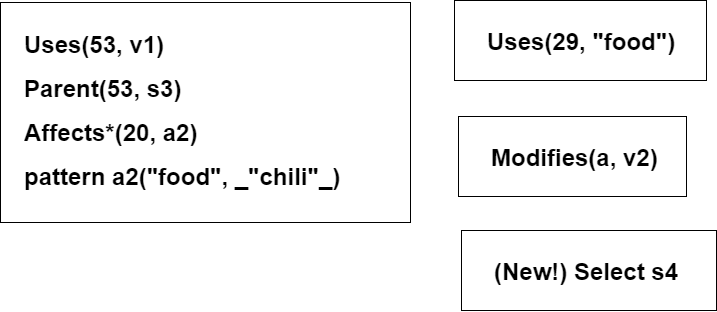
\includegraphics[width=0.7\textwidth]{Optimizer1}
\end{minipage}
\end{center}
\item Sort clauses within each clause groups based on their costs, then chain them up such that clauses with two synonyms have one of the synonyms evaluated before it is evaluated (unless all clauses in the group has two synonyms).
\item Sort clause groups based on the total cost of clauses in each clause group.
\begin{center}
\begin{minipage}{\linewidth}
\centering
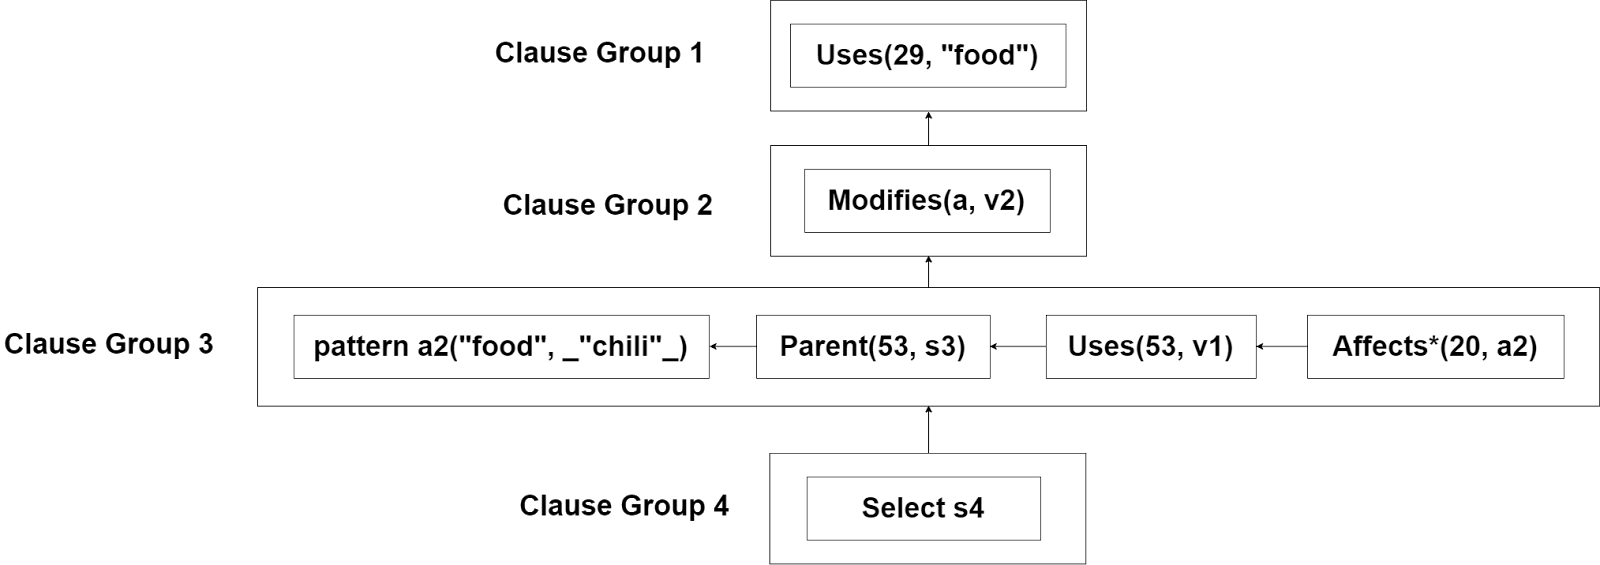
\includegraphics[width=1.0\textwidth]{Optimizer2}
\end{minipage}
\end{center}
\item Pass the queue of ClauseGroup created to ClauseGroupManager, and pass ClauseGroupManager to the QueryEvaluator.

\end{enumerate}
\subsubsection{Query Evaluator}
The QueryEvaluator is used to retrieve design entities from the PKB that fulfill query specifications. It first retrieves the Clause objects (created by the QueryValidator) from the QueryTree. For each Clause object, the QueryEvaluator will evaluate the clause with the help of appropriate ClauseEvaluators and proceed with the evaluation. These evaluators assist the QueryEvaluator in retrieving the relevant results from the PKB and are produced by providing Clause object to the ResultFactory.
\begin{figure}[H]
  \centering 
  \caption{ClauseResult}
 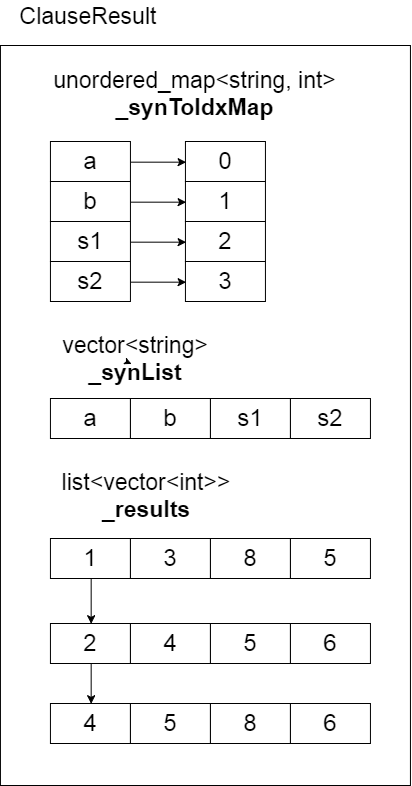
\includegraphics[width=0.3\textwidth]{ClauseResult.png}
\end{figure}

The ClauseResult is responsible for storing and maintaining the intermediate results across Clause objects as they are evaluated by the QueryEvaluator. The ClauseResult maintains several data structures to achieve this purpose.

The intermediate results are stored in a list<vector<int> > data structure, where each vector<int> represents one combination of all synonyms that satisfy the clauses evaluated so far. A vector is used to store these combinations because it allows access of the values of selected synonyms in $O(1)$ time with indexing. This means that every index position in the vector is mapped to a certain synonym, and this mapping is the same for all vectors in the list. A list is used to store these vectors because combinations of synonym values (rows) will need to be inserted and removed from the middle of the list often, and a linked-list can carry out these operations in $O(1)$. As vectors are used for rows, frequent deletion of columns can be inefficient, since the elements after the deleted column will need to be shifted forward. As such, when doing pruning (more in the Optimiser’s section), instead of actually deleting columns, what happens is the column values will be set to -1. When this happens, several previously different rows may now become the same.
\begin{figure}[H]
  \centering 
  \caption{Pruning Synonym “b” in ClauseResult}
 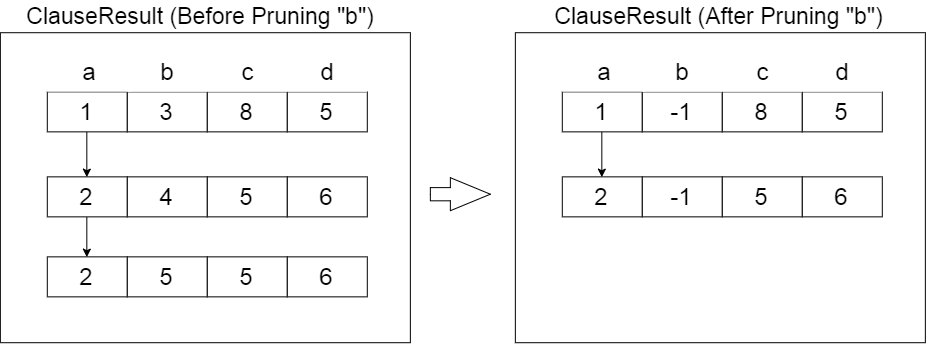
\includegraphics[width=0.7\textwidth]{Pruning.png}
\end{figure}
Duplicates can then be removed and the size of the ClauseResult will be reduced.\newline
As the index positions in the aforementioned vectors need to be mapped to synonyms, an unordered\_map<string, int> is used to store the mapping between synonyms and their indices, and a list<string> is used to implicitly store the reverse mapping.


\textbf{Evaluation Process} \newline
The evaluation steps are listed below:

As per the \textbf{Strategy} pattern, each clause in the clause group will have an evaluator created specially for its evaluation. Figures 16,17 and 18 show an overview of the various evaluators, derived from the base class ResultEvaluator. 
\begin{enumerate}
\item When invoked, the evaluate method of the QueryEvaluator will first initialise the QueryOptimiser, which will split the ClauseObjects based on common synonyms and put them into ClauseGroups. ClauseObjects within each ClauseGroups are then sorted based on the estimated cost and ClauseGroups are also sorted based on the total cost of all the ClauseObjects in them.
\item The sorted ClauseGroups are then passed to the ClauseGroupManager, which is then returned to the QueryEvaluator. The QueryEvaluator can obtain the ClauseGroups, one after the other, from the ClauseGroupManager. The Clause objects will be processed in the groupings and order that the QueryOptimiser has determined.

\item The QueryEvaluator then initialises the ResultFactory and feeds the Clause objects, one at a time, to the ResultFactory that needs to be processed. The ResultFactory will iterate through all the ClauseGroups given by the ClauseGroupManager. Each ClauseGroup will produce a ClauseResult. At any point, if one clause should return false due to invalid evaluation or all results get removed from the ClauseResult, the whole evaluation process will be discontinued, even if it is from another ClauseGroup.

\item As per Strategy pattern, the ResultFactory will create evaluators specially for the evaluation of the clauses. Figures 17,18 and 19 show the overview of the various evaluators that can be created.
   \begin{center}
\begin{figure}[H]
  \caption{With Evaluator}
 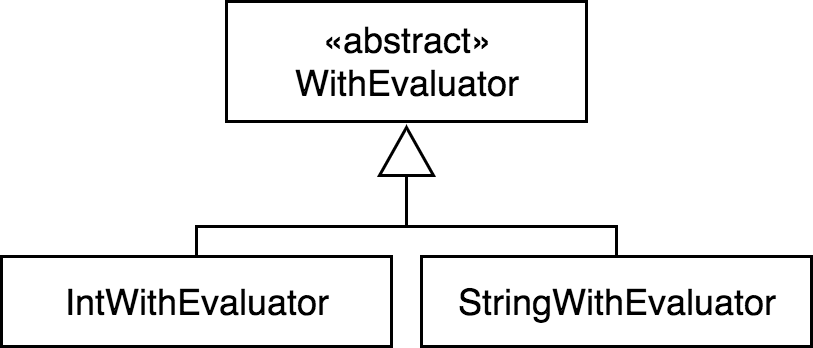
\includegraphics[width=0.5\textwidth]{WithEvaluator.png}
\end{figure}
\end{center}
\begin{figure}[H]
  \centering 
  \caption{Pattern Evaluator}
 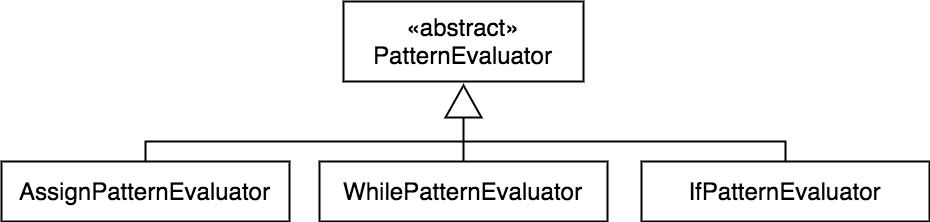
\includegraphics[width=0.8\textwidth]{PatternEvaluator.png}
\end{figure}
\begin{figure}[H]
  \centering 
  \caption{Such That Evaluator}
 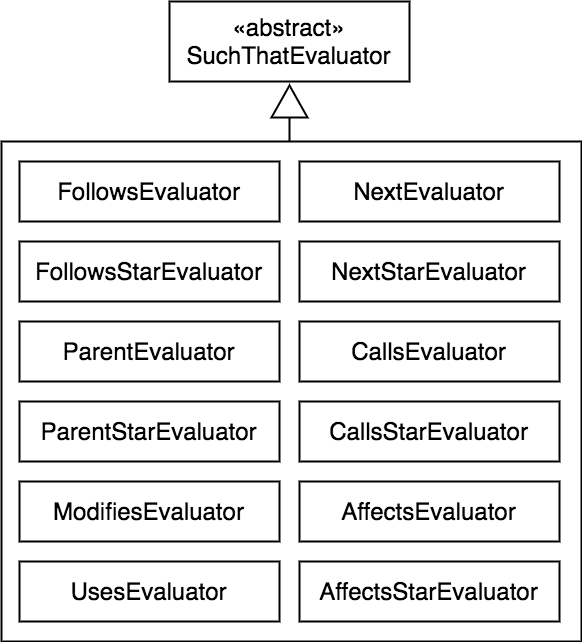
\includegraphics[width=0.5\textwidth]{SuchThatEvaluator.png}
\end{figure}
Generation of an evaluator is done via the Factory pattern, using the information retrieved from Clause objects. The appropriate evaluator is chosen based on the type reference of the Clause objects. For example, the SuchThatEvaluator has a relationship type specifier while the PatternEvaluator has a pattern type specifier.
\item Evaluators determine how to evaluate results by passing the arguments of a clause through several cases. Each clause will have its own case to evaluate depending on the type of inputs that they allow. Table 4 shows an example of the evaluation cases for the Follows relationship.
\begin{table}[H]
  \centering 
  \caption{Follows Evaluator Cases}
 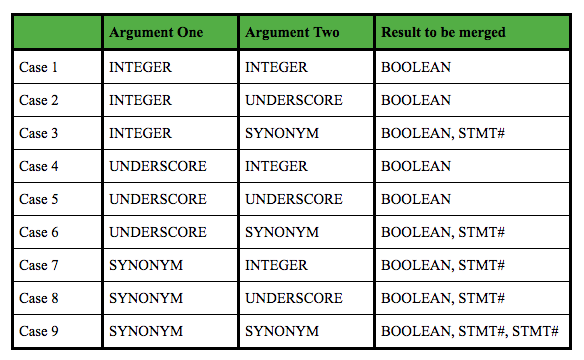
\includegraphics[width=0.6\textwidth]{FollowsEvaluatorCases.png}
\end{table}
\item After the specific evaluators evaluate the clauses, the results of the current clause will be merged into the ClauseResult object, which keeps track of the intermediate results of the ClauseGroup that the evaluator is currently evaluating. For purely Boolean cases (i.e. Follows(3, 4); Case 1 in Table 4), only the validity is returned by the evaluator, and this determines whether evaluation will proceed with the next clause. The validity replaces any previously stored boolean value. Recall that the evaluating process will be terminated if the stored validity is false; thus a false stored validity will never be overwritten . For cases with Synonyms , the validity is returned, and results are stored or modified in the ClauseResult via its reference pointer.
\item For clauses that contain synonyms, there are 5 possible cases that may arise.
\begin{table}[H]
  \centering 
  \caption{Cases of Clauses with Synonyms}
 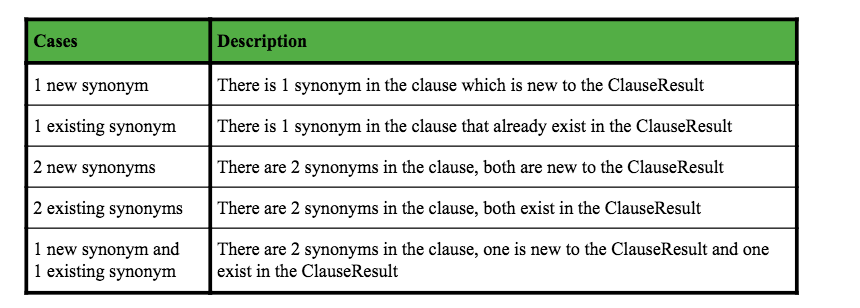
\includegraphics[width=1.0\textwidth]{SynonymClauses.png}
\end{table}
For the cases of 1 new synonym and 2 new synonyms, the way the ClauseResult works depends on whether there are already other synonyms existing in the ClauseResult. These two scenarios are illustrated in the following diagram.
\begin{figure}[H]
  \centering 
  \caption{Adding New Single Synonym Results}
 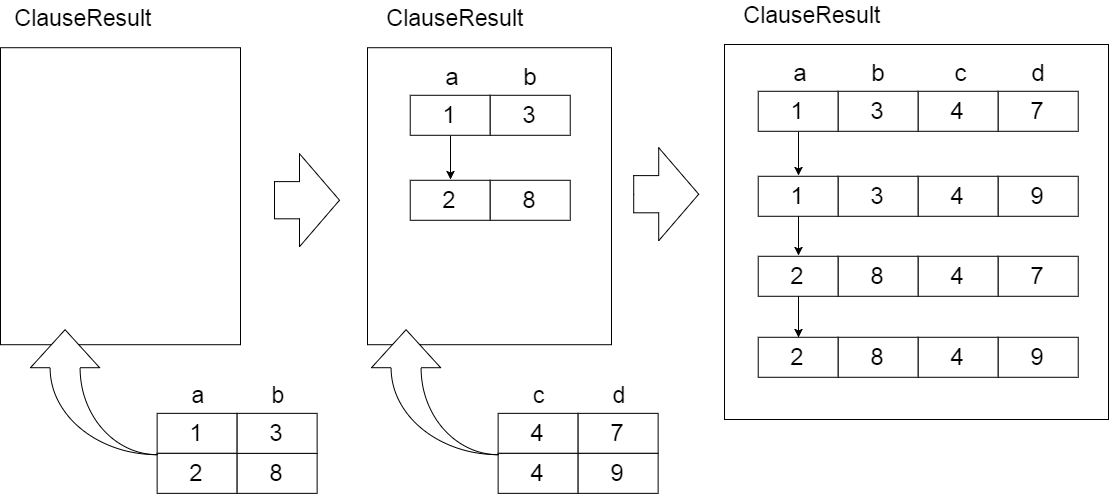
\includegraphics[width=0.8\textwidth]{ClauseResult_AddTwoNew.png}
\end{figure}
Notice that for the case of 2 new synonyms, PKB will need to compute all pairs of the two synonyms for evaluator, which is an expensive process. Optimisation to avoid this scenario is possible, which will be introduced in future iterations. \newline For the cases of 1 existing synonym and 2 existing synonyms, the ClauseResult will loop through the existing results and remove the ones that do not have a match in the new result list
\begin{figure}[H]
  \centering 
  \caption{Adding Existing Synonym Results}
 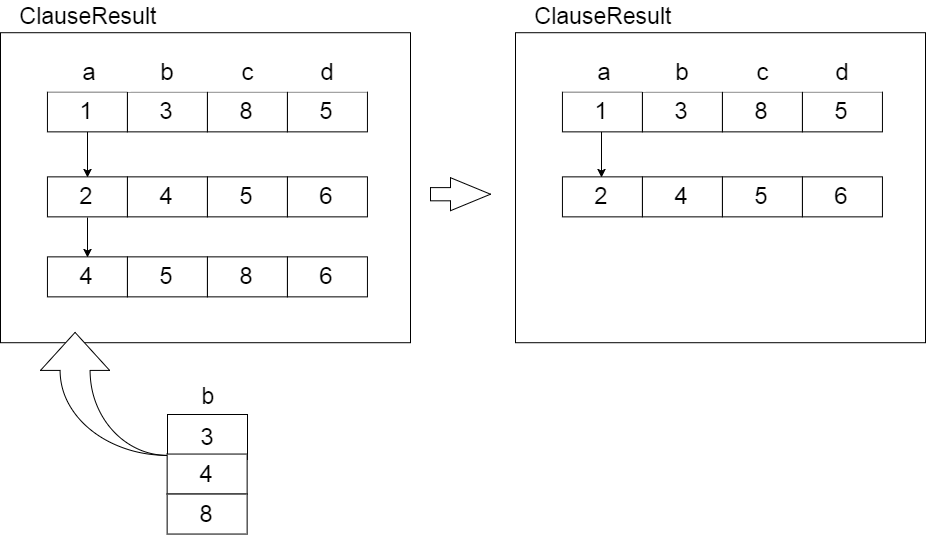
\includegraphics[width=0.8\textwidth]{ClauseResult_AddExistingSynonym.png}
\end{figure}
\begin{figure}[H]
  \centering 
  \caption{Adding A New Synonym Paired to an Existing Synonym}
 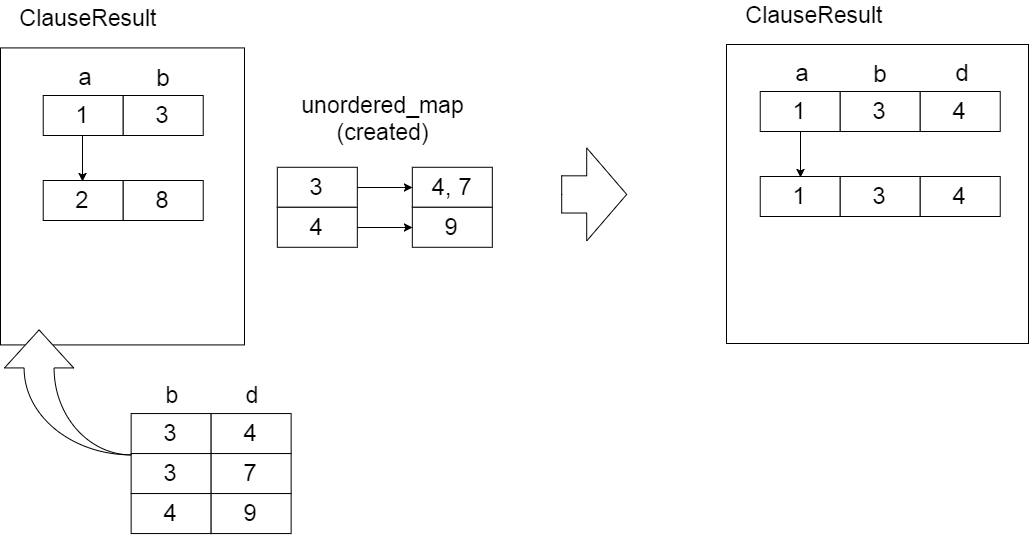
\includegraphics[width=0.8\textwidth]{ClauseResult_AddOneNewOneExisting.png}
\end{figure}
For the case of 1 new synonym and 1 existing synonym, the ClauseResult will do the merging of result using \textit{hash join}. An unordered\_map<int, list<int> > will be created to help with the merging process, this unordered\_map will map each values of the existing synonyms to the list of the corresponding values of the corresponding new synonym. For each of the existing result combination, if the common synonym’s value has a match in the unordered\_map, the new synonym’s value will be appended to the combination. If the common synonym’s value has no match in the unordered\_map, the combination will be discarded.

If the number of combinations of the existing results is $M$, and that of the results to merge is $M$, the time complexity of this merging process would be $O(M+N)$, which is sufficiently fast.

\item Each ClauseGroup will yield one ClauseResult object. After the ResultFactory has finished processing all the Clause objects in a ClauseGroup, and all of them return true for validity, the factory will pass the evaluated ClauseResult to the ClauseGroupManager. The ClauseGroupManager maintains an internal ClauseResult that only contains all the selected synonyms’ result from all ClauseGroups. When the ClauseGroupManager receives a newly evaluated ClauseResult from the QueryEvaluator, it will sieve the results of the selected synonyms and merge them into the internal ClauseResult. After all ClauseGroups has been processed, the ClauseGroupManager will return the final merged ClauseResult of all ClauseGroups  to the QueryEvaluator and QueryEvaluator will then store this back into the QueryTree, waiting for it to be picked up by the ResultFormatter to format and return the final result.

\end{enumerate}
\subsubsection{Result Formatter}
The ResultFormatter uses the QueryTree and the ClauseResult to return results in the form of a list of strings (list<string>)  back to the UI. It first checks the type of the Select clause (whether it’s BOOLEAN, single synonym or tuple). 
\begin{enumerate}
\item If the query selects BOOLEAN, the ResultFormatter checks whether the ClauseResult has results and if QueryTree has any clauses to evaluate. If QueryTree contains clauses to evaluate, if ClauseResult doesn’t have results after evaluation, then the ResultFormatter returns a ‘false’ result; it returns ‘true’ for all other cases.
\item If the query selects a single synonym/tuple, then ResultFormatter uses ClauseResult’s API getSynonymResults() to get the raw results. If the synonym being selected returns a numerical result, then the list of integers (list<int>) is converted to a list of strings (list<string>) and projected to the UI. 
In case the synonym being selected needs to return a string result (e.g entities of the type VARIABLE,PROCEDURE or CALL.PROCNAME) the list of integers received from ClauseResult are converted to a list of strings according to the mapping done by PKB (as previously, we map all strings to ints to optimize Query Evaluator; thus, we need to convert the mapped ints to strings when we output the results)
\end{enumerate}
\subsection{Design decisions}
\subsubsection{Parsing Strategy}
\begin{tabular}{|L{5cm} | L{12cm}| }
\hline
Problem &
The Parser has a lot to do while parsing the SIMPLE source code:\newline
- Various types of syntax validation
\newline - Display error message as user feedback when syntax error is detected
\newline - Extract various design abstractions and populate PKB
 \\
    \hline
    Alternatives &
1. Do all of the job of the parser in one parse
\newline 2. Do many parses, each parse doing one particular task, e.g. bracket-matching, Calls relation, Uses relation, etc.
\newline 3. Hybrid of the above two alternatives. \\
\hline
    Criteria for comparison &
1. Time-efficiency
\newline 2. Ease of implementation
\newline 3. Testability
\newline 4. Maintainability
\newline 5. Extensibility to future iterations, and possible bonus features 
 \\
 \hline
   Decision & \textbf{Choice: Hybrid}
\newline
Doing everything in one parse can be difficult to implement and error-prone. It also makes testing difficult. On the other extreme, having many parses, each doing one simple task, will also result in a lot of duplicate codes, which will make parser difficult to maintain and extend.
\newline
Therefore, using just a few parses with each parse doing related tasks is the most reasonable design. The Parser will do one parse just to check whether braces are paired up correctly, and do a second parse to extract design abstractions and populate PKB.
 \\
 \hline
\end{tabular}
\subsubsection{PKB Design: Representation of Design Abstraction}
\begin{tabular}{|L{5cm} | L{12cm}| }
\hline
Problem &
Speed is a very important aspect for query evaluation. If this aspect is neglected, it would cause a longer runtime when multiple queries are processed. Therefore, design of the data structures to store and represent design abstractions is extremely crucial to ensure that data is accessible in the shortest time possible.
 \\
    \hline
    Alternatives &
- AST
\newline - Tables in the form of: \begin{itemize}
\item Hash maps
\item Vector of lists
\end{itemize} 
 \\
\hline
    Criteria for comparison &
1. Time complexity of retrieval, addition and deletion
\newline 2. Simplicity of implementation 
\newline 3. Extensibility to future iterations and possible bonus features
\newline 4. Testability
 \\
 \hline
   Decision & \textbf{Choice: Tables in the form of hash maps}
\newline
Abstract Syntax Tables are the conventional ways to store parsed data. However, when it comes to accessing the data by the Query Evaluator component, it will have to perform traversing of the tree, which could take a lot of time during Query Processing. Also, doing modifications to allow more design entities would be more complicated. Alternatively, hash maps can be used to store data. Having multiple hashmaps rather than an AST allows faster searching, addition, deletion of data. 
\newline Data structures used in the implementation of tables include:
\newline 1. Vectors of lists of strings/integers
\newline 2. Hashmap with integer as hash key and list of string/integers as value \newline
Amongst the two data structures listed above, hash maps are preferred over vectors due to their fast lookup speeds. To find the desired data in a vector, linear traversal is needed to get to its relative index at a time complexity of $O(n)$, which turns out to be slower than AST, that takes $O(log n)$ time. On top of this, unlike hash maps, vectors does not take strings as index for data mapping. Having multiple hashmaps over ASTs allow faster searching, addition and deletion of data.

 \\
 \hline
\end{tabular}
\newline The table below shows the time complexity of query processing when AST and tables are used. '$s$' represents the number of statements in the SIMPLE programme):
\begin{table}[htbp]
\begin{tabular}{|c|c|c|c|}
\hline
 & Using AST & Hash Maps & Vectors\\
\hline
Data searching & $O(log\hspace{1mm}s)$ & $O(1)$ & $O(s)$\\
\hline
Retrieving single data & $O(log\hspace{1mm}s)$& $O(1)$ & $O(s)$\\
\hline
Retrieving all the data & $O(s\hspace{1mm}log\hspace{1mm}s)$ & $O(s)$ & $O(s)$\\
\hline
\end{tabular}
\end{table}
\subsubsection{PKB Design: Evaluating reverse relationships}
\begin{tabular}{|L{5cm} | L{12cm}| }
\hline
Problem &
For queries that require retrieval of the left hand parameter (as in x in Uses(x,y), Modifies(x,y), etc.), the key of the hash map needs to be retrieved from the input value. For example, if the Query Evaluator calls Follows(3, s), statement s can be retrieved in $O(1)$ time, by using the key ‘3’. However, if Follows(s, 3) is called, since ‘s’ is an unknown key, it is not possible to retrieved in constant time. Therefore, traversing is needed to find the key that matches with the value, and it could take $O(n)$ time complexity at its worst.
 \\
    \hline
    Alternatives &
- Add another hash maps to store reverse relationships
\newline - Self-balancing binary search tree (BST) 
 \\
\hline
    Criteria for comparison &
1. Time complexity for retrieval
\newline 2. Ease of implementation
 \\
 \hline
   Decision & \textbf{Choice: Add another data structure to store reverse relationships}
\newline
The time complexity of searching in hash maps is faster compared to searching in trees, as traversing of trees takes $O(log n)$ time. A drawback in this method is that adding an extra data structure doubles the space complexity, but the priority of this SPA is the speed and efficiency of data retrieval, rather than the size of the program. Therefore, sacrificing memory space for better speed is more practical.
 \\
 \hline
\end{tabular}
\subsubsection{PKB Design: CFG Design}
\begin{tabular}{|L{5cm} | L{12cm}| }
\hline
Problem &
Storage of CFG
 \\
    \hline
    Alternatives &
- Adjacency List
\newline - Adjacency Matrix
\newline - Edge List

 \\
\hline
    Criteria for comparison &
1. Time complexity for finding relation
\newline 2. Time complexity for traversal
\newline 3. Ease of implementation
 \\
 \hline
   Decision & \textbf{Choice: Adjacency List}
\newline
Time complexity for finding relation: Edge List $O(E)$ > Adjacency List $O(2)$ = $O(1)$ = Adjacency Matrix $O(1)$. \newline
Time complexity for traversal: Edge List $O(E)$ > Adjacency Matrix $O(V^2)$ > Adjacency List $O(V)$ \newline
Time complexity for finding relation in Adjacency List in our CFG is $O(1)$ as each statement in the CFG can have at most 2 vertices. Therefore, Adjacency List is the best for retrieval of a relation as well as for graph traversal. At the same time, the way PKB stores next relations are already in an Adjacency List format. Hence it is easier to use the table of all next statements as our Adjacency List.

 \\
 \hline
\end{tabular}
\subsubsection{Pattern Matching: Representation of expressions}
\begin{tabular}{|L{5cm} | L{12cm}| }
\hline
Problem &
Pattern matching requires consideration of the precedence of operators and associativity, therefore it cannot be performed by matching substrings. Therefore, an alternate representation of expressions is required to facilitate pattern matching.
 \\
    \hline
    Alternatives &
- Trees to represent expression
\newline - Postfix matching


 \\
\hline
    Criteria for comparison &
1. Time complexity of retrieval
\newline 2. Simplicity of implementation
\newline 3. Testability
 \\
 \hline
   Decision & \textbf{Choice:  Postfix matching}
\newline
Postfix matching is used instead of trees due to the fact that trees are harder to implement and make debugging more time consuming. Postfix expressions can be represented in a list of strings containing operator/operands, and they can be easily inserted into and retrieved from hash maps. Pattern matching can be done by comparing sublists.
 \\
 \hline
\end{tabular}

\subsubsection{Affects* Computation Decision
}
\begin{tabular}{|L{5cm} | L{12cm}| }
\hline
Problem &
Computation of any Affects* relation
 \\
    \hline
    Alternatives &
- Running Affects* algorithm for each query
\newline - Computing all Affects* relations and storing it in the cache and then retrieving the required relations


 \\
\hline
    Criteria for comparison &
1. Time-efficiency
\newline 2. Memory required
 \\
 \hline
   Decision & \textbf{Choice:  Computing all Affect* relations and storing it in the cache then retrieving the required relations}
\newline
Shorter computation time for future Affects* clauses.
\newline
As the algorithm for get the boolean result of an Affects* relation such as Affects*(3, 10), it requires the computation of the transitive closure of all Affects relations and checking if it exists. Since the computation time for all Affects relations is about the same as computing all Affects* relations as they are both a one-pass algorithm, it is much faster to compute all Affects* relations and then getting the required relations in $O(1)$ from the cache. Another benefit of doing this is that all the following Affects* relations following the first Affects* clause in the query could be retrieved from the PKB in $O(1)$. For example, Affects*(1, 3) and Affects*(a, 100) and Affects*(a1, a2), the relations can all be retrieved in $O(1)$ following the first Affects*(1, 3) call.

 \\
 \hline
\end{tabular}



\subsubsection{Affects* Design Decision
}
\begin{tabular}{|L{5cm} | L{12cm}| }
\hline
Problem &
Extraction of all Affects* pairs 	
 \\
    \hline
    Alternatives &
- Brute force
\newline - One-pass


 \\
\hline
    Criteria for comparison &
1. Time-efficiency
\newline 2. Readability of code
 \\
 \hline
   Decision & \textbf{Choice:  One-pass}
\newline
Shorter computation time.

As Affects* can only be computed on the run during the evaluation of a query, it is very time consuming to run the Affects* algorithm on every assignment statement as it requires the traversal of the CFG $n$ times where $n$ is the number of assignment statements. On top of that, it requires additional time for extra checking of uses and modifies variables in each assignment statement.


 \\
 \hline
\end{tabular}


\subsubsection{Query Validation Design}
\begin{tabular}{|L{5cm} | L{12cm}| }
\hline
Problem &
1. Difficulty in parsing query
\newline 2. Too many if-else string comparisons
 \\
    \hline
    Alternatives &
1. Usage of Regular Expression
\newline 2. Naive tokenizing with specific delimiter
\newline 3. Naive if-else
 \\
\hline
    Criteria for comparison &
1. Time-efficiency
\newline 2. Ease of implementation
\newline 3. Testability
\newline 4. Maintainability
\newline 5. Extensibility to future iterations and possible bonus features\\
 \hline
   Decision & \textbf{Choice:  Regular Expression}
\newline
Parsing the query may be tedious as there are many considerations to take into account to when choosing the delimiters. Regex provides a fast and elegant solution. One line of regex can replace a hundred lines of procedural code. As members of  the group are well-versed and experienced with regex, implementation was fast. Regex is easier to maintain, especially when they are stored in string constants that can be reused and concatenated to form a larger expression.
 \\
 \hline
\end{tabular}
\newline
\begin{tabular}{|L{5cm} | L{12cm}| }
\hline
Problem &
Many “if-else” statements to handle the validation of clauses
 \\
    \hline
Alternatives &
Strategy pattern (Handlers and sub-validators)
 \\
\hline
Criteria for comparison & 
1. Ease of implementation \newline 2. Ease of extension \newline 3. Testability \newline 4. Memory overhead
 \\
\hline
Decision &
Choice : Strategy Pattern \newline

\textbf{Justification} \newline
1. Easy modification and extension as understanding the individual strategy to process each clause does not require you to understand the entire process.
\newline 2. Less tedious to maintain and extend the code as changes only need to be done in a class design as compared to all classes.
\newline 3. Eliminates conditional statements for selecting the correct validator to process each clause. 
\\
 \hline
\end{tabular}
\subsubsection{Query Evaluation Design}
\begin{tabular}{|L{5cm} | L{12cm}| }
\hline
Problem &
Many “if-else” statements to handle the evaluation cases of all the clauses, deeply nested nested if else blocks makes extension of the evaluators very tedious
 \\
    \hline
Alternatives &
1. Strategy pattern (ClauseEvaluator and sub-classes)
\newline 2. Factory pattern (ResultFactory and ClauseResult)
 \\
\hline
Criteria for comparison & 
1. Ease of implementation \newline 2. Ease of extension \newline 3. Testability \newline 4. Memory overhead
 \\
\hline
Decision &
\textbf{Justification: Strategy Pattern} \newline
1. Modifying or understanding the individual strategy to process each clause does not require you to understand the entire process.
\newline 2. Less tedious to maintain and extend the code as changes only need to be done in a class design as compared to all classes.
\newline 3. Eliminates many conditional statements for evaluator to select the correct function to process each clause. \newline
\textbf{Justification: Factory Pattern} \newline
1. Lazy initialization to delay creation of the subunit processors to process each clause. 
\newline 2. A single point of control to create the subunit processor, which are evaluators.
\\
 \hline
\end{tabular}

\subsubsection{Data Structure for Intermediate Result}
\begin{tabular}{|L{5cm} | L{12cm}| }
\hline
Problem &
The data structures of intermediate result is crucial for the good performance of PQL queries as numerous operations will need to be carried out on the intermediate result when evaluating each clause. These operations include merging of tables, insertions, deletions, and many more, which might be computationally expensive if not optimised.
 \\
    \hline
    Alternatives & Representation of results: \begin{enumerate}
    \item Vector of vectors
    \item List of vectors
    \end{enumerate} \\
\hline
    Criteria for comparison &
Time-efficiency is the major criteria, as the process of merging intermediate results is one of the most expensive and most carried-out operation in the query evaluation process. \\
 \hline
   Decision & \textbf{Choice of data structure: Linked-list of vectors}
\newline
Each vector represents a possible combination of synonym values that satisfy a query, with each index assigned to a particular synonym for $O(1)$ access.

Using a linked-list to chain up all the possible combination of synonyms will allow very fast insertion and deletion of existing combination of synonym results in the middle of the list. Insertion/deletion takes $O(1)$. This will enhance performance tremendously,compared to using a vector of vectors.
 \\
 \hline
\end{tabular}

\subsubsection{Query Optimiser - Cost Allocation for Clauses}
\begin{tabular}{|L{5cm} | L{12cm}| }
\hline
Problem &
How to assign cost to clauses in query
 \\
    \hline
    Alternatives & \begin{enumerate} \item Static cost allocation based on statistics and general heuristics \item Dynamic cost allocation based on information in PKB
\item Hybrid of static and dynamic cost allocation \end{enumerate}

 \\
\hline
    Criteria for comparison &
\begin{enumerate} \item Time-efficiency \item Ease of implementation
\item Optimization overhead \end{enumerate}
 \\
 \hline
   Decision & \textbf{Choice: Static cost allocation based on statistics and general heuristics}
   \newline Justification
\begin{enumerate}
\item The time-efficiency achieved using dynamic cost-allocation is, most of the time, similar to that of static allocation.
\item Ease of implementation
\item Sufficiently efficient for the intended application. Reduce optimisation overhead
\end{enumerate}
 \\
 \hline
\end{tabular}
\section{Documentation and Coding standards}
We follow a combination of Coding Standards from different sources in order to get an optimal set of rules that help us the most in our project.
\subsection{Abstract API and Concrete API}
We made our Abtract API as similar as we could to concrete APIs in C++ to avoid confusion. At the same time, we tried to keep our Abstract API programming language independent and made it general enough to be implementable. Ex. Abstract API LISTSTMT was implemented with a concrete API of list<string>.
\subsection{Naming Conventions}
We follow the naming conventions detailed in this website 
\href{http://geosoft.no/development/cppstyle.html#Naming Conventions}{\textbf{Geosoft C++ naming conventions}}
\begin{itemize}
\item Method names should clearly describe their intended functions. 
\item Camel cases are used for naming of methods, parameters and variable.
(E.g addWhileStmt(int stmt, string controlVar), varIdx, etc)
\item Pascal cases are used for naming of classes and files. (E.g FollowsTable, UsesTableStmtToVar)
\item Prefixes that start with ‘\_’ are named in private methods.
(E.g \_pkbMainPtr, \_isValidSyntax)
\item Uppercase is used for naming of constants, separated by ‘\_’ for each word.
For example: REGEX\_VALID\_ENTITY\_NAME, INT\_INITIAL\_PROC\_INDEX
\item To represent star relationships, ‘Star’ is used in naming of classes, methods and files. For example Follows* is represented as FollowsStar.
\end{itemize}
\subsubsection{Formatting}
We follow the formatting detailed in this website 
\href{https://google.github.io/styleguide/cppguide.html#Formatting}{\textbf{Google style C++ formatting}} 
\newline Some standard rules we follow are given below.
\begin{itemize}
\item We use 4 whitespaces as our default indentation.
\item Every class must contain one .h file and one .cpp file, and the class, .h files and .cpp files must have the same name.
\item For use for braces in methods or container statements, we have opening braces and closing braces both on a new line.
\end{itemize}
\subsection{Class hierarchy}
We store our SPA components in separate directories, divided into Parser, PKB and PQL. Our design abstractions are stored in separate source files (.cpp) and our concrete APIs are defined in the corresponding header files (.h).


\section{Testing}
Our testing objectives are: 
\begin{enumerate}
\item To discover possible defects and loopholes which may arise while developing the SPA
\item To gain confidence in developing and maintaining the  SPA
\item To ensure the final product meets the SPA requirements
\end{enumerate}
\subsection{Test Plan}
The testing process consists of 3 stages, namely Unit Testing, Integration Testing and System Testing. For every new functionality added or modification made to the SPA, these tests are rerun. This ensures that newly added function produces the expected result. Regression testing is conducted to ensure that the changes do not affect previously tested functionalities. With all these tests put in place, the code remains buildable at all times. If there were any bugs, it can be resolved promptly.
\begin{figure}[h]
  \centering 
  \caption{Flow chart showing the testing process}
 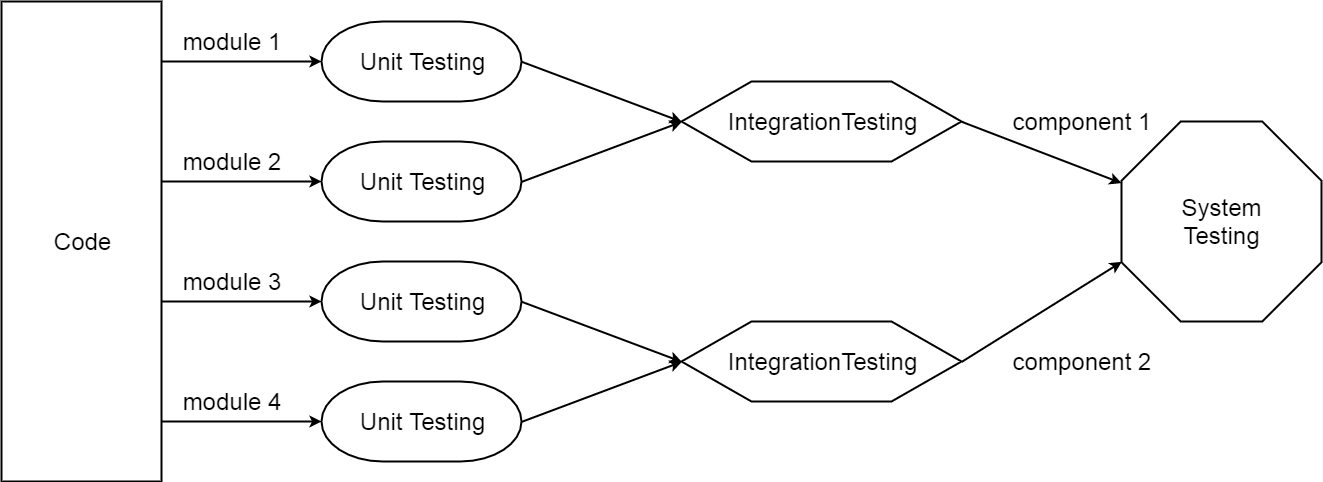
\includegraphics[width=0.8\textwidth]{Testing_process.png}
\end{figure}
Do refer to Section 5.5 for further details on our System Testing.
\subsubsection{Test Schedule for All Iterations}
For each iteration, unit testing will be conducted during the first half of the iteration, to ensure that the new modules introduced produced the expected result. Algorithms are verified and logical errors will be corrected during this process. Private methods are tested by creating friend classes and accessing them using the these friend classes. Individual developers are responsible for testing their own code. Integrating testing will be conducted to ensure that these modules are able to communicate and interact with other components as expected. For example, tests are written to check whether QueryValidator is able to store data into the QueryTree, and whether the retrieved data from QueryTree are the same as those stored by the QueryValidator. Towards the end of each iteration, system testings are carried out frequently using the AutoTester to check for regression. Two developers are delegated to creating new source programs and generating queries that covers corner cases. At any point during the testing process, bugs that surface will be resolved immediately by the developer of the component.
\begin{figure}[h]
  \centering 
 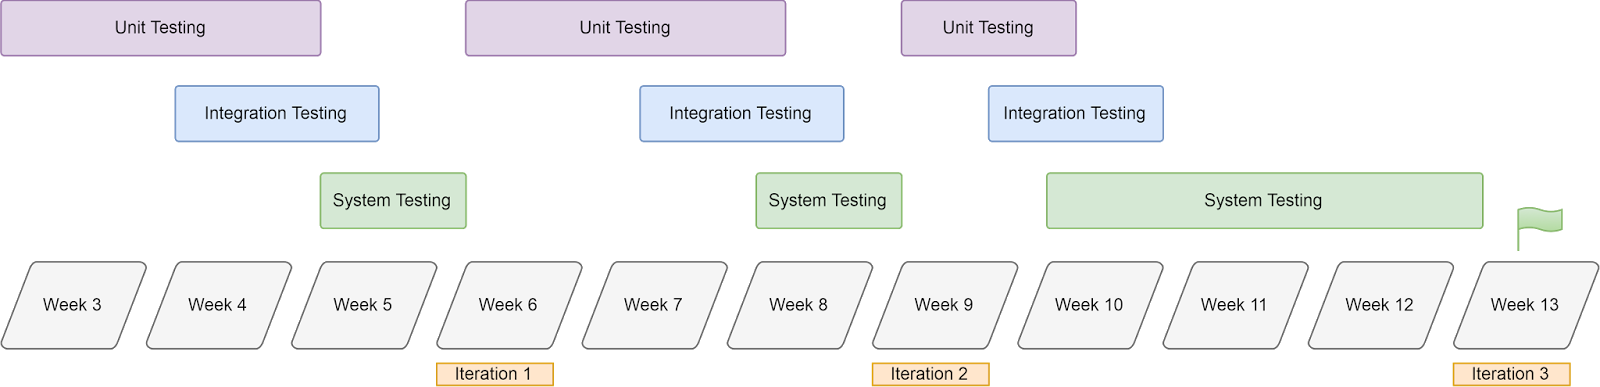
\includegraphics[width=1.0\textwidth]{test_schedule.png}
\end{figure}

\subsubsection{Test Objectives}
We use 3 different types of procedures to detect bugs within our SPA.
\begin{enumerate}
\item Unit testing (white-box testing)
\item Integration testing
\item System testing
\end{enumerate}
\newpage
The following components are subjected to testing: \newline
\small
\begin{tabular}{|L{3cm} | L{13cm}| } 
\hline
\textbf{Component} &
\textbf{Objectives}
 \\
    \hline
    Parser &
\begin{itemize}[noitemsep]
\item To ensure that the source file is parsed and validated accurately
\item To ensure that the correct information is stored into PKB
\end{itemize}  \\\hline
    Design Extractor &
\begin{itemize}[noitemsep]
\item To ensure that the computation of transitive closure and computation of star relationships are done correctly
\end{itemize}  \\\hline
 PKB &
\begin{itemize}[noitemsep]
\item To ensure that information can be stored successfully
\item To ensure that the information retrieved from PKB is accurate and expected
\end{itemize}  \\\hline
 Query Validator &
\begin{itemize}[noitemsep]
\item To ensure that the query is parsed and validated accurately
\item To ensure that the query is partitioned accurately
\item To ensure that the partitions are stored in the QueryTree accurately
\end{itemize}  \\\hline
 Query Evaluator &
\begin{itemize}[noitemsep]
\item To ensure that the information retrieved from the QueryTree is accurate
\item To ensure that the result retrieved from the PKB is accurate
\item To ensure that merged result of various clauses produce the expected result
\end{itemize}  \\\hline
 Query Tree &
\begin{itemize}[noitemsep]
\item To ensure that the information is stored successfully
\item To ensure that the information is retrieved correctly
\end{itemize}  \\\hline
\end{tabular}

\normalsize
\subsection{Test Utilities Class}
Test utilities classes provide helper methods to aid the unit testing and integration testing process.

\begin{tabular}{|L{5cm} | L{12cm}| }
\hline
\textbf{Class} &
\textbf{Description}
 \\
    \hline
    ParserChild &
A child class of Parser. It access the protected methods and variables and made them available for unit testing. \\\hline
 UtilityQueryTree &
Retrieves information from QueryTree and compare with the data expected to be retrieved. It is mainly used in integration testing of DeclarationValidator and QueryTree.  \\\hline
UtilitySelection &
Makes the different clause objects that contain expected data. It is mainly used in the integration testing of QueryValidator and ResultFormatter.  \\\hline
 FriendDeclarationValidator &
Friend class of DeclarationValidator. It access the private methods and variables and made them available for integration testing.  \\\hline
\end{tabular}


\subsection{Unit Tests}
Unit testing involves the testing of individual modules within the component, as well as the component itself, isolated from other components of the system. It is a form of white-box testing, where test cases specifically targets the internal structure of the module.

\subsubsection{PKB Unit Test}
Before the start of the test, pre-defined relationships are injected directly into the PKB table.


\begin{longtable}{|L{5cm} | L{12cm}| }
\hline
\textbf{Test Purpose} &
To test if PKB computes design entity, stmt,  correctly
\\\hline
\textbf{Required Test Input}
 &
 \texttt{
 \noindent TEST\_METHOD(TestGetStmt)
\newline \vspace{2mm}
 \{ \hspace{4mm} FollowsTable table; \newline \vspace{2mm}
 \hspace{9mm} Assert::IsTrue(table.addFollows(2, 1, 3)); \newline 
 \hspace{9mm} Assert::IsTrue(table.addFollows(3, 2, 4));\newline 
 \hspace{9mm} Assert::AreEqual(table.getStmtAft(2), 3);\newline 
 \hspace{9mm} Assert::AreEqual(table.getStmtBef(2), 1);\newline 
 \hspace{9mm} Assert::AreEqual(table.getStmtAft(3), 4);\newline 
 \hspace{9mm} Assert::AreEqual(table.getStmtBef(3), 2); \} }

 \\\hline
   \textbf{ Expected Test Results} &
true, true, true, true, true, true \\\hline
\end{longtable}

\newpage
\begin{longtable}{|L{5cm} | L{12cm}| }
\hline
\textbf{Test Purpose} & To test if PKB computes relation Calls* correctly\\\hline
\textbf{Required Test Input}
 & \texttt{\noindent TEST\_METHOD(TestCallsTable)
\newline
 \{ \hspace{4mm} PKBMain PKB; \newline \vspace{2mm}
 \hspace{9mm} PKB.addVariable("a"); \newline 
    \hspace{9mm} PKB.addVariable("b"); \newline 
	\hspace{9mm} PKB.addVariable("c"); \newline
	\hspace{9mm} PKB.addVariable("d"); \newline
	\hspace{9mm} PKB.addVariable("e"); \newline
	\hspace{9mm} PKB.addVariable("f"); \newline
	\hspace{9mm} PKB.addVariable("g"); \newline
	\hspace{9mm} PKB.addVariable("h"); \newline
	\hspace{9mm} PKB.addVariable("i"); \newline
	\hspace{9mm} PKB.addProcedure("One"); \newline
	\hspace{9mm} PKB.setCallsRel(2, "One", "Two"); \newline
	\hspace{9mm} PKB.setCallsRel(3, "One", "Three"); \newline
	\hspace{9mm} PKB.setUseTableProcToVar("One", "a"); \newline
	\hspace{9mm} PKB.addProcedure("Three"); \newline
	\hspace{9mm} PKB.setCallsRel(6, "Three", "Four"); \newline
	\hspace{9mm} PKB.setCallsRel(7, "Three", "Five"); \newline
	\hspace{9mm} PKB.setCallsRel(8, "Three", "Six");  \newline
    \hspace{9mm} PKB.addProcedure("Four"); \newline
	\hspace{9mm} PKB.addProcedure("Five"); \newline
	\hspace{9mm} PKB.setCallsRel(14, "Five", "Six"); \newline
	\hspace{9mm} PKB.setCallsRel(15, "Five", "Seven"); \newline
	\hspace{9mm} PKB.setUseTableProcToVar("Five", "b"); \newline
	\hspace{9mm} PKB.addProcedure("Six"); \newline
	\hspace{9mm} PKB.setCallsRel(19, "Six", "Seven"); \newline
	\hspace{9mm} PKB.addProcedure("Two"); \newline
	\hspace{9mm} PKB.setCallsRel(24, "Two", "Eight"); \newline
	\hspace{9mm} PKB.addProcedure("Seven"); \newline
	\hspace{9mm} PKB.setCallsRel(28, "Seven", "Nine"); \newline
	\hspace{9mm} PKB.addProcedure("Eight"); \newline
	\hspace{9mm} PKB.setCallsRel(33, "Eight", "Nine"); \newline
	\hspace{9mm} PKB.addProcedure("Nine"); \newline
	\hspace{9mm} PKB.setModTableProcToVar("Two", "b"); \newline
	\hspace{9mm} PKB.setModTableProcToVar("Three", "c"); }
    \\\hline
\textbf{Required Test Input}
 & \texttt{
	\hspace{7mm} PKB.setModTableProcToVar("Four", "d"); \newline
	\hspace{9mm} PKB.setModTableProcToVar("Five", "e"); \newline
	\hspace{9mm} PKB.setModTableProcToVar("Six", "f"); \newline
	\hspace{9mm} PKB.setModTableProcToVar("Seven", "g"); \newline
	\hspace{9mm} PKB.setModTableProcToVar("Eight", "h"); \newline
	\hspace{9mm} PKB.setModTableProcToVar("Nine", "i"); \newline
    \hspace{9mm} list<int> expectedList = { 5, 4, 2, 0 }; \newline
	\hspace{9mm} expectedList.sort(); \newline
	\hspace{9mm} list<int> resultList = PKB.getCallerStar("Seven"); \newline
	\hspace{9mm} resultList.sort(); \newline
	\hspace{9mm} Assert::IsTrue(resultList == expectedList); \newline
	\hspace{9mm} expectedList = { 3, 4, 5, 6, 8 }; \newline
	\hspace{9mm} expectedList.sort(); \newline
	\hspace{9mm} resultList = PKB.getCalleeStar("Three"); \newline
	\hspace{9mm} resultList.sort(); \newline
	\hspace{9mm} Assert::IsTrue(resultList == expectedList); \newline
	\hspace{9mm} pair<list<int>, list<int> > allCallsStar = PKB.getAllCallsStar(); \newline
	\hspace{9mm} Assert::IsTrue(PKB.isCallsStar(0, 2)); \newline
	\hspace{9mm} Assert::IsTrue(PKB.isCallsStar(0, 3)); \newline
	\hspace{9mm} Assert::IsTrue(PKB.isCallsStar(0, 4)); \newline
	\hspace{9mm} Assert::IsTrue(PKB.isCallsStar(0, 5)); \newline
	\hspace{9mm} Assert::IsTrue(PKB.isCallsStar(0, 6)); \newline
	\hspace{9mm} Assert::IsTrue(PKB.isCallsStar(0, 7)); \newline
	\hspace{9mm} Assert::IsTrue(PKB.isCallsStar(0, 8)); \newline
	\hspace{9mm} Assert::IsTrue(PKB.isCallsStar(1, 7)); \newline
	\hspace{9mm} Assert::IsFalse(PKB.isCallsStar(1, 6)); \newline
	\hspace{9mm} Assert::IsFalse(PKB.isCallsStar(1, 4)); \newline
	\hspace{9mm} Assert::IsTrue(PKB.isCallsStar(1, 8)); \} }

 \\\hline
   \textbf{ Expected Test Results} &

true, true, true, true, true, true, true, true, false, false, true
 \\\hline
\end{longtable}

\subsubsection{PQL Unit Test}
In PQL Unit testing, the tests are mostly written to test QueryValidator. In particular, the tests targets the accuracy of the regex of each clause. As QueryValidator determines the argument type by enquiring the QueryTree, semantic checks for the types of arguments are done in the integration tests.

\begin{longtable}{|L{5cm} | L{12.5cm}| }
\hline
\textbf{Test Purpose} &
To test for invalid number of arguments for Follows relationship
\\\hline
\textbf{Required Test Input}
 &
 \texttt{
 \noindent TEST\_METHOD(TestRegex\_Follows\_ArgCount\_inValid)
\newline \vspace{2mm}
\footnotesize \{ \hspace{4mm}  string str = "Follows(validArgsSyntax, with, extraArgs)"; \newline \vspace{2mm}
 \hspace{9mm} Assert::IsFalse(RegexValidators::isValidFollowsRegex(str)); \newline 
 \hspace{9mm}   str = "Follows(insufficientArgs)";\newline 
 \hspace{9mm}  Assert::IsFalse(RegexValidators::isValidFollowsRegex(str));\newline  \} }

 \\\hline
   \textbf{ Expected Test Results} &
false, false\\\hline
\end{longtable}

Another example will be testing of ClauseResult used by the QueryEvaluator. \newline

\begin{longtable}{|L{5cm} | L{12cm}| }
\hline
\textbf{Test Purpose} &
To test the method of ClauseResult (intermediate result) addNewSynPairResults that merges two result tables, namely the existing result and new result, for the case when the clause currently being evaluated is introducing two new synonyms.
\newline \vspace{2mm}
Cases to consider: 
\begin{enumerate}
\item Adding new results when ClauseResult is still empty
\item Adding new results that is a subset of the results that are already in ClauseResult.
\item Adding new results that partially overlaps with the results that are already in ClauseResult. 
\end{enumerate}
\\\hline
\textbf{Required Test Input}
 &
 \texttt{
 \noindent TEST\_METHOD(TestAddNewSynPairResults\_non
 EmptyExistingResults\_success)
\newline \vspace{2mm}
 \{ \hspace{4mm} ClauseResult cr; \newline \vspace{2mm}
 \hspace{9mm} string syn1 = "a"; \newline 
    \hspace{9mm}  string syn2 = "b"; \newline 
	\hspace{9mm}        list<int> syn2Results\{ 4, 5, 6 \}; \newline
	\hspace{9mm}      string syn3 = "c"; \newline
	\hspace{9mm} list<int> syn3Results\{ 7, 8, 9 \}; \newline
	\hspace{9mm}  cr.updateSynResults(syn1, syn1Results); \} }
    
    
\\\hline
\textbf{Required Test Input}
 & 	\texttt{ \hspace{9mm}  cr.addNewSynPairResults(syn2, syn2Results, syn3, syn3Results);\newline
	\hspace{9mm}  list<list<int> > actualResults = cr.getAllResults();\newline
	\hspace{9mm} list<list<int> > expectedResults\{ \{ 1, 4, 7 \}, \{ 1, 5, 8 \}, \{ 1, 6, 9 \},\{ 2, 4, 7 \}, \{ 2, 5, 8 \}, \{ 2, 6, 9 \} \}; \} }
    \begin{center}
 
 /********* \newline
            a   b   c \newline
            --------- \newline
            1   4   7 \newline
            1   5   8 \newline
            1   6   9 \newline
            2   4   7 \newline
            2   5   8 \newline
            2   6   9 \newline
            **********/ \newline \end{center}
\texttt{ \hspace{6mm}  actualResults.sort(); \newline
	\hspace{9mm}    expectedResults.sort(); \newline
	\hspace{9mm}  Assert::IsTrue(actualResults == expectedResults); \} }

 \\\hline
   \textbf{ Expected Test Results} &

true
 \\\hline
\end{longtable}
\newpage
\subsubsection{Assertions}
We also make use of assertions in our Parser.
\begin{tcolorbox}
\footnotesize
\begin{verbatim}
/*  Removes all result combinations that contains the given value
    for the given synonym.
    Pre-condition: synName must be a synonym that is present in ClauseResult
*/
bool ClauseResult::removeCombinations(string synName, int value)
{    /*
        Note:
        There's no need to remove anything from _synList and _synToIdxMap
        because once a synonym is introduced into the intermetiate result,
        it MUST always have at least 1 possible result.
    */

    assert(ClauseResult::synonymPresent(synName));

    int synIdx = _synToIdxMap.at(synName);
    list<vector<int>>::iterator existingResultsIter = _resultsPtr->begin();
    while (existingResultsIter != _resultsPtr->end())
    {
        if (AbstractWrapper::GlobalStop) {
            return true;   // Consider returning false, check the consequence
        }

        if ((*existingResultsIter).at(synIdx) == value)
            existingResultsIter = _resultsPtr->erase(existingResultsIter);
        else
            existingResultsIter++;
    }
    return true;
}
\end{verbatim}
\end{tcolorbox}

\normalsize
\newpage
\subsection{Integration Tests}
Integration testing involves the testing of different selected components of the system together. It is assumed that each individual component has been subjected to unit testing.


\subsubsection{Parser - PKB SubSystem}
\begin{figure}[H]
  \centering 
  \caption{Sequence diagram for Parser-PKB Interaction}
 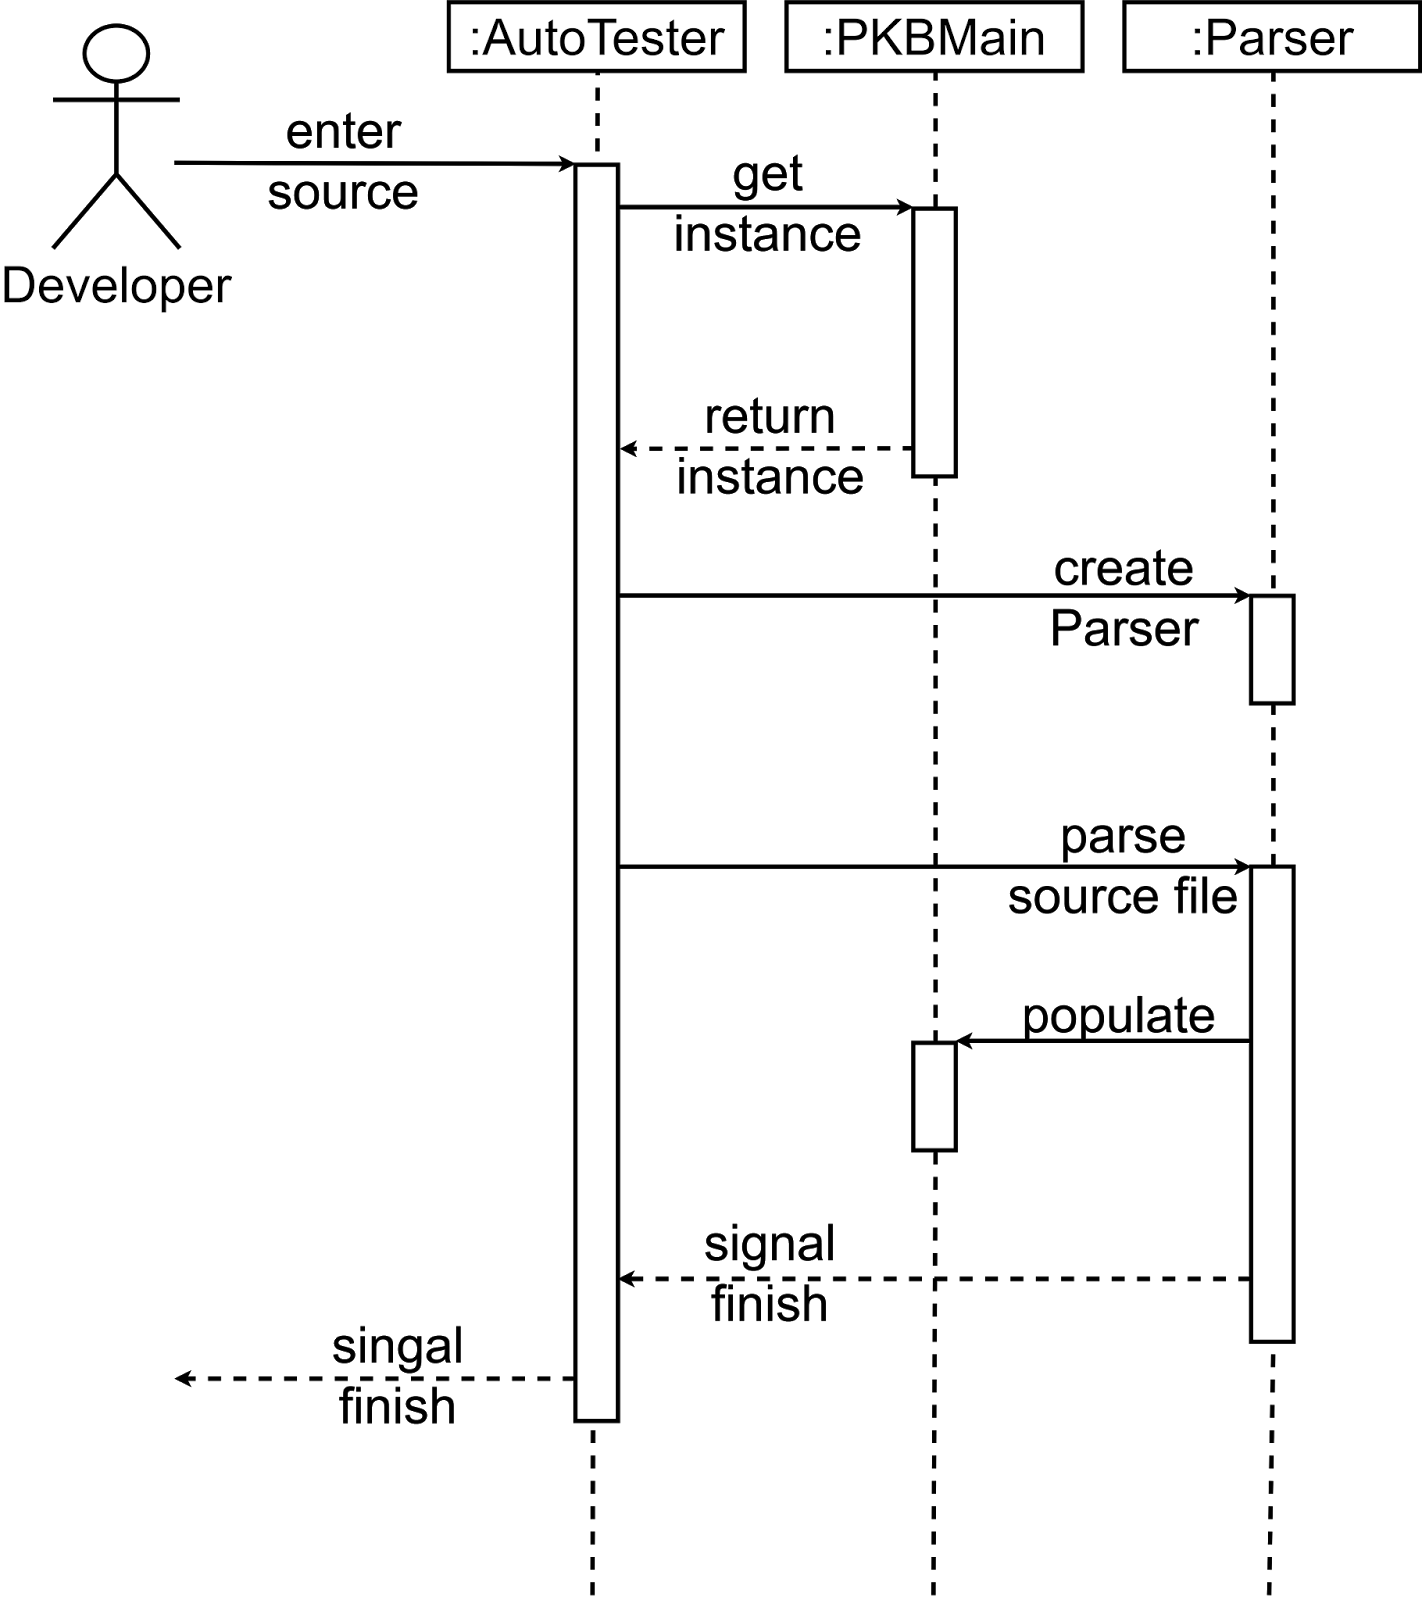
\includegraphics[width=0.8\textwidth]{SDTesting.png}
\end{figure}
\begin{tabular}{|L{5cm} | L{12cm}| }
\hline
\textbf{Test Purpose} &
The interaction between Parser and PKB is one-way, which involves the Parser populating PKB while parsing the SIMPLE source code.
 \\\hline
 \textbf{Required Test Input}
 &
SIMPLE source code \\\hline

\textbf{Expected Test Results}
 &
Stored information in PKB
 \\\hline

\end{tabular}

\begin{longtable}{|p{5cm} | p{12cm}| }
\hline
\textbf{Test Purpose} &
To test if PKB stores the relations in the parsed SIMPLE source code correctly.
\\\hline
\textbf{Required Test Input}
 &
 \texttt{
 \noindent TEST\_METHOD(TestNextRelation)
\newline \vspace{2mm} \hspace{4mm} //Set-up \newline
 \{ \hspace{2mm} list<int> actualResults; \newline \vspace{2mm}
 \hspace{4mm} list<int> expectedResults; \newline
  \hspace{4mm} Parser parser(pkbPtr); \newline
 \hspace{9mm}  Assert::IsTrue(parser.parse\newline(dummySimpleSourcePath));//set up previously \newline \vspace{2mm}
 \hspace{9mm} // Simple Next relations \newline
 \hspace{9mm} Assert::IsTrue(pkb.isNext(1, 2));\newline 
 \hspace{9mm} Assert::IsTrue(pkb.isNext(2, 3)); \newline \vspace{2mm}
 \hspace{9mm}  // Next relations when entering if-block\newline 
 \hspace{9mm}   Assert::IsTrue(pkb.isNext(4, 5));\newline 
  \hspace{9mm}   Assert::IsTrue(pkb.isNext(16, 17));\newline \vspace{2mm}
  \hspace{9mm}  // Next relations when entering else-block\newline 
 \hspace{9mm}   Assert::IsTrue(pkb.isNext(4, 6));\newline 
 \hspace{9mm}  Assert::IsTrue(pkb.isNext(16, 18)); \} }

 \\\hline
   \textbf{ Expected Test Results} &
true, true, true, true, true, true \\\hline
\end{longtable}
Helper methods are created to create dummy SIMPLE source codes and to destroy them at the end of the integration tests.
\newline
After parsing the dummy SIMPLE source codes and populating PKB, actual stored information is extracted using the API of PKB. This extracted data is then compared to expected ones.

\subsubsection{PQL - PKB SubSystem}
In this example, the components subjected to integration tests are QueryValidator and QueryTree.
\begin{figure}[H]
  \centering 
  \caption{Sequence diagram for PQL-PKB Interaction}
 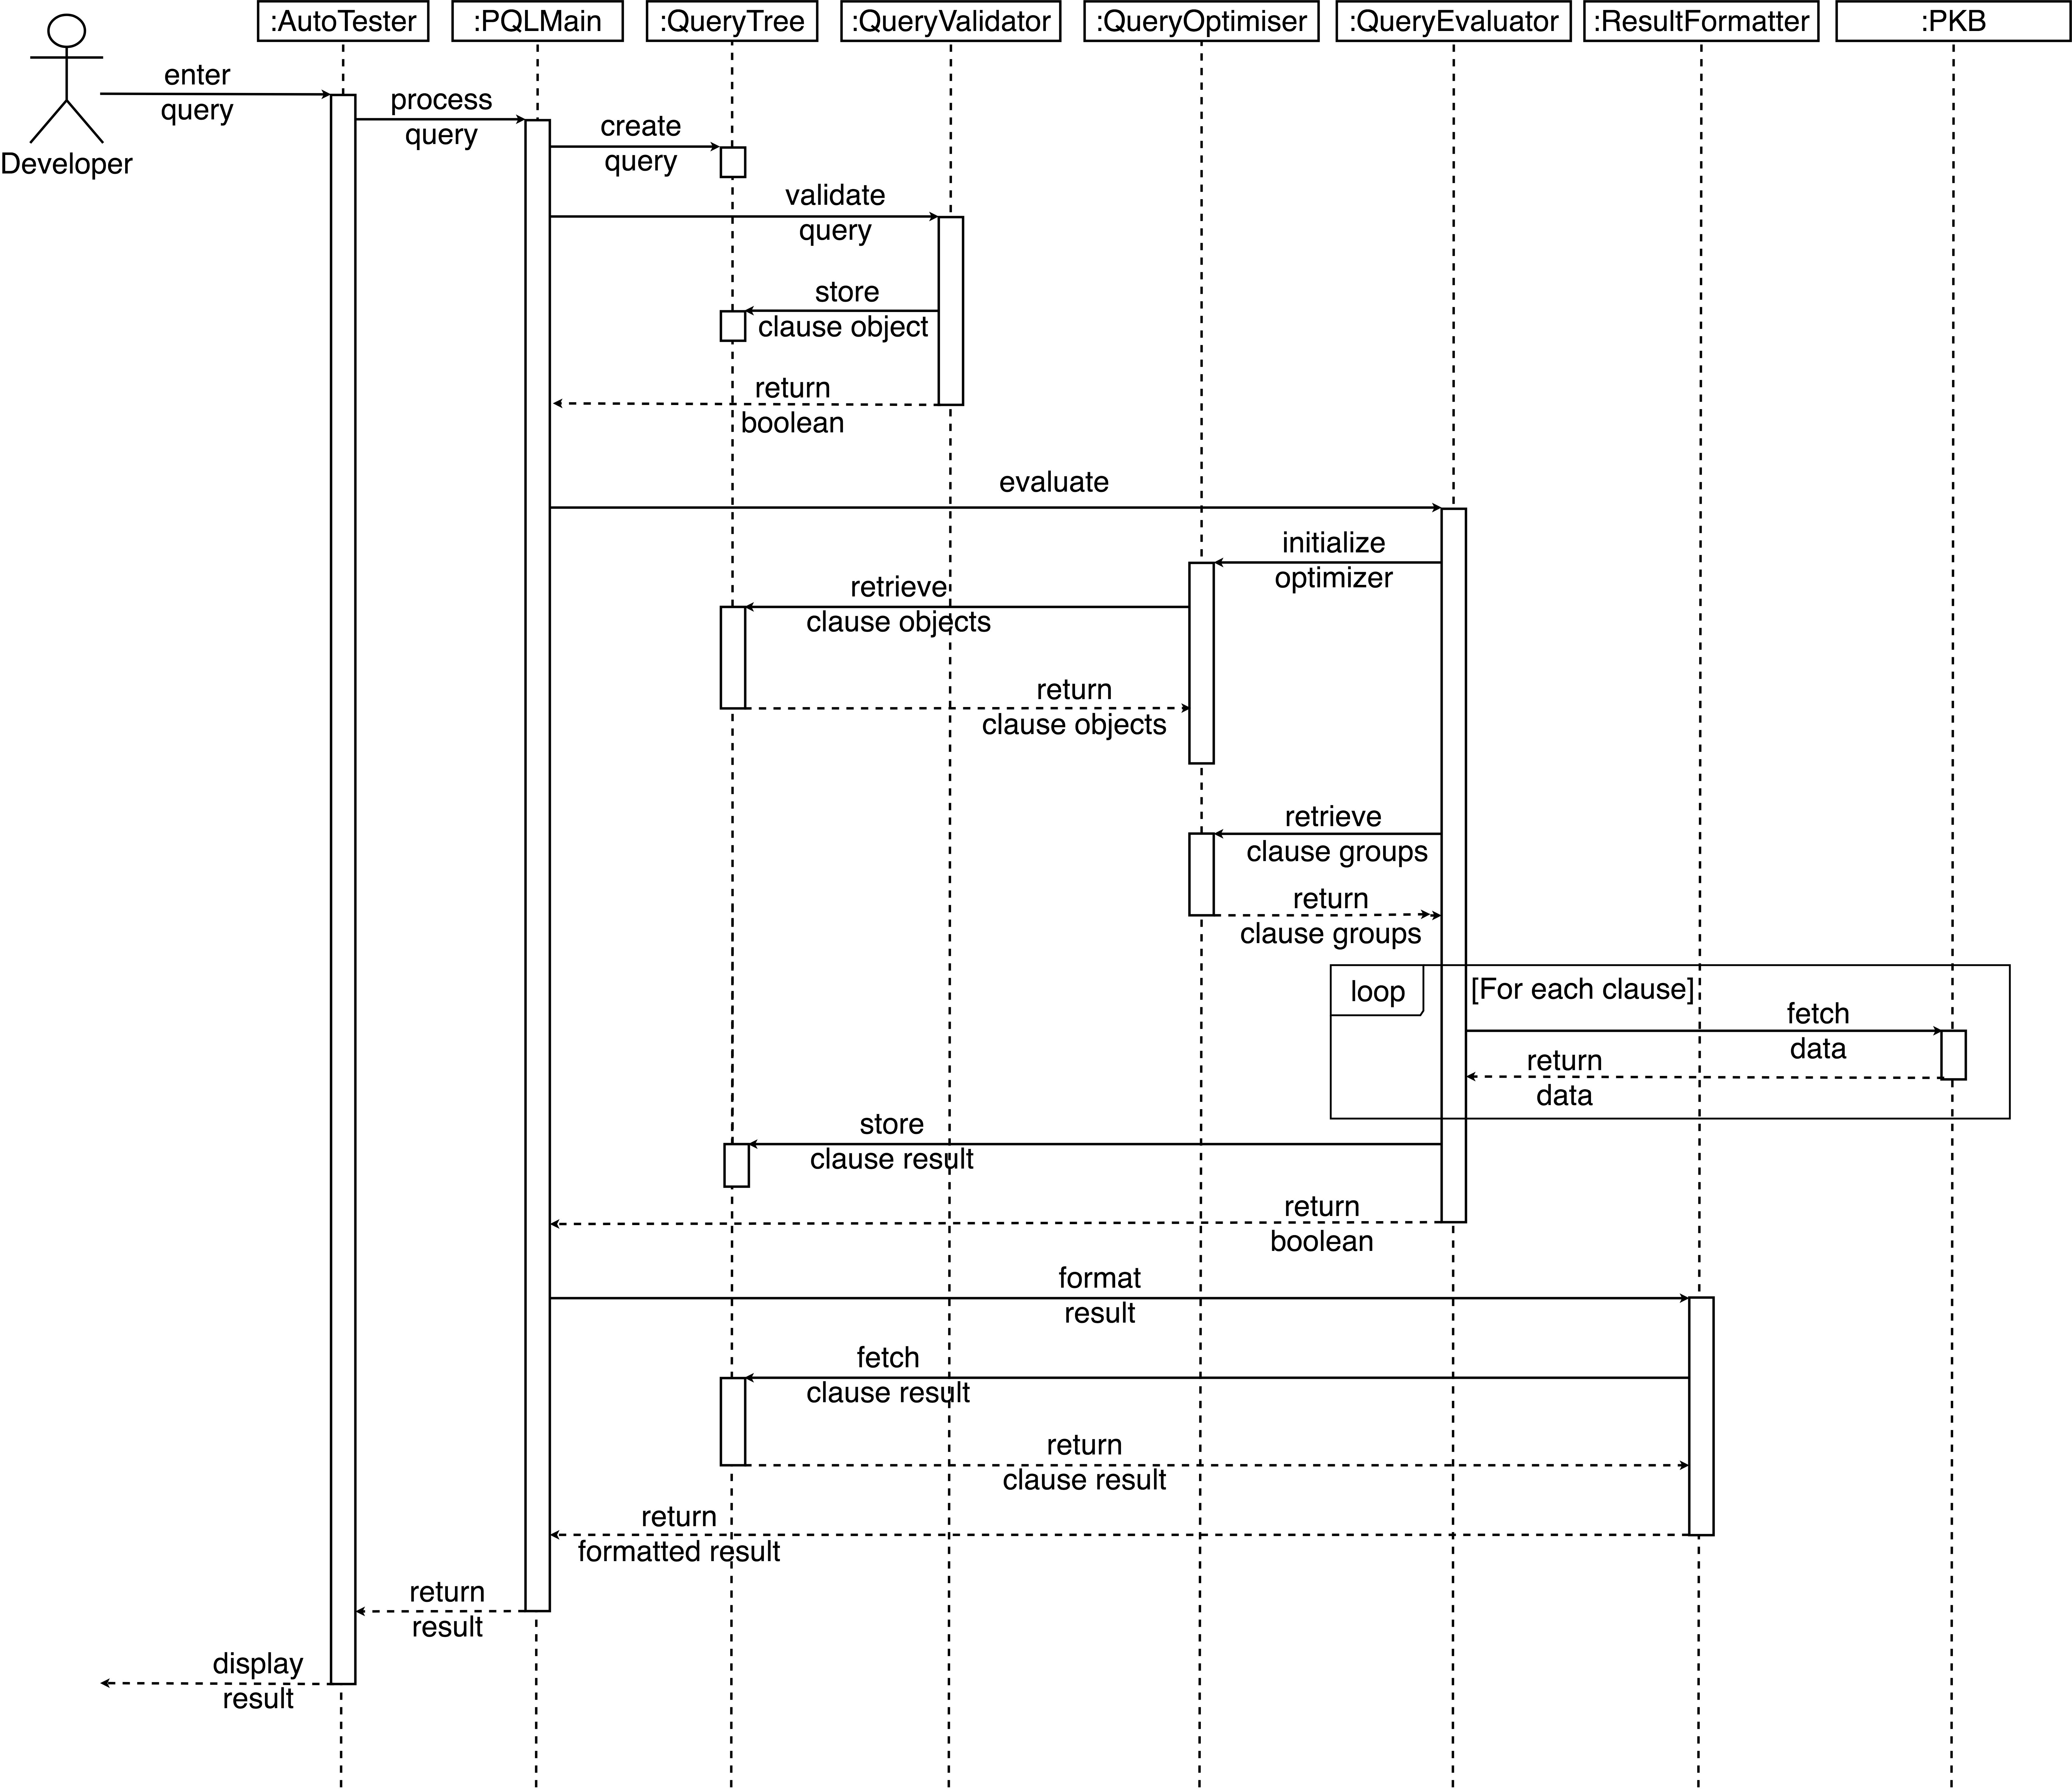
\includegraphics[width=1.0\textwidth]{PQL-PKB.png}
\end{figure}
\begin{longtable}{|p{5cm} | p{12cm}| }
\hline
\textbf{Test Purpose} &
To test if QueryValidator can validate complex query accurately and store the correct data into QueryTree. It specifically targets such that and pattern clauses of different combination.
\\\hline
\textbf{Required Test Input}
 &
\footnotesize
 \texttt{
 \noindent TEST\_METHOD(TestValidity\_Query\_\newline SelectSingleSynonym\_Stmt\_Parent\_Pattern\_Assign\newline \_And\_While\_SuchThat\_Follows\_And\_Modifies\newline \_Pattern\_Valid)
\newline \vspace{2mm}
 \{ \hspace{4mm} string query; \newline \vspace{2mm}
 \hspace{9mm} query.append("stmt s1, s2;"); \newline 
 \hspace{9mm} query.append("assign a1, a2;");\newline 
 \hspace{9mm} query.append("while w1, w2;");\newline 
 \hspace{9mm} query.append("variable v1, v2;");\newline 
  \hspace{9mm} query.append("Select s2 such that Parent(s1, s2) pattern a1(v2, \_) and w1(\"y\",\_) such that Follows(s2, s1) and Modifies(s1, \"x\") pattern w2 (v1, \_)"); \newline
    	\hspace{9mm}QueryTree qt; \newline
	\hspace{9mm}QueryValidator validator = QueryValidator(\&qt); \newline
	\hspace{9mm}Assert::IsTrue(validator.isValidQuery(query)); \newline
	\hspace{9mm}SelectClause expected = \newline UtilitySelection::makeSelectClause(SELECT\_SINGLE, STMT, "s2"); \newline
	\hspace{9mm}Assert::IsTrue(UtilitySelection::\newline isSameSelectClauseContent(expected, qt.getSelectClause())); \newline
	\hspace{9mm}vector<SuchThatClause> expectedListStc; \newline
	\hspace{9mm}vector<PatternClause> expectedListPc; \newline
	\hspace{9mm}expectedListStc.push\_back(UtilitySelection::\newline makeSuchThatClause(PARENT, STMT, "s1", STMT, "s2")); \newline
	\hspace{9mm}expectedListPc.push\_back(UtilitySelection::\newline makePatternClause(ASSSIGN\_PATTERN, "a1", VARIABLE, "v2", UNDERSCORE, "\_")); \newline
	\hspace{9mm}expectedListPc.push\_back(UtilitySelection::\newline makePatternClause(WHILE\_PATTERN, "w1", IDENT\_WITHQUOTES, "\"y\"", UNDERSCORE, "\_")); \newline
	\hspace{9mm}expectedListStc.push\_back(UtilitySelection::\newline makeSuchThatClause(FOLLOWS, STMT, "s2", STMT, "s1")); \newline
	\hspace{9mm}expectedListStc.push\_back(UtilitySelection::\newline makeSuchThatClause(MODIFIES, STMT, "s1", IDENT\_WITHQUOTES, "x")); \newline
	\hspace{9mm}expectedListPc.push\_back(UtilitySelection::\newline makePatternClause(WHILE\_PATTERN, "w2", VARIABLE, "v1", UNDERSCORE, "\_")); \newline
	\hspace{9mm}Assert::IsTrue(UtilitySelection::\newline AreSameSuchThatClausesContentAsInTree(expectedListStc, qt)); \newline
	\hspace{9mm}Assert::IsTrue(UtilitySelection::\newline areSamePatternClausesContentAsInTree(expectedListPc, qt));  \} }
 \\\hline
   \textbf{ Expected Test Results} &
true, true, true, true, true, true \\\hline
\end{longtable}


\normalsize
\subsection{System Tests}
System testing involves testing all components of the SPA together. This is carried out with the assistance of the AutoTester. Test cases are designed based on the considerations in Figure 26.
\begin{figure}[h]
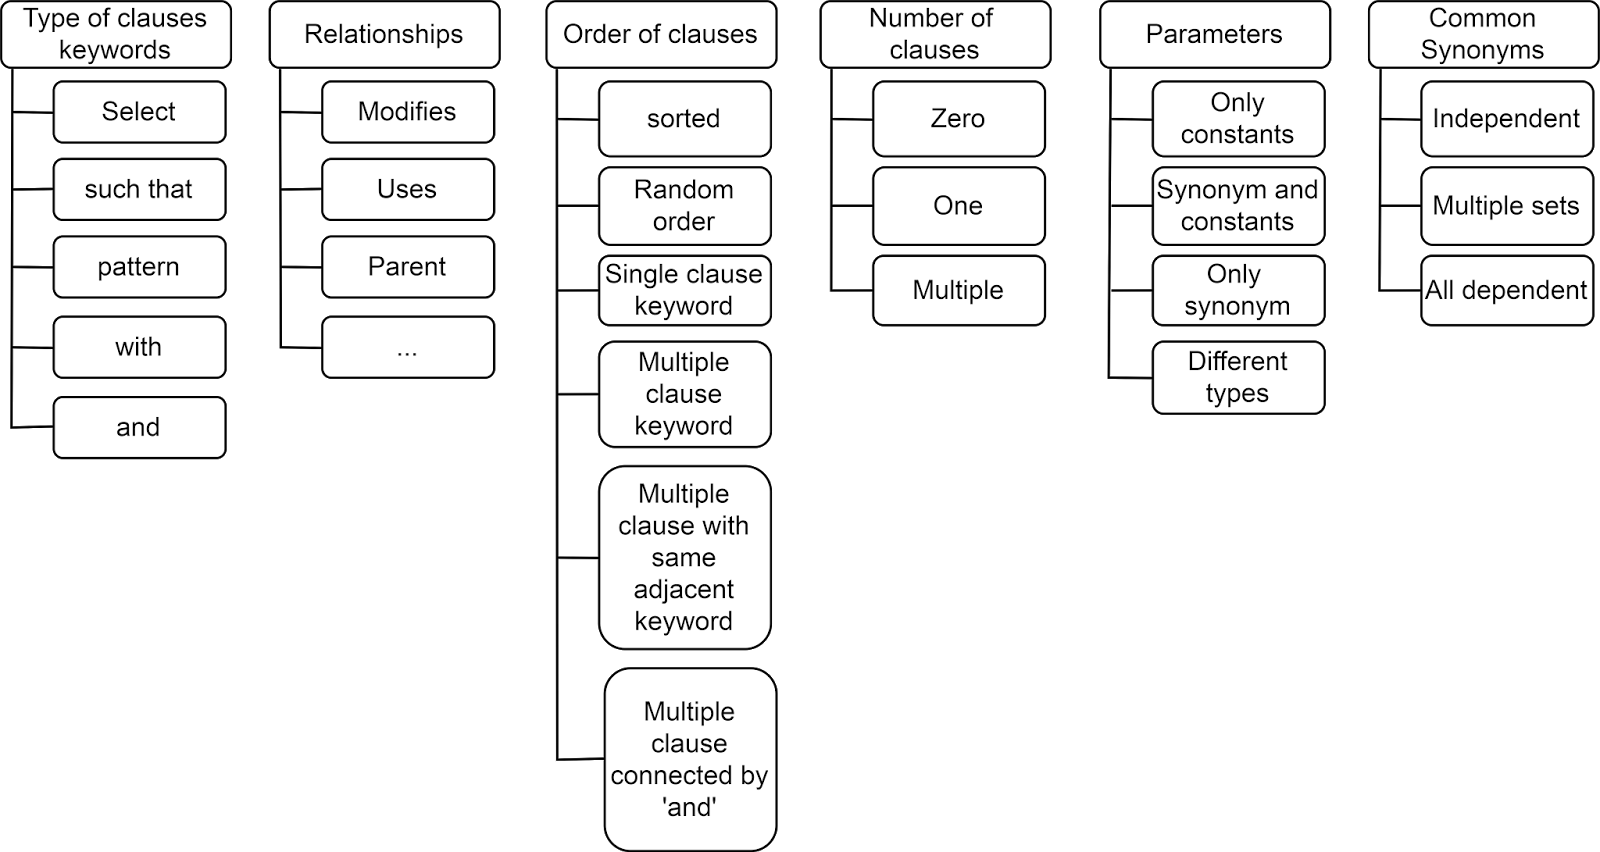
\includegraphics[width = 1.0\textwidth]{systemTesting.png}
\caption{System Testing}
\end{figure}
Test cases in system testing are controlled and run via a batch file.
System test queries are divided into 4 parts, namely:
\begin{enumerate}
\item Simple test queries
\item Complex test queries
\item Validation test queries
\item Stress test queries
\end{enumerate}

\textbf{Simple test queries} are defined as test cases which involve either no clause or only one such that/pattern/with queries. The purpose of these test is to test for each and every relationships and clauses. This can be used to debug PKB component or Query Evaluator component. For example:

\begin{verbatim}
stmt s;
Select s

stmt s;
Select s with s.stmt# = a.stmt#

assign a;
Select a pattern a(_,_”x”_)

stmt s; variable v;
Select s such that Uses(s,v)

while w1,w2;
Select w2 such that Parent*(w1,w2)
\end{verbatim}
They can also be in the form of one such that clause and one pattern/with clause, for example:
\begin{verbatim}
while w1,w2;
Select w2 such that Parent*(w1,w2) pattern w1(v,_)

stmt s; call c;
Select c such that Next*(a,c) with a.stmt# = 12

\end{verbatim}

\textbf{Complex test queries} are defined as test cases that involves multiple clauses, common synonym or all clauses, etc. The purpose of the complex queries not only test whether the queries are evaluated correctly, but also used to ensure optimiser is working properly so as to reduce Cartesian products.

For example:
\begin{verbatim}

while w1,w2; call c;
Select w2 such that Parent*(w1,w2) and Next(w1,c)

stmt s; assign a; variable v; procedure p;
Select <a,v> such that Uses(a,v) and Uses(s,v) with 
v.varName = p.procName

while w1,w2; assign a1,a2; if ifs; constant c;
Select <w1,w2,a1,a2> such that Affects*(a1,a2) such that Next(w1,ifs) 
with w1.stmt# = c.value such that Parent*(w2,a1) pattern a1(_,_"osaka"_)
\end{verbatim}

\textbf{Validation test queries} are defined as test cases that check the validity of the queries. The following queries are considered invalid due to error in syntax or declaration and thus returns ‘none’. The test is used in debugging the Query Validator component.

\begin{verbatim}
stmt s;
Select a

stmt s; variable v;
Select s such that Uses(s,v);

assign a;;;;
Select a

stmt s; stmt s;
Select s

stmt s;
Select s.varName
\end{verbatim}

The following system test queries check for whitespaces and they are considered valid and should return results accordingly.
\begin{verbatim}
stmt s;
Select     s      with     s.stmt     =     12

stmt s;
Select <   s   ,   s   >

stmt s;
       Select      s.stmt

\end{verbatim}

\textbf{Stress test queries} are queries that tests how many queries are computed on the fly (Next*, Affects and Affects*) and how many tuples our SPA can handle.The purpose of the stress queries is to evaluate the performance and effectiveness of the program under a heavy load. Example of such queries are shown:

\begin{verbatim}
stmt s1,s2,s3;
Select s1 such that Next*(s1,s2) and Next*(s2,s3)

stmt s1,s2,s3,s4;
Select s1 such that Next*(s1,s2) and Next*(s2,s3) and Next*(s3,s4)

stmt s1,s2,s3;
Select s1 such that Affects*(s1,s2) and Affects*(s2,s3)

stmt s1,s2,s3,s4;
Select s1 such that Affects*(s1,s2) and Affects*(s2,s3) 
and Affects*(s3,s4)

stmt s1,s2,s3;
Select <s1,s2> such that Affects*(s1,s2) and Affects*(s2,s3)

stmt s1,s2,s3;
Select <s1,s2,s3> such that Affects*(s1,s2) and Affects*(s2,s3)

\end{verbatim}

\subsubsection{Testing Methods}
The team has grouped similar test cases into the same folder. Each folder clearly describes its purpose, as shown in the table below. Do note that internally, we refer to our SPA as SPAXI.

\begin{figure}[H]
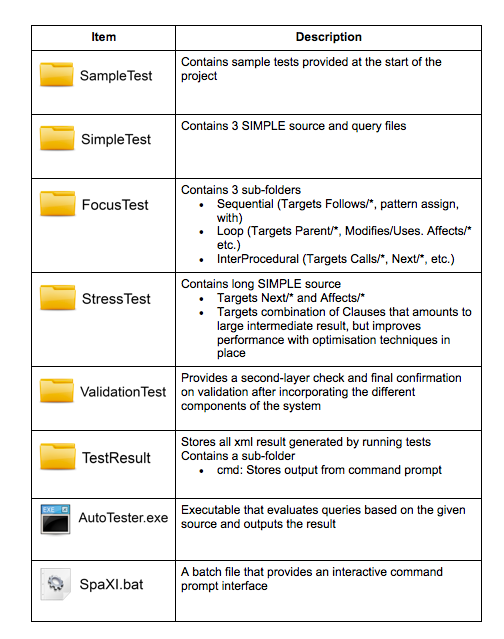
\includegraphics[width = 0.7\textwidth]{SystemtestingFolder.png}
\caption{Organization of Folders for System Tests}
\end{figure}
As there
are many query
 files to be written, the team came up with a way to automate testing. Firstly, for each of the folders above, an
  Excel spreadsheet i
  s created to hold all the queries, as shown in image Excel. In the Excel, there may contain more than one sheet. By using Excel, many repetitive work can 





























































be omitted. The autocomplete feature of Excel also helps in automatic numbering of index, as well as generating some of the queries. Secondly, a python script was written to assist the group in generating the q
uery text and converting them into text files shown in image query . Lastly, the team created a command prom

pt interface, called SpaXI, to facilitate the rest of testing. After which, results are stored in TestResult folder.

    \hspace{6mm}
    \begin{center}
      \begin{figure}[H]
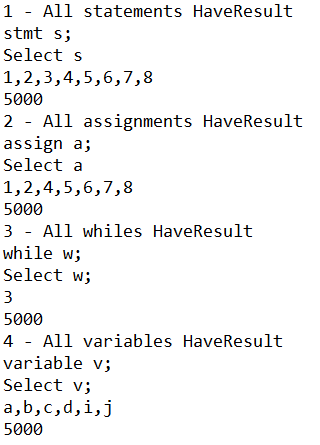
\includegraphics[width = 0.4\textwidth]{format.png}
\caption{Standard Query Format}
  \end{figure}
  \begin{figure}[H]
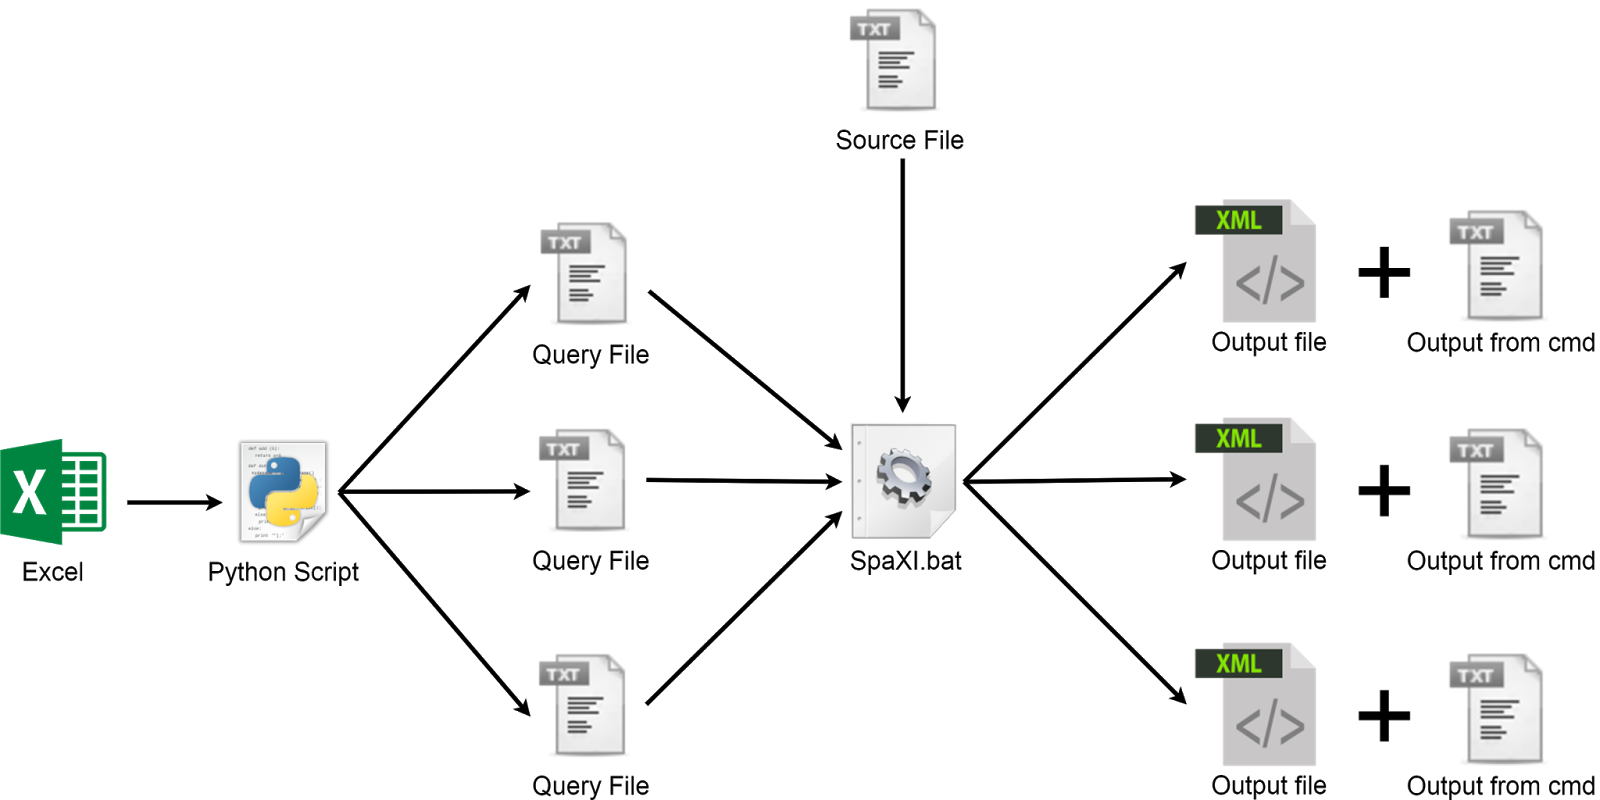
\includegraphics[width = 0.8\textwidth]{Flow.png}
\captionof{figure}{General flow of Automatic Testing}
  \end{figure}
    \end{center}
 \paragraph{Introducing SpaXI}
 SpaXI.bat, a batch file is created to provide an interactive command prompt interface for testing. The interface is shown below.
 \begin{figure}[H]
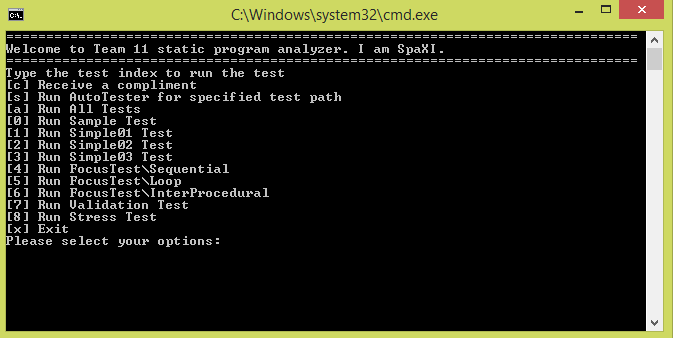
\includegraphics[width = 0.8\textwidth]{cmd.png}
\caption{SPAXI's Interface}
\end{figure}
\textbf{Command [c] :} To receive a compliment from SpaXi to brighten up your day \newline
\textbf{Command [s]:} To run an external source and query file provided by user \newline
\textbf{Command [a]:} To run all tests. At the end of the test, a summary text file will be generated, as shown in Figure 29. A tag called ‘BUG’ and/or ;TIMEOUT’ will be attached if the test fails or gets timed out. \newline
\textbf{Command [?]:} Enter the index of the test folder to run all the tests in that folder. (‘?’) represents an integer index. For example, if ‘3’ is entered as a command, SpaXi will run Simple03 Test.) \newline
\textbf{Command [x] :} Exit SpaXi \newline
 \begin{figure}[H]
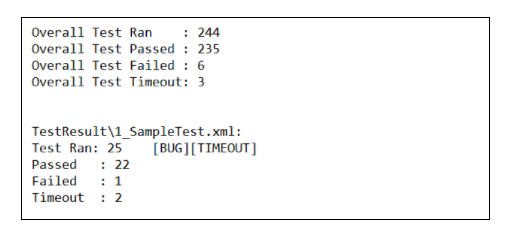
\includegraphics[width = 0.7\textwidth]{summary.png}
\caption{Summary of all tests run by SPAXI}
\end{figure}
\subsection{Sample Queries}
\begin{longtable}{|L{5cm} | L{12cm}| }
\hline
Test Purpose
 & To test if simple/complex queries produce the expected results that match SPA requirements.	\\ \hline
   Required Test Input &
1 - Select SingleSynonym Stmt Follows IntSynonym HaveResult \newline
stmt s; \newline
Select s such that Follows(1, s) \newline
2
\newline 5000 \newline
2 - Select SingleSynonym Stmt Parent IntSynonym BehindWhile HaveResult \newline
stmt s; \newline
Select s such that Parent(3, s) \newline
8
\newline 5000 \newline
3 - Select SingleSynonym Assign FollowsStar UnderscoreInt HaveResult \newline
assign a; \newline
Select a such that Follows*(a, 3) \newline
1,2,3,4,5,6,7,8
\newline 5000 \newline
4 - Select SingleSynonym Var Uses UnderscoreInt NoResult \newline
variable v; \newline
Select v such that Uses(v, "x") \newline
a, b, c
\newline 5000 \newline
5 - Select SingleSynonym  Modifies UnderscoreUnderscore Invalid \newline
variable v; \newline
Select v such that Modifies(\_, v) \newline
none
\newline 5000 \\ \hline
Required Test Input &
6 - Select SingleSynonym Call UnderscoreSynonym HaveResult \newline
call c; \newline
Select c.stmt\# such that Follows*(1, c) \newline
2,3
\newline 5000 \newline
7 - Select SingleSynonym Call Uses Synonym HaveResult \newline
call c; procedure p; \newline
Select c.procName such that Uses(p, "x") with c.procName = p.procName \newline
1
\newline 5000 \newline
8 - Select SingleSynonym Stmt FollowsStar SynonymInt NoResult \newline
stmt s; \newline
Select s such that Follows*(s, 1) \newline
none
\newline 5000 \newline
9 - Select SingleSynonym Stmt Parent SynonymInt BeforeWhile HaveResult \newline
stmt s; \newline
Select s such that Parent(s, 8) \newline
3
\newline 5000 \newline
10 - Select SingleSynonym Stmt Follows SynonymUnderscore HaveResult \newline
stmt s; \newline
Select s such that Follows(s, \_) \newline
1,2,3,4,5,6
\newline 5000
 \\\hline
\end{longtable}

\begin{tabular}{|L{5cm} | L{12cm}| }
\hline

Test Purpose
 & To test performance for complex queries, query optimiser, Affects and Affects*	 \\ \hline
   Required Test Input &
1 - Select SingleSynonym Stmt SuchThat Follows IntInt and Follows IntInt HaveResult
 \newline
stmt s; assign a; \newline
Select s such that Follows(1, s) and Affects(a, 10) with s.stmt\# =  a.stmt\#\newline
5, 6 \newline
5000 \newline

2 - 1 - 2 cmn syn + 1 cmn syn + 1 cmn syn
 \newline
assign a1,a2,a3,a4; stmt s; call cl; if ifs; while w; procedure p; variable v; \newline
Select ifs such that Next*(a1,a2) and Affects(a2,a3) with a3.stmt\#=s.stmt\# such that Parent(w,a4) pattern a4(\_,\_"tokyo"\_) such that Follows*(ifs,cl) and Uses(cl,v) with v.varName = p.procName
\newline
370,376,418 \newline
5000 \newline
3 - 1 - 3 Affects \newline
assign a1,a2,a3,a4; \newline
Select a3 such that Affects(a1, a2) and Affects(a2, a3) and Affects(a3, a4)\#\newline
3, 7, 17, 30, 32, 46, 47, 54, 56, 57, 59, 60, 61, 62, 63, 65, 67, 68, 83, 85, 86, 87, 89, 91, 92, 95, 96, 97, 99, 108, 113, 116, 117, 118, 121, 122, 124, 125, 127, 128, 131, 143, 144, 145, 147, 151, 153, 154, 156, 158 \newline
5000 \newline
3 -  2 - 4Affects
 \newline
assign a1,a2,a3,a4,a5; \newline
Select a4 such that Affects(a1, a2) and Affects(a2, a3) and Affects(a3, a4) and Affects(a4,a5)\newline
7, 32, 46, 47, 54, 56, 57, 59, 60, 62, 63, 65, 67, 68, 83, 85, 86, 87, 89, 91, 92, 95, 96, 97, 99, 113, 116, 117, 118, 121, 122, 124, 125, 127, 128, 131, 143, 144, 145, 153, 154, 156, 158 \newline
5000 \newline
4 - 4 - 6Affects
 \newline
assign a1,a2,a3,a4,a5,a6,a7; \newline
Select a6 such that Affects(a1, a2) and Affects(a2, a3) and Affects(a3, a4) and Affects(a4,a5) and Affects(a5, a6) and Affects(a6, a7)\newline
46, 47, 54, 56, 57, 59, 60, 62, 63, 65, 67, 68, 83, 85, 86, 87, 89, 91, 92, 95, 96, 97, 99, 113, 116, 117, 118, 121, 122, 124, 125, 127, 128, 131, 143, 144, 145, 153, 154, 156, 158 \newline
5000 \newline

5 - Select SingleSynonym Stmt SuchThat Follows IntInt SuchThat Follows IntInt HaveResult \newline
stmt s; assign a; var v; call c; \newline
Select a such that Parent*(1, a) and Follows(2, c) pattern a(v,\_"x"\_) with v.varName = c.procName \newline
2, 8 \newline
5000 
 \\\hline
\end{tabular}
\subsection{Testing Statistics}
\subsubsection{Unit Testing and Integration Testing}
We collectively wrote 983 unit tests and integration tests.
\subsubsection{System Testing}
\begin{enumerate}
\item Source Files (30-500 lines) : 9
\item Number of queries simple queries : 2009
\item Number of complex queries (including validation and stress tests) : 860

\end{enumerate}
\section{Discussion}
\subsection{Technical Difficulties}
For iteration 3, the t
echnical difficulties were minimal as the team was very familiar with Visual Studio 2015, C++ and Version Control.
\subsection{Project Management}
We discussed what could be improved following Iteration 2 and how we could further enhance our project management skills. We came up with mini-iterations for every week, and scheduled weekly meetings in 
order to ensure optimal working conditions and motivation for each team member to put their best effort in®. One team member was put in charge of scheduling and made sure to keep everyone on track. We also updat

























ed each other on any changes to be made to the schedule, but by and large we stuck to 
what we planned for this Ite






ration, and we can definitely say that our project management skills have improved. This way, we were also able to input consistent work.
\subsection{Workload and Time Management}
Two challenges we faced were trying to design an efficient algorithm to compute star relationships for Affects*, and how to system test effectively. However, with effective time management and divisions into mini-iterations, our team stuck to the deadline, and each member managed to complete these challenging tasks.

\begin{appendices}
\section{Documentation   of   Abstract   APIs} 
Given on the next page.
\end{appendices}
\end{document}